\documentclass[11pt,paper=letter]{scrartcl}

\usepackage[wide,boxthm]{cjquines}
\renewcommand{\v}[1]{\Var\sbr{#1}}

\begin{document}

\title{Machine learning}
\author{Carl Joshua Quines}
\date{July--August 2020}

\maketitle

\begin{abstract}
Notes for counselor seminars during PROMYS 2020. Standard disclaimer that I'm pretty clueless about machine learning, things are probably going to be badly explained, and even \textit{wrong}, etc. etc.
\end{abstract}

One of my perspectives of \textbf{machine learning} is that it's a toolbox to make predictions on data. Studying machine learning is like studying enumerative combinatorics. In a combinatorics class, maybe you'd learn about lots of different ways to count things, and solving a counting problem is a matter of choosing which one best fits the job. The same goes with machine learning.

Unlike, say, algebra or geometry, machine learning doesn't have a lot of central, unifying theories. It's just a general name for a collection of statistical tricks. This isn't a bad thing. It means that it only takes a little background knowledge to start reading about current research. (Though, the subfield of statistical learning theory is one important exception.)

I think I have two main goals in this seminar. First, I want to introduce the parts of machine learning that I think represent what's most interesting about the field, and showcase the larger issues of current research. And second, I want to talk about some of the state-of-the-art in machine learning.

I'll build up to this through speaking about three things. First is the \textbf{classification} problem and the approaches that are used to solve it, which I think is interesting and has some nice mathematical connections. This will lead us to \textbf{generalization} and some theoretical issues about data, which will touch on some statistical learning theory. Finally, we'll talk about \textbf{neural networks}, which have become so widely-used, that understanding them is often necessary, and sometimes even sufficient, if you want to read the latest research.

My main references are lecture notes from the Fall 2019 version of 6.036 Introduction to Machine Learning, \textit{The Elements of Statistical Learning}, and \textit{Foundations of Machine Learning}. If you look around, you can find Fall 2018 notes for 6.036, which are mostly similar to the Fall 2019 notes; I think they're good introductory notes. You can \href{https://web.stanford.edu/~hastie/ElemStatLearn//}{download Elements of Statistical Learning for free} on its website, which gives a broader discussion of many topics, though it's quite old. \textit{Foundations} is about statistical learning theory, and it's pretty probability-heavy, if you like that.

One last note. None of the figures here are intended to be \textit{really} accurate. All the decision boundaries and regressions are eyeballed, and are intended to just give an idea of what it should actually look like. But that's fine, it's like how geometry figures don't have to be to scale, right?

\clearpage

\section{Classification (July 19)}

\textit{Prerequisites:} Know what a linear regression is, but not necessarily how to do it, dealing with matrices, vectors, conditional probability, Bayes's theorem. Nice, but not necessary: matrix differentiation, multivariate Gaussians.

\subsubsection*{A first example}

Here's a machine learning problem. We have some points in the plane. Some are circles and some are crosses. Here's a picture:

\begin{center}
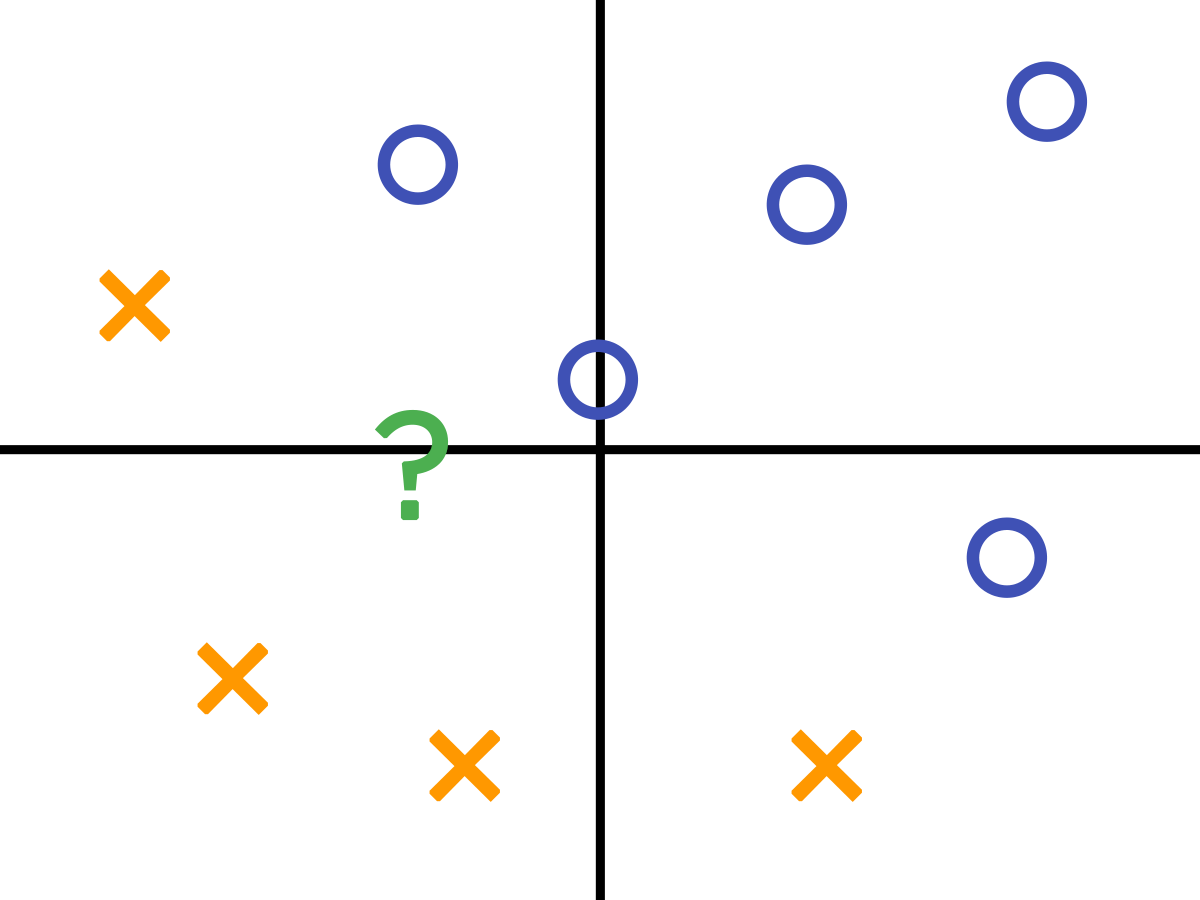
\includegraphics[height=2in]{1.png}
\end{center}

This is your training data. Now consider the question mark. Do you think it's more likely to be a circle or a cross?

Here are two ways to solve this problem. First is \textbf{linear regression}. We're going to take our plane and add another dimension, the height, based on whether it's a circle or a cross. We'll make the height of a point $1$ if it's a circle, and $-1$ if it's a cross. Plotting in space, rather than the plane, we get this:

\begin{center}
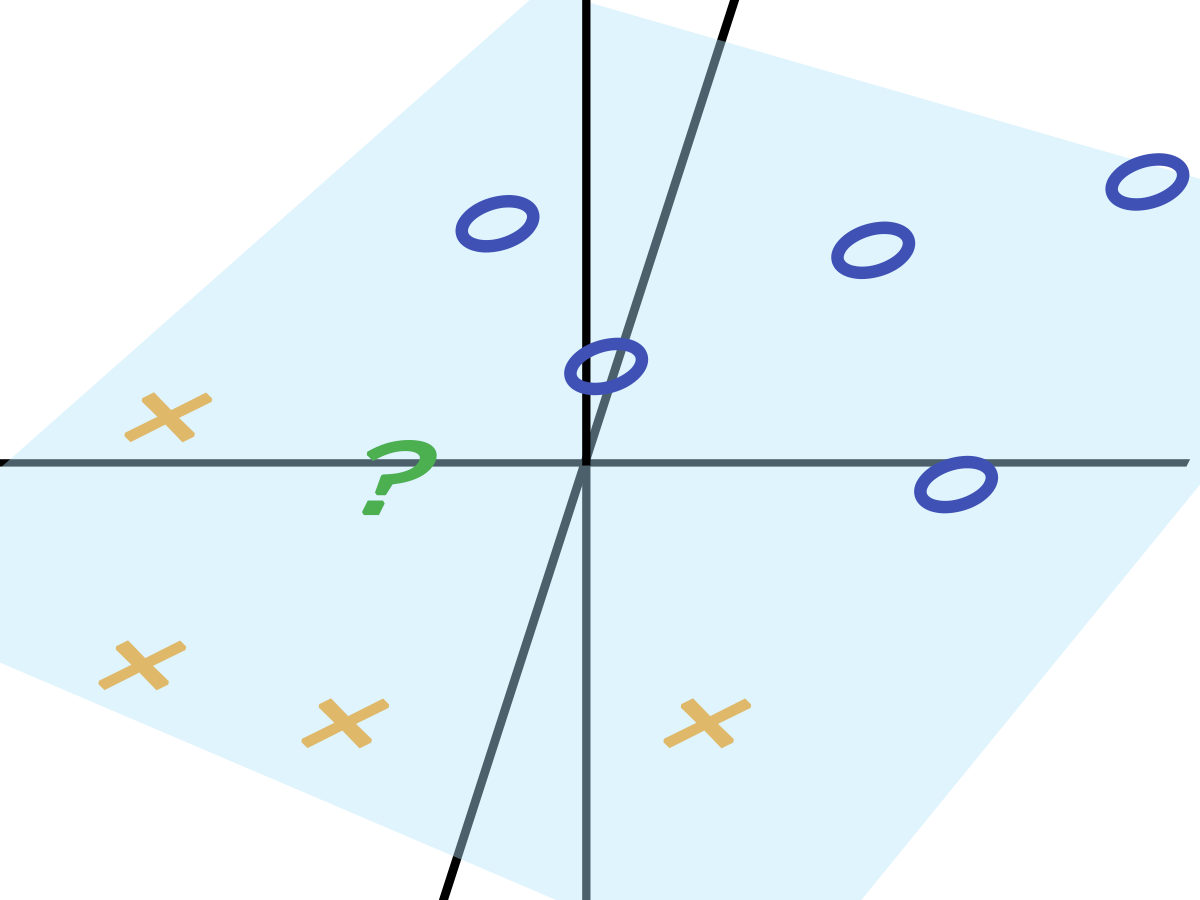
\includegraphics[height=2in]{2.png}
\end{center}

Now apply linear regression on the new training data. This will give us a plane that tries to match the location of these points.

We can think of a plane as taking $x$- and $y$-coordinates, and returning a height, or a $z$-coordinate. This plane will now be our model. We'll say that a point is a circle if its height is positive, and a cross if its height is negative. According to this model, the point is a cross.

Second is \textbf{nearest neighbors}. This is arguably a simpler way. We take the point nearest to the question mark among the training data, and if it's a circle we say it's a circle, and if it's a cross we say it's a cross. According to this model, the point is a circle.

Of course, rather than plugging into the hyperplane formula, or looking at the nearest neighbors every time, we can look at the \textbf{decision boundaries}. For the hyperplane, the decision boundary is the line where $z = 0$. Everything ``above'' that line is a circle, and everything ``below'' that line is a cross. For nearest-neighbors, the boundaries are polygons that are drawn around the data. Everything that falls within a circle boundary, we say is a circle; everything that falls within a cross boundary, we say is a cross:

\begin{center}
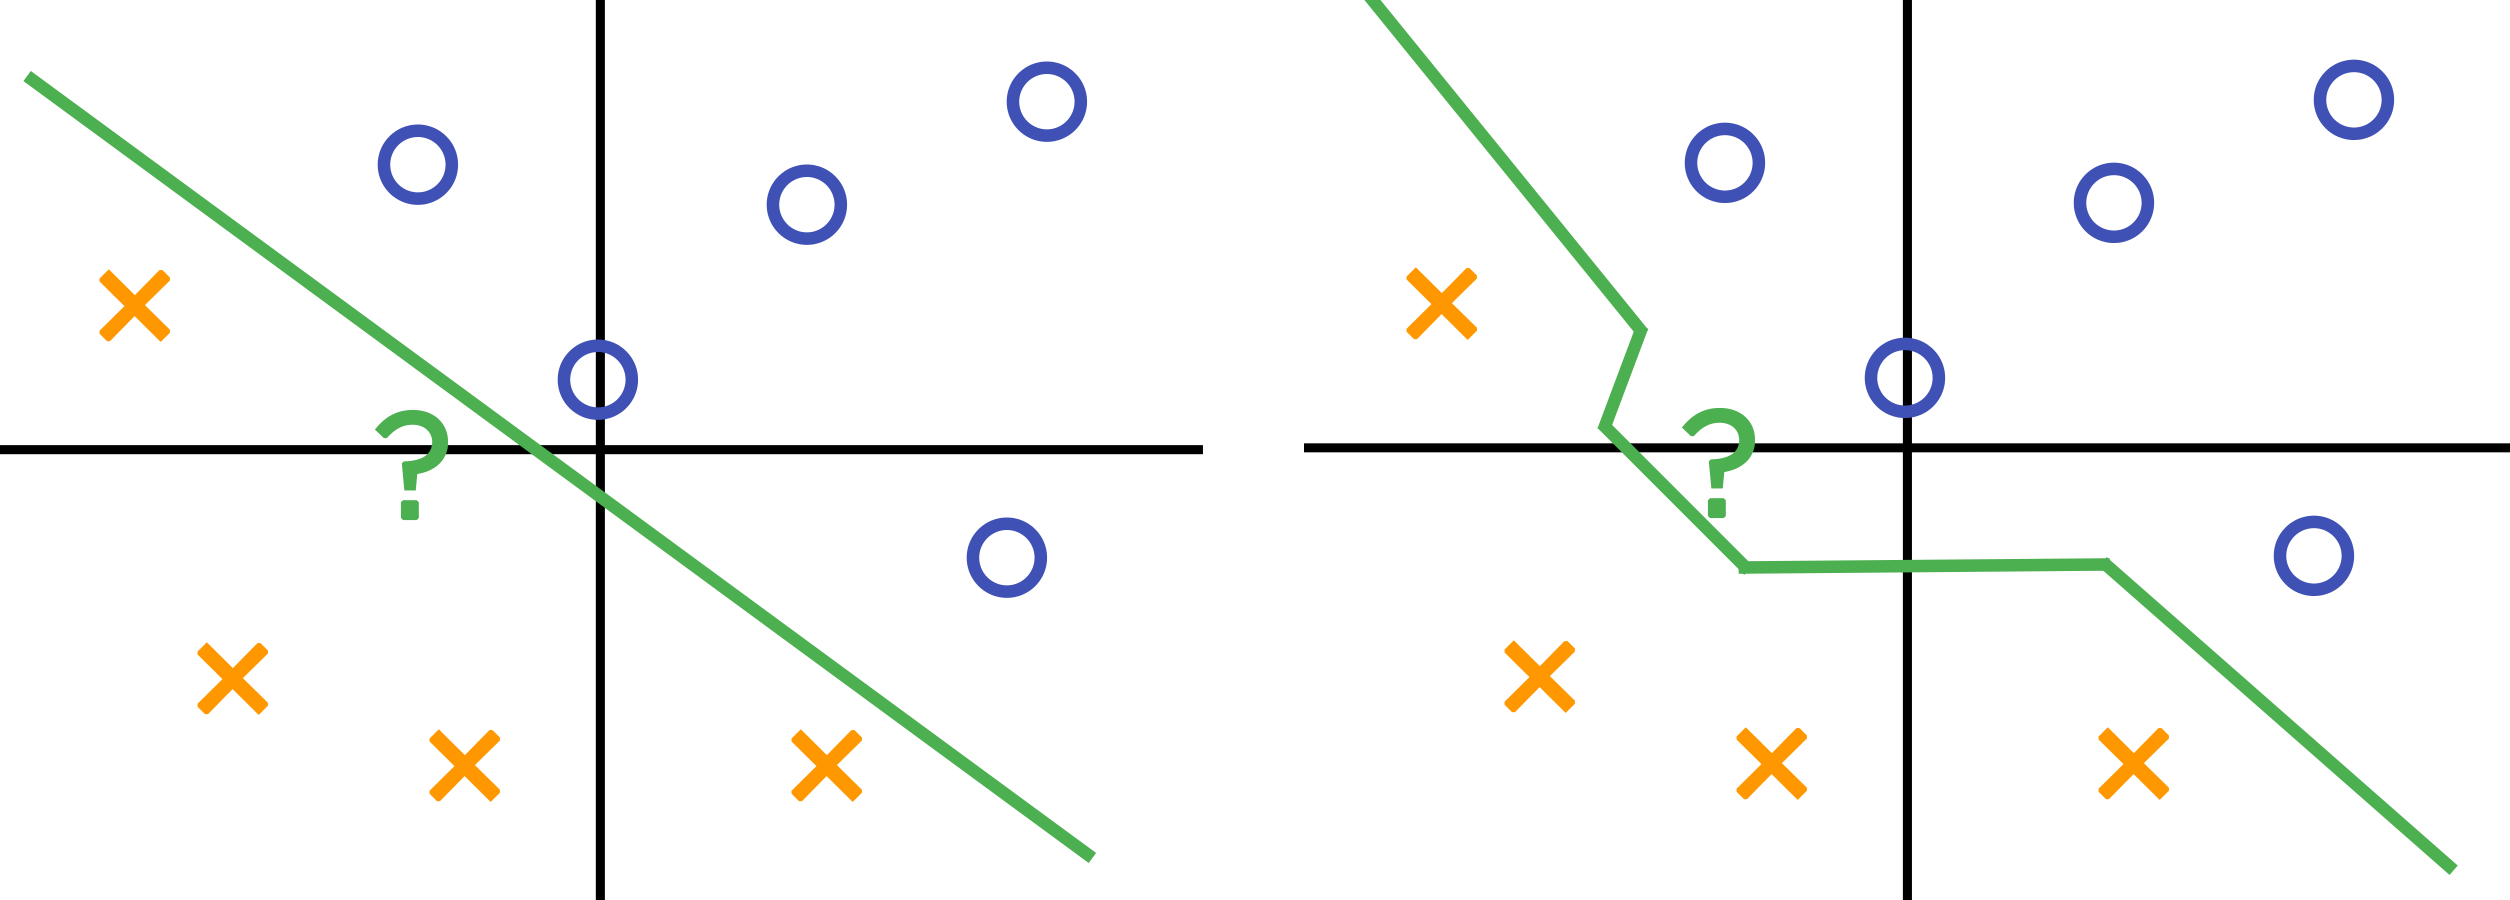
\includegraphics[height=1.8in]{3.png}
\end{center}

How do linear regression and nearest neighbors stack up with different kinds of data? Here's another example of circles and crosses in the plane, along with the decision boundaries of linear regression and nearest neighbors:

\begin{center}
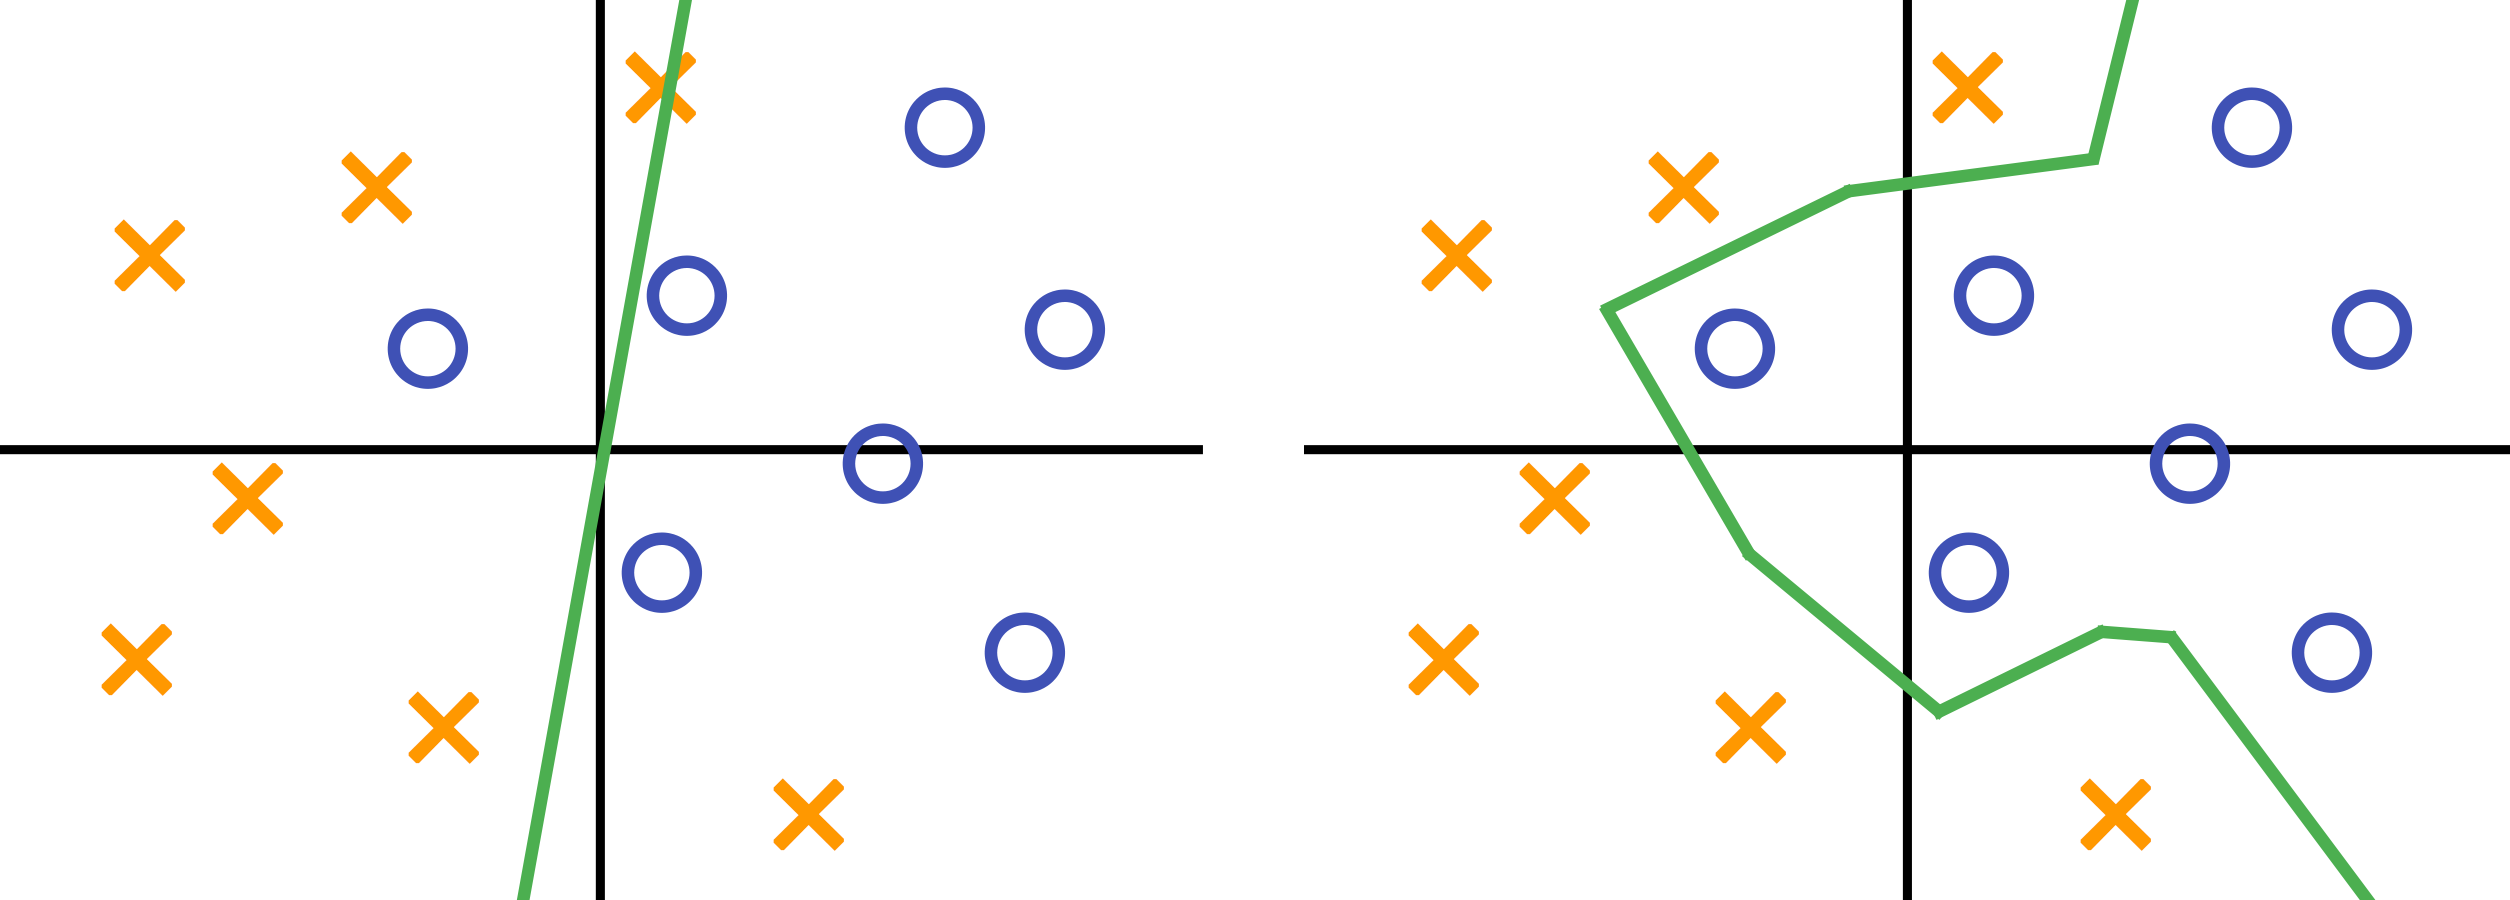
\includegraphics[height=1.8in]{4.png}
\end{center}

Which one do you think is more likely to be ``true'', whatever that means? What about in this scenario:

\begin{center}
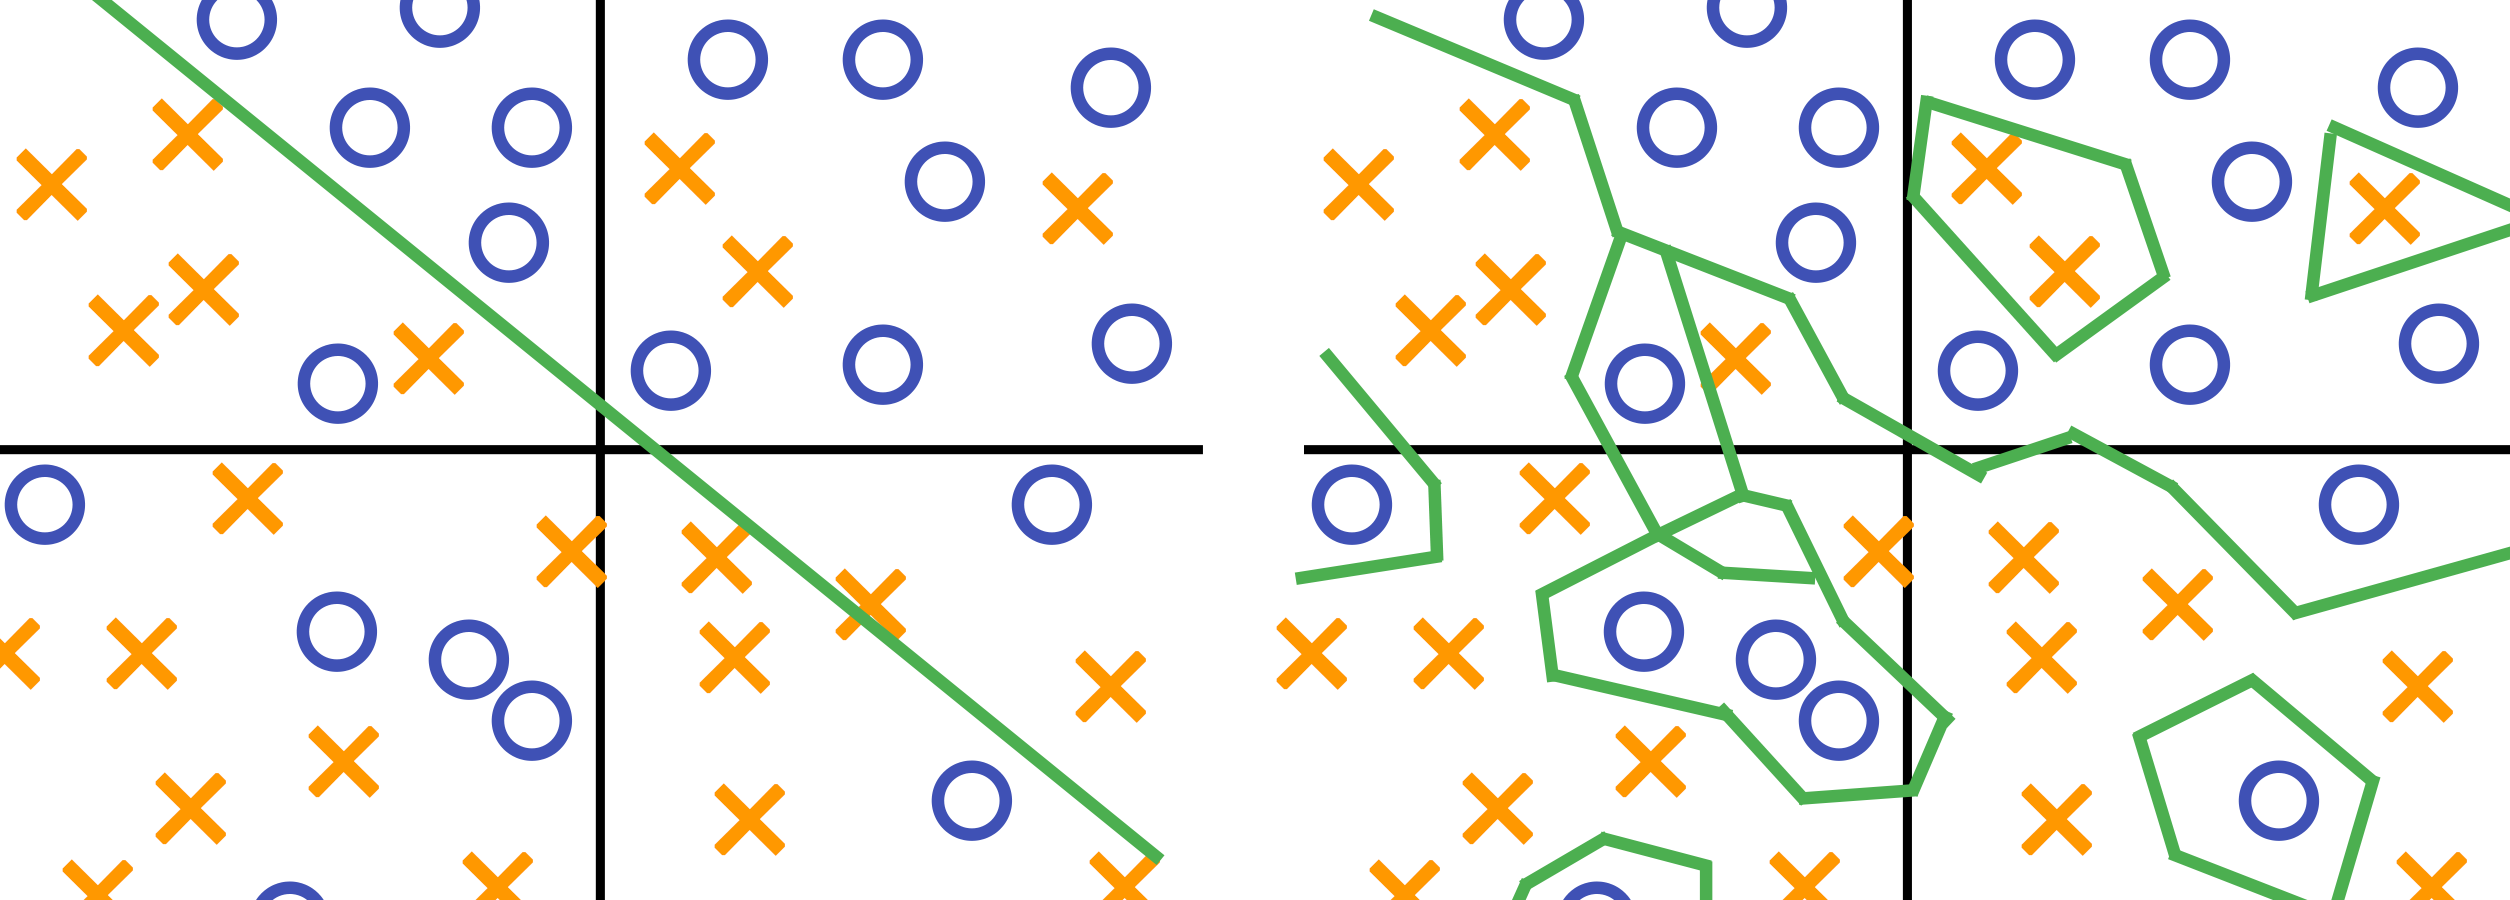
\includegraphics[height=1.8in]{5.png}
\end{center}

Maybe nearest neighbors is too ``sensitive''. Instead of taking just the nearest neighbor, why don't we take the $3$ nearest neighbors, and then do a majority vote. If circle is the most common among the $3$ nearest neighbors, say it's a circle. If it's cross, say it's a cross.

In fact, we can generalize beyond $3$. Let's call the general algorithm $k$-nearest neighbors. Here's what the decision boundaries looks like for different $k$. In reading order, this is $k = 1$, then $k = 3$, then $k = 9$, and finally, $k = 50$. In the last one, the entire plane is classified as a cross, as there are more crosses than circles.

\begin{center}
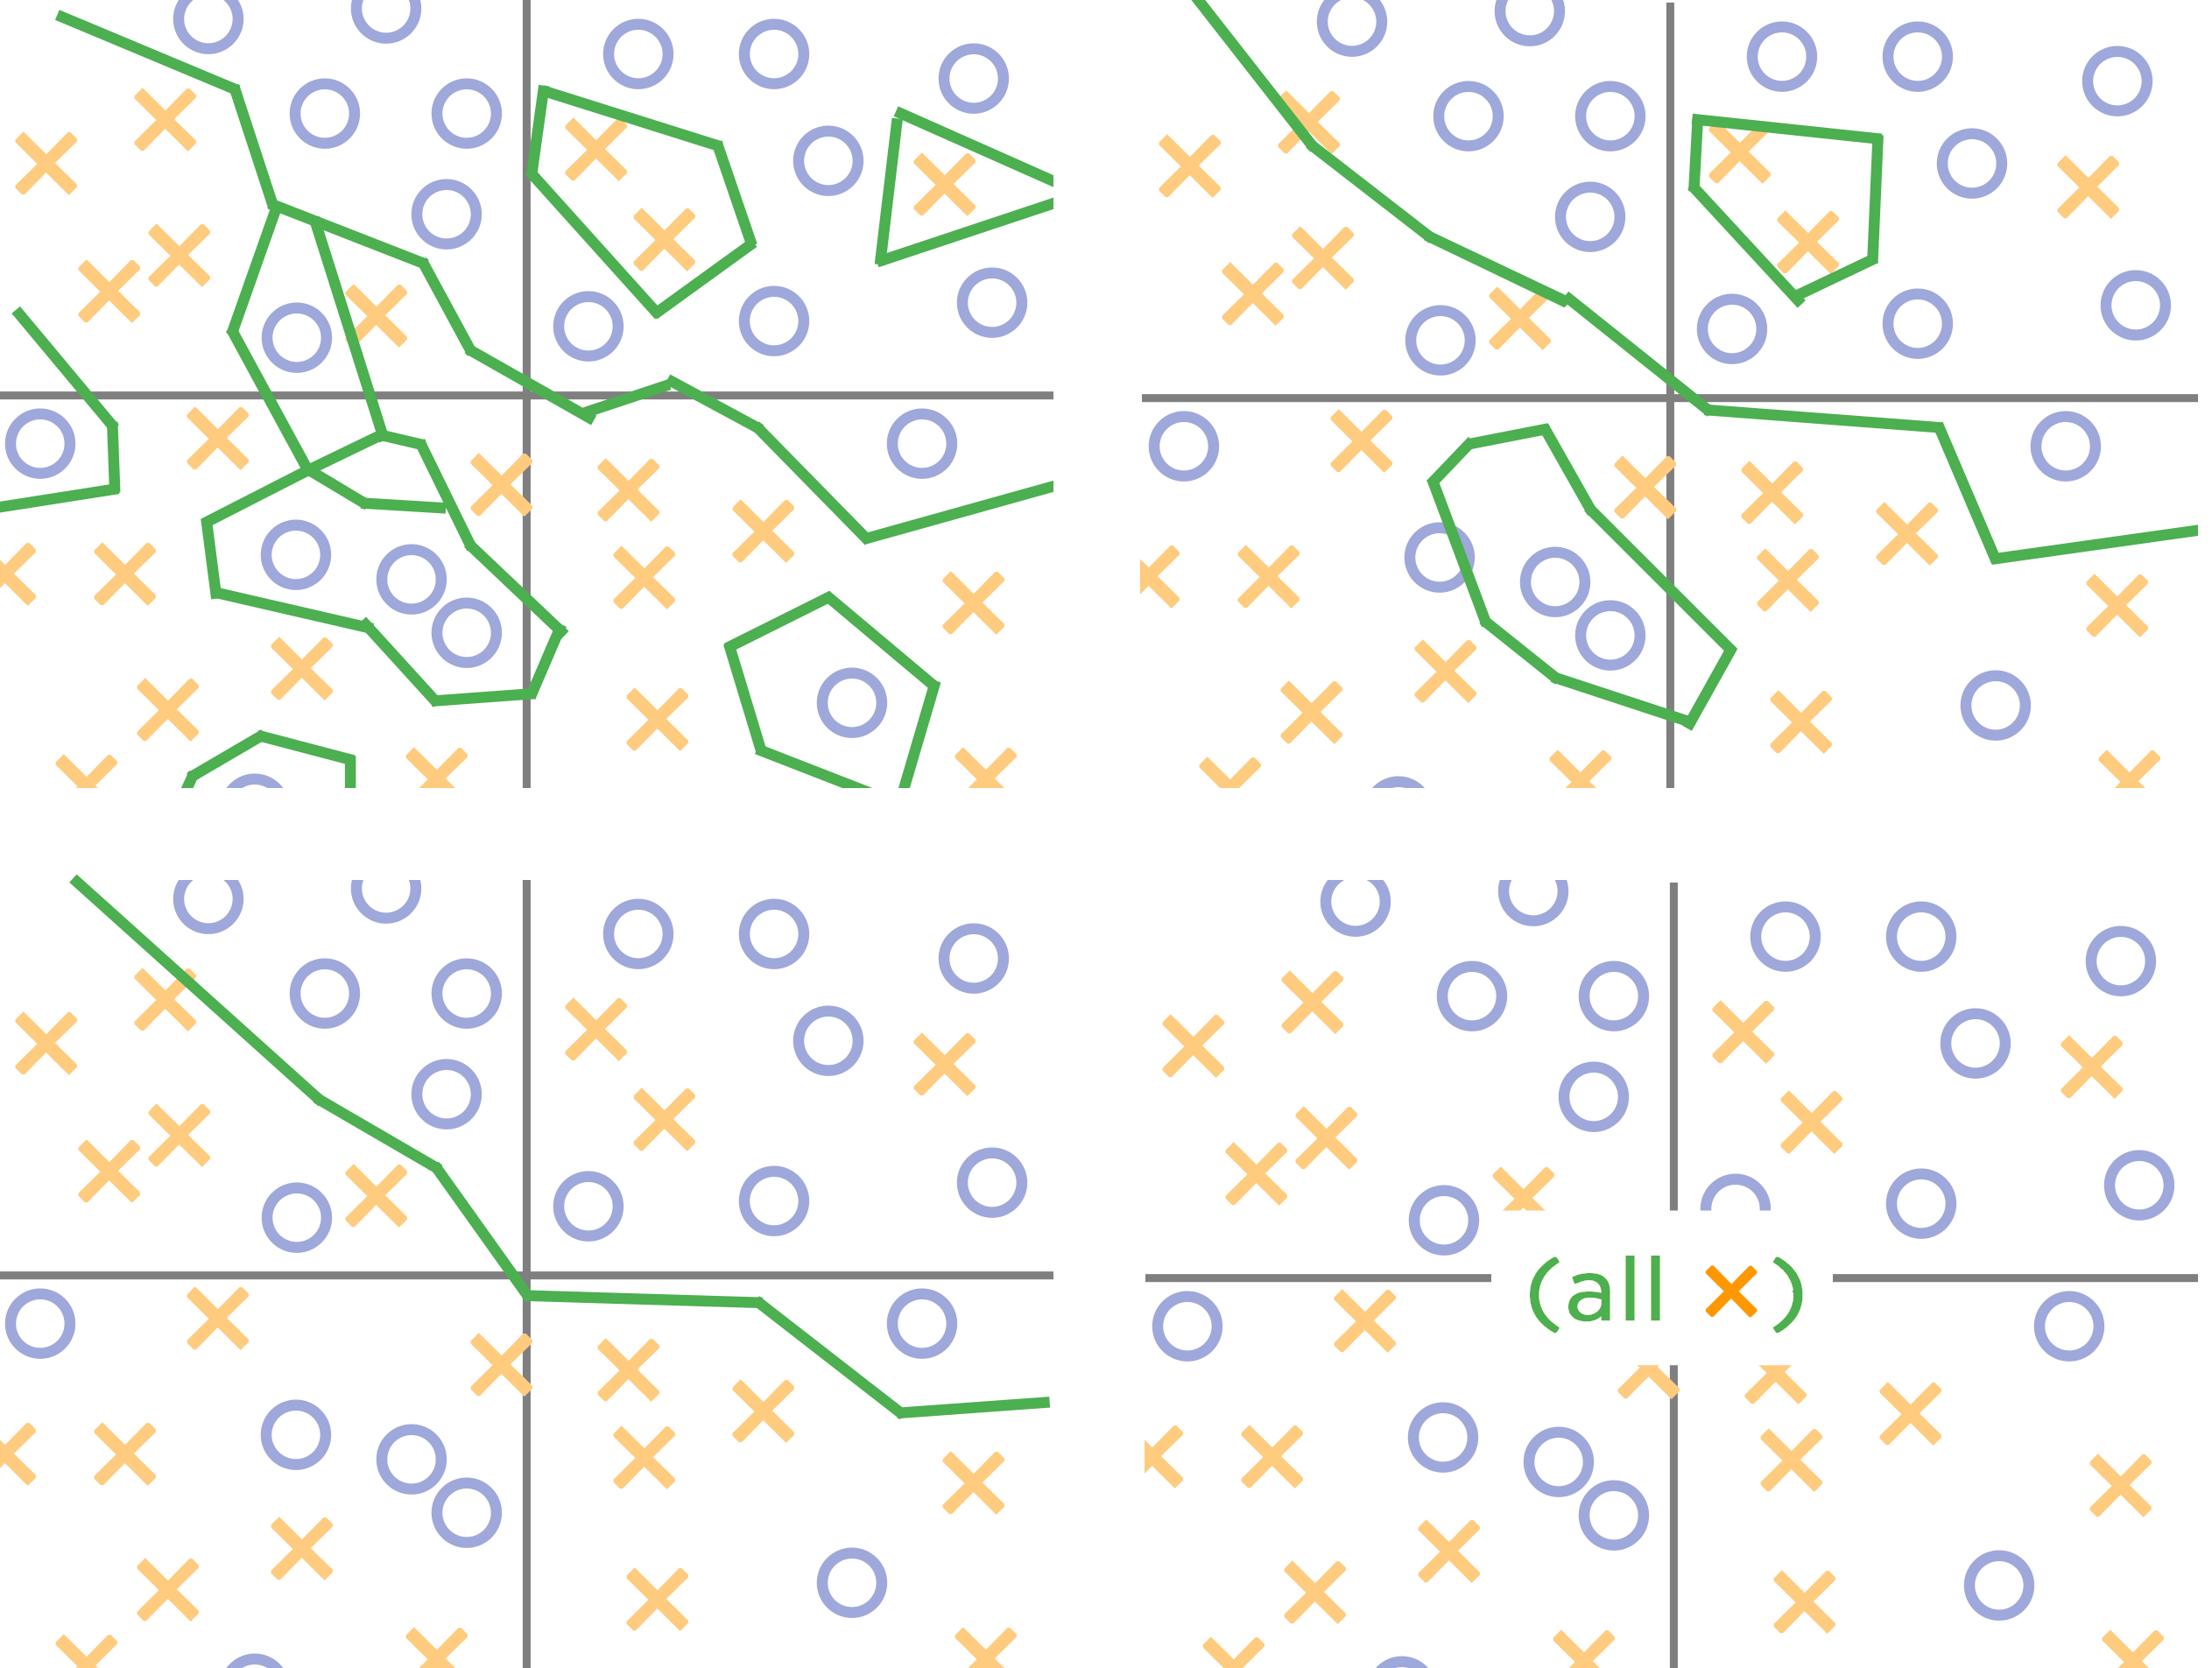
\includegraphics[height=4in]{6.png}
\end{center}

Which of these is the ``best''? How does this compare with linear regression? Are there better ways to find classifiers? How do we choose $k$? How do we choose between models, anyway?

\subsubsection*{Definitions}

We'll return to some of these questions shortly, but now that we have some experience, we're ready to define some terms.

Machine learning is about \textbf{learning algorithms}, or ``tools'' in our toolbox analogy. Depending on the kind of problem, we'll throw a different learning algorithm at it. A learning algorithm takes in \textbf{data} and produces a \textbf{model} or \textbf{hypothesis}. It's the model that we use to make predictions or analyze data.

Take note of the types. Generally, data has type (input, output), a model has type input $\to$ output, and a learning algorithm has type data $\to$ model. In the first example earlier, the data is the points and their labels, the model is plugging it into the plane equation and determining whether it's above or below $z = 0$, and the learning algorithm is linear regression that produces this plane in the first place.

The problem we've been looking at so far is called \textbf{classification}: classify these inputs into a discrete set of outputs. The model in this case is called a \textbf{classifier}. There are other kinds of problems too, like regression, ranking, clustering, and so on. For this and the next seminar we'll focus on classification.

Sometimes the learning algorithm doesn't just take in the data, but some other inputs. For example, $k$-nearest neighbors takes the examples, but it also takes the input $k$, for how many neighbors to look at. We call $k$ a \textbf{hyperparameter}: it's something that goes into the learning algorithm that isn't the data itself.

The data is usually called \textbf{examples}. The examples are usually split up into \textbf{training data}, \textbf{validation data}, and \textbf{test data}. Training data is what's fed into the learning algorithm. Validation data is used to pick the hyperparameters. Test data is used to measure how good the produced model is, using something called a \textbf{loss function}; an example of a loss function might be squared loss. (It is one thing to test a model, it is another thing to test a learning algorithm!)

In our previous example, the test data was conveniently given as points in the plane, but this is rarely the case in real life. Data comes as words, pictures, music. Our learning algorithms assume all input and output are numbers, or vectors. So we convert this data into \textbf{features}. If we wanted to write a machine to distinguish plants from animals, it could taken in features like height, weight, color, and so on. Doing this is the task of \textbf{feature extraction}, or feature representation.

Finally, the outputs in the data are called \textbf{labels}. So we can think of data as pairs of features and labels. That was a lot of words. Here's a diagram:

\begin{center}
  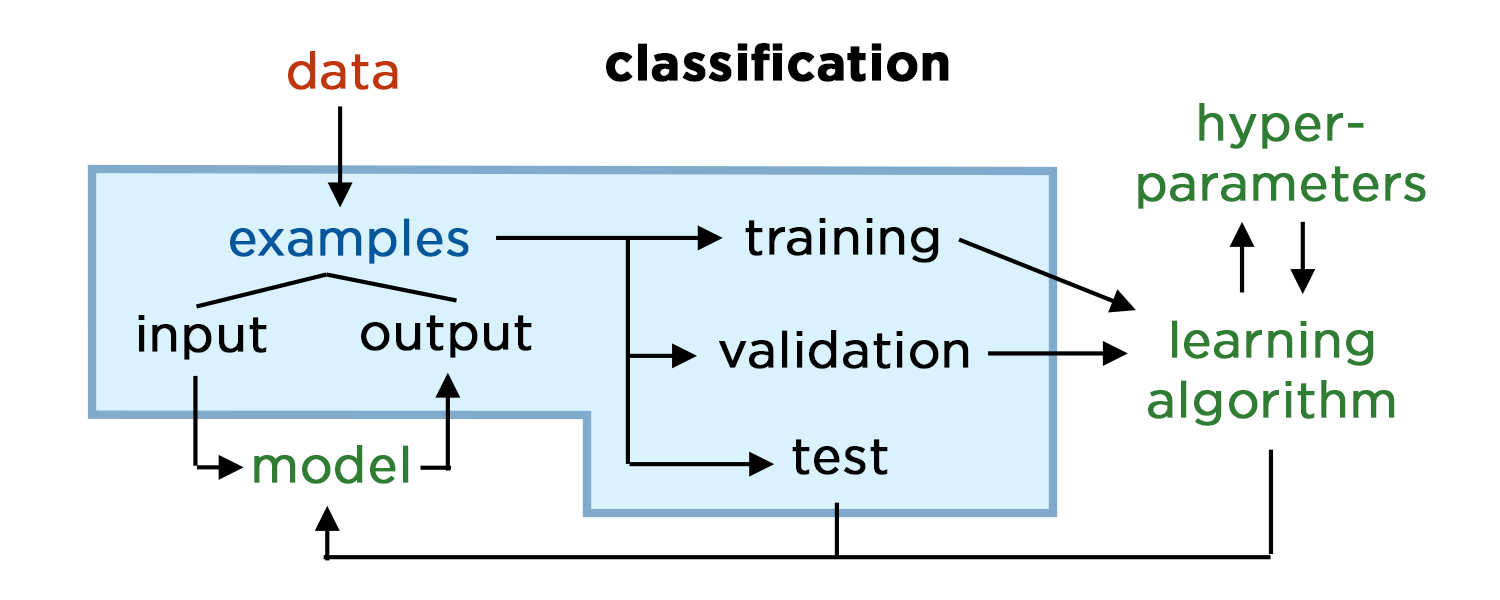
\includegraphics[height=1.8in]{7.png}
\end{center}

\subsubsection*{Linear regression}

Let's go back to our previous questions. For the rest of the hour, we'll tackle the classification problem using \textbf{linear classifiers}, or classifiers with linear decision boundaries. (These sound pretty specific, but we'll show later how they easily generalize.)

Let's recall some facts about linear regressions. In the simple case, we'll have a $d$-dimensional input vector $x = (x_1, x_2, \ldots, x_d)^T$, which corresponds to some scalar output $y$. The hyperplane that will fit the data will be of the form \[
  f(x) = \beta^Tx + \beta_0,
\]
for some $d$-dimensional vector $\beta$, and some scalar $\beta_0$. We can simplify this by augmenting $x$ to $x' := (1, x_1, \ldots, x_d)^T$, and augmenting $\beta$ to $\beta' := (\beta_0, \beta_1, \ldots, \beta_d)^T$. Our fitting hyperplane is now $f(x') = \beta'^Tx'$, which passes through the origin. Geometrically, this is projectivization:

\begin{center}
  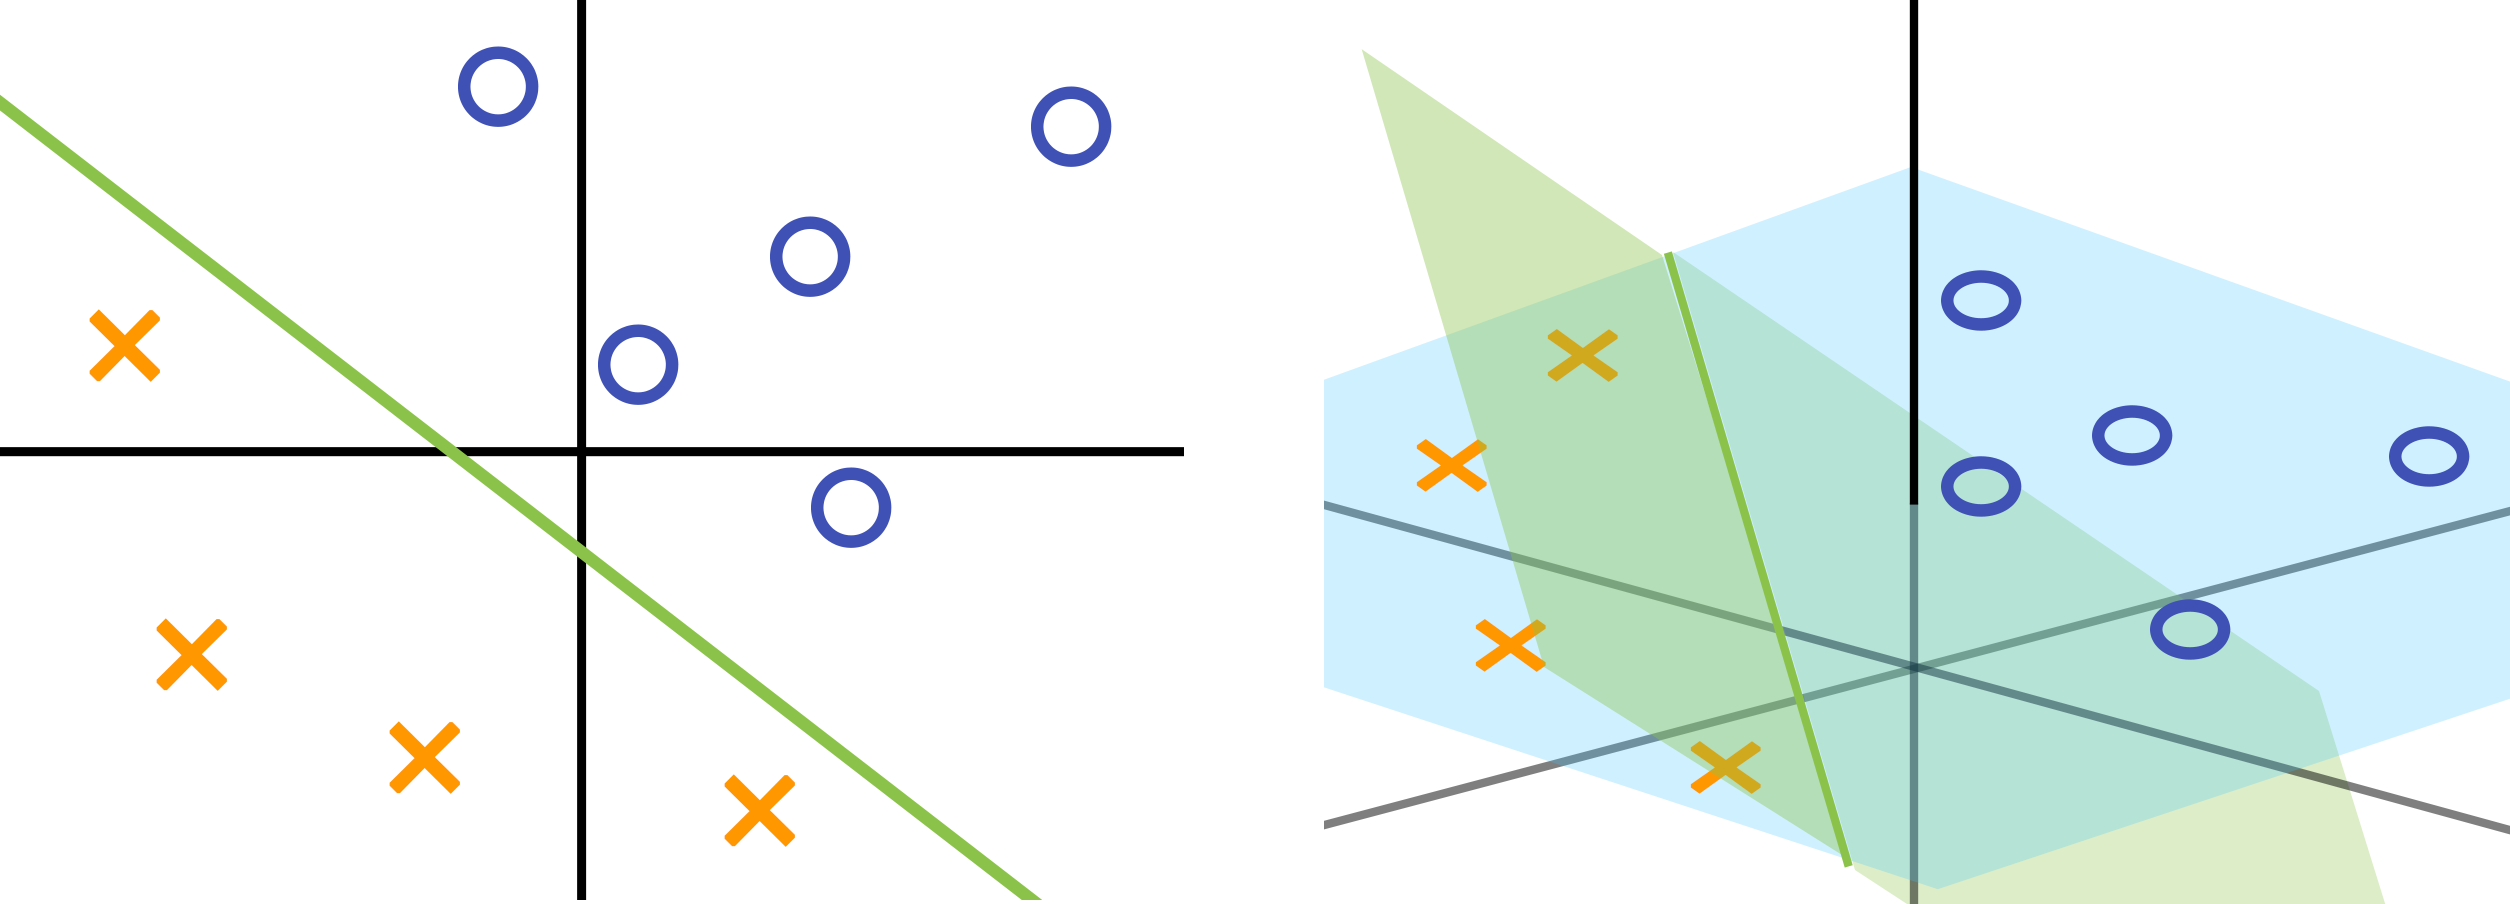
\includegraphics[height=1.8in]{8.png}
\end{center}

We'll abuse notation by dropping primes, assuming that $x$ is already augmented, and using $d$ as the new dimension. Suppose we now have $n$ inputs $(x_1, y_1), \ldots, (x_n, y_n)$. The linear regression is given by the $\beta$ that minimizes the sum of the square loss\[
  L(\beta) = \sum_{i=1}^n \left(y_i - f(x_i)\right)^2 = \sum_{i=1}^n\left(y_i - \beta^Tx_i\right)^2.
\]
Let $X$ be the $n \times d$ matrix $\bm{x_1 & \cdots & x_n}^T$. Note that we have the $x_i$ as \textit{rows} and not columns. Similarly let $Y$ be the $n \times 1$ matrix $\bm{y_1 & \cdots & y_n}^T$. Then the square loss is\[
  L(\beta) = (Y - X\beta)^T(Y - X\beta) % (Y - X\beta) = (n \times 1) - (n \times d)(d \times 1)
\]
Differentiate with respect to $\beta$ and set equal to zero to get\[
  \frac{\partial L}{\partial \beta} = -2X^T(Y - X\beta) = 0 \implies \beta = (X^TX)^{-1}X^TY, % (\beta) = (d \times n)(n \times d)(d \times n)(n \times 1)
\]
assuming $X^TX$ is invertible. We'll talk about how to deal with non-invertability later.

How do we use this for classification? It's mostly the same setup. Say that we each of the $x$s are classified into $k$ different classes. Then $y$, instead of being a scalar, will now be a $k$-dimensional vector $y = (y_1, y_2, \ldots, y_k)^T$, where $y_i = 1$ if $x$ is of category $i$, and $0$ otherwise. Then $Y$ would be an $n \times k$ matrix instead. The steps are exactly the same; in the end, we get $\beta$, which is a $d \times k$ matrix.
\begin{exrboxed}
  Check that if we replace $Y$, then the dimensions still work out.
\end{exrboxed}
So let's say we have a new input $x$ that we want to classify. We compute $f(x) = \beta^Tx$, then take the largest coordinate of $f(x)$ and classify it there.
\begin{exrboxed}
  One possible interpretation of $f(x)$'s coordinates are probabilities: the $i$th coordinate represents our probability that $x$ is in the $i$th category. Show that the sum of $f(x)$'s coordinates is $1$, assuming we've augmented $x$. Convince yourself that sometimes, the coordinates can be negative, or greater than $1$.
\end{exrboxed}
\vspace{-1em}
\begin{exrboxed}
  Given the matrix $\beta$, how do you find the decision boundary between the categories $i$ and $j$?
\end{exrboxed}

\subsubsection*{Regularization}

Non-invertibility is an actual issue. Even the matrix $X^TX$ being \textit{close} to non-invertible can cause problems due to numerical stability.

To deal with non-invertibility, we add a \textbf{regularization} term to the loss function. Intuitively, it acts as a penalty for $\beta$ being too ``complicated'', but for now, it simply fixes the non-invertible problem. The new loss function is now\[
  L(\beta) = \sum_{i=1}^n \left(y_i - f(x_i)\right)^2 + \lambda\norm{\beta}^2.
\]
Here, $\lambda$ is a hyperparameter. For small values of $\lambda$, it's similar to normal regression. As $\lambda$ grows, it pushes $\beta$ to be smaller. This turns it from linear regression, to an algorithm we call \textbf{ridge regression}.
\begin{exrboxed}
  Check that the $\beta$ that minimizes this is $(X^TX + \lambda I)^{-1}X^TY$. This is nice, because for $\lambda > 0$, $X^TX + \lambda I$ is always invertible.
\end{exrboxed}
In practice, matrix inversion is expensive and numerically unstable, so we usually minimize the loss function using \textbf{gradient descent}. We'll talk about gradient descent more when we get to neural networks.

\subsubsection*{Issues with linear regression}

Linear regression is a reasonable approach sometimes. But one big problem with naive linear regression is \textbf{masking}. If we try to use linear regression on the data below, which is in three categories, we get a decision boundary that completely masks the center one:

\begin{center}
  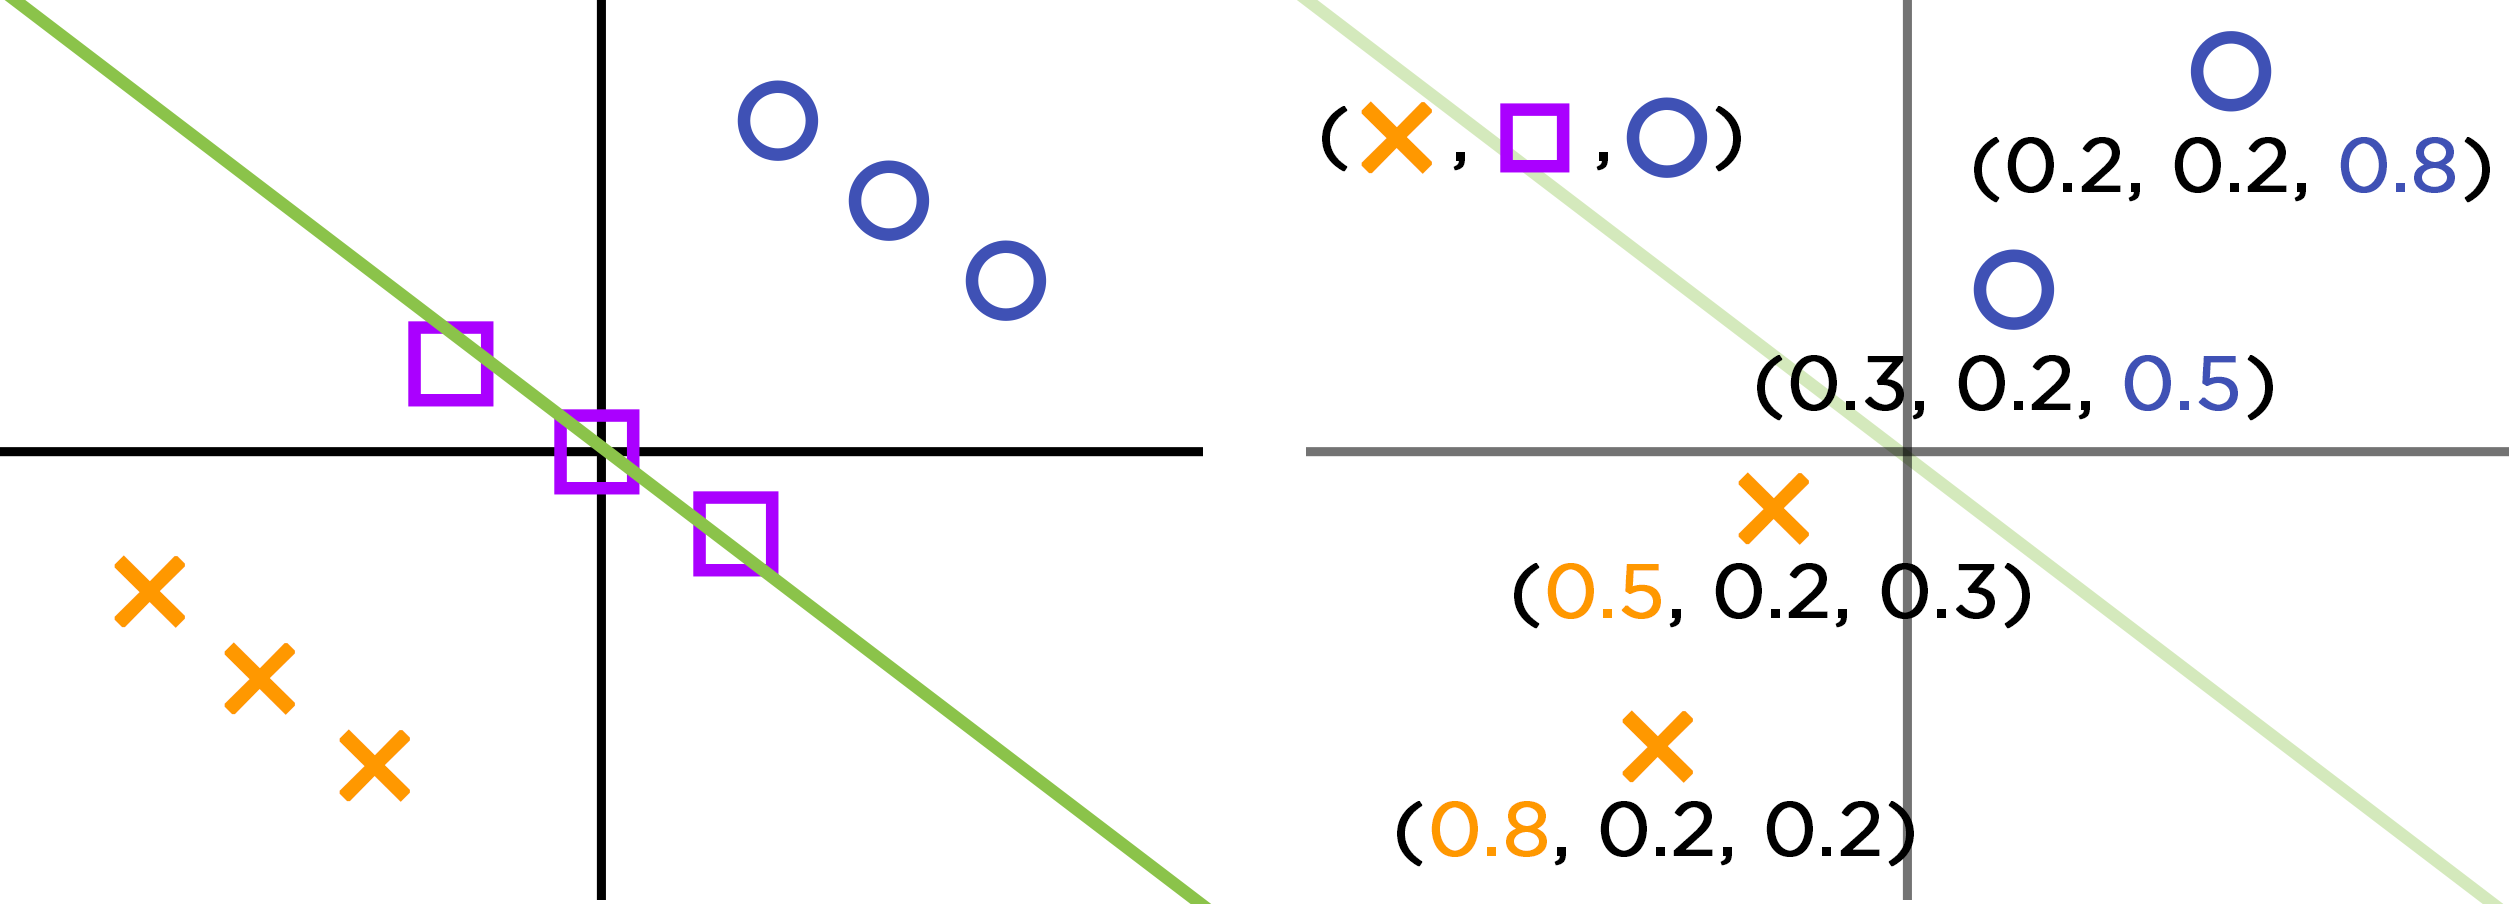
\includegraphics[height=1.8in]{9.png}
\end{center}

The problem is that the center coordinate is never large enough for it to be classified there. As we go from the lower-left to the top-right, $f(x)$'s center coordinate remains constant, and it's masked by the bottom and top coordinates. The figure above shows some samples of $f(x)$ at different points $x$.

In some sense, this issue arises because there isn't much theoretical justification for using linear regression on a classification problem. When we try to interpret the coefficients as probabilities, we don't get anything nice, other than the fact they all add up to $1$.

\subsubsection*{Other linear classifiers}

A more solid approach starts with Bayes's theorem:\[
  P(y = i \mid x) = \frac{P(x \mid y = i)P(y = i)}{P(x \mid y = 1)P(y = 1) + \cdots + P(x \mid y = k)P(y = k)}.
\]
In the case that $x$ is discrete, then we can estimate $P(x \mid y = i)$ by taking the ratio $P(x, y = i)/P(y = i)$ over the training data. This gives a \textbf{naive Bayes classifier}. In the case that $x$ is a vector, we'll model each of the $P(x \mid y = i)$ as a multivariate Gaussian:\[
  P(x \mid y = i) = \frac{1}{\sqrt{(2\pi)^d \Sigma_i}}\exp\del{-\frac{1}{2}(x - \mu_i)^T\Sigma_i^{-1}(x - \mu_i)}.
\]
We make the additional assumption that the $\Sigma$ are equal. Suppose we wanted to find the decision boundary between $P(y = i \mid x)$ and $P(y = j \mid x)$. We'll take the ratio, which conveniently cancels the denominator from Bayes's theorem: \[
  \frac{P(y = i \mid x)}{P(y = j \mid x)} = \frac{P(x \mid y = i)P(y = i)}{P(x \mid y = j)P(y = j)} = \frac{P(y = i)}{P(y = j)} \cdot \frac{\exp\del{-\frac{1}{2}(x - \mu_i)^T\Sigma^{-1}(x - \mu_i)}}{\exp\del{-\frac{1}{2}(x - \mu_j)^T\Sigma^{-1}(x - \mu_j)}}.
\]
Then we'll take the logartihm, which conveniently makes it linear: \[
  \log \frac{P(y = i \mid x)}{P(y = j \mid x)} = \log \frac{P(y = i)}{P(y = j)} - \frac{1}{2}\left(\mu_i + \mu_j\right)^T\Sigma^{-1}(\mu_i - \mu_j) + x^T\Sigma^{-1}(\mu_i - \mu_j).
\]
Then $P(y = i \mid x) > P(y = j \mid x)$ when this linear function is positive, and the other direction when it's negative. So this gives us a linear boundary between two classes. We then have to estimate $P(y = i)$, $\mu_i$, and $\Sigma$ from the data.

This is known as \textbf{linear discriminant analysis}. To the left is what it gives for the previous failed example for linear regression. To the right is what decision boundaries it gives on data that's actually produced by multivariate Gaussians:

\begin{center}
  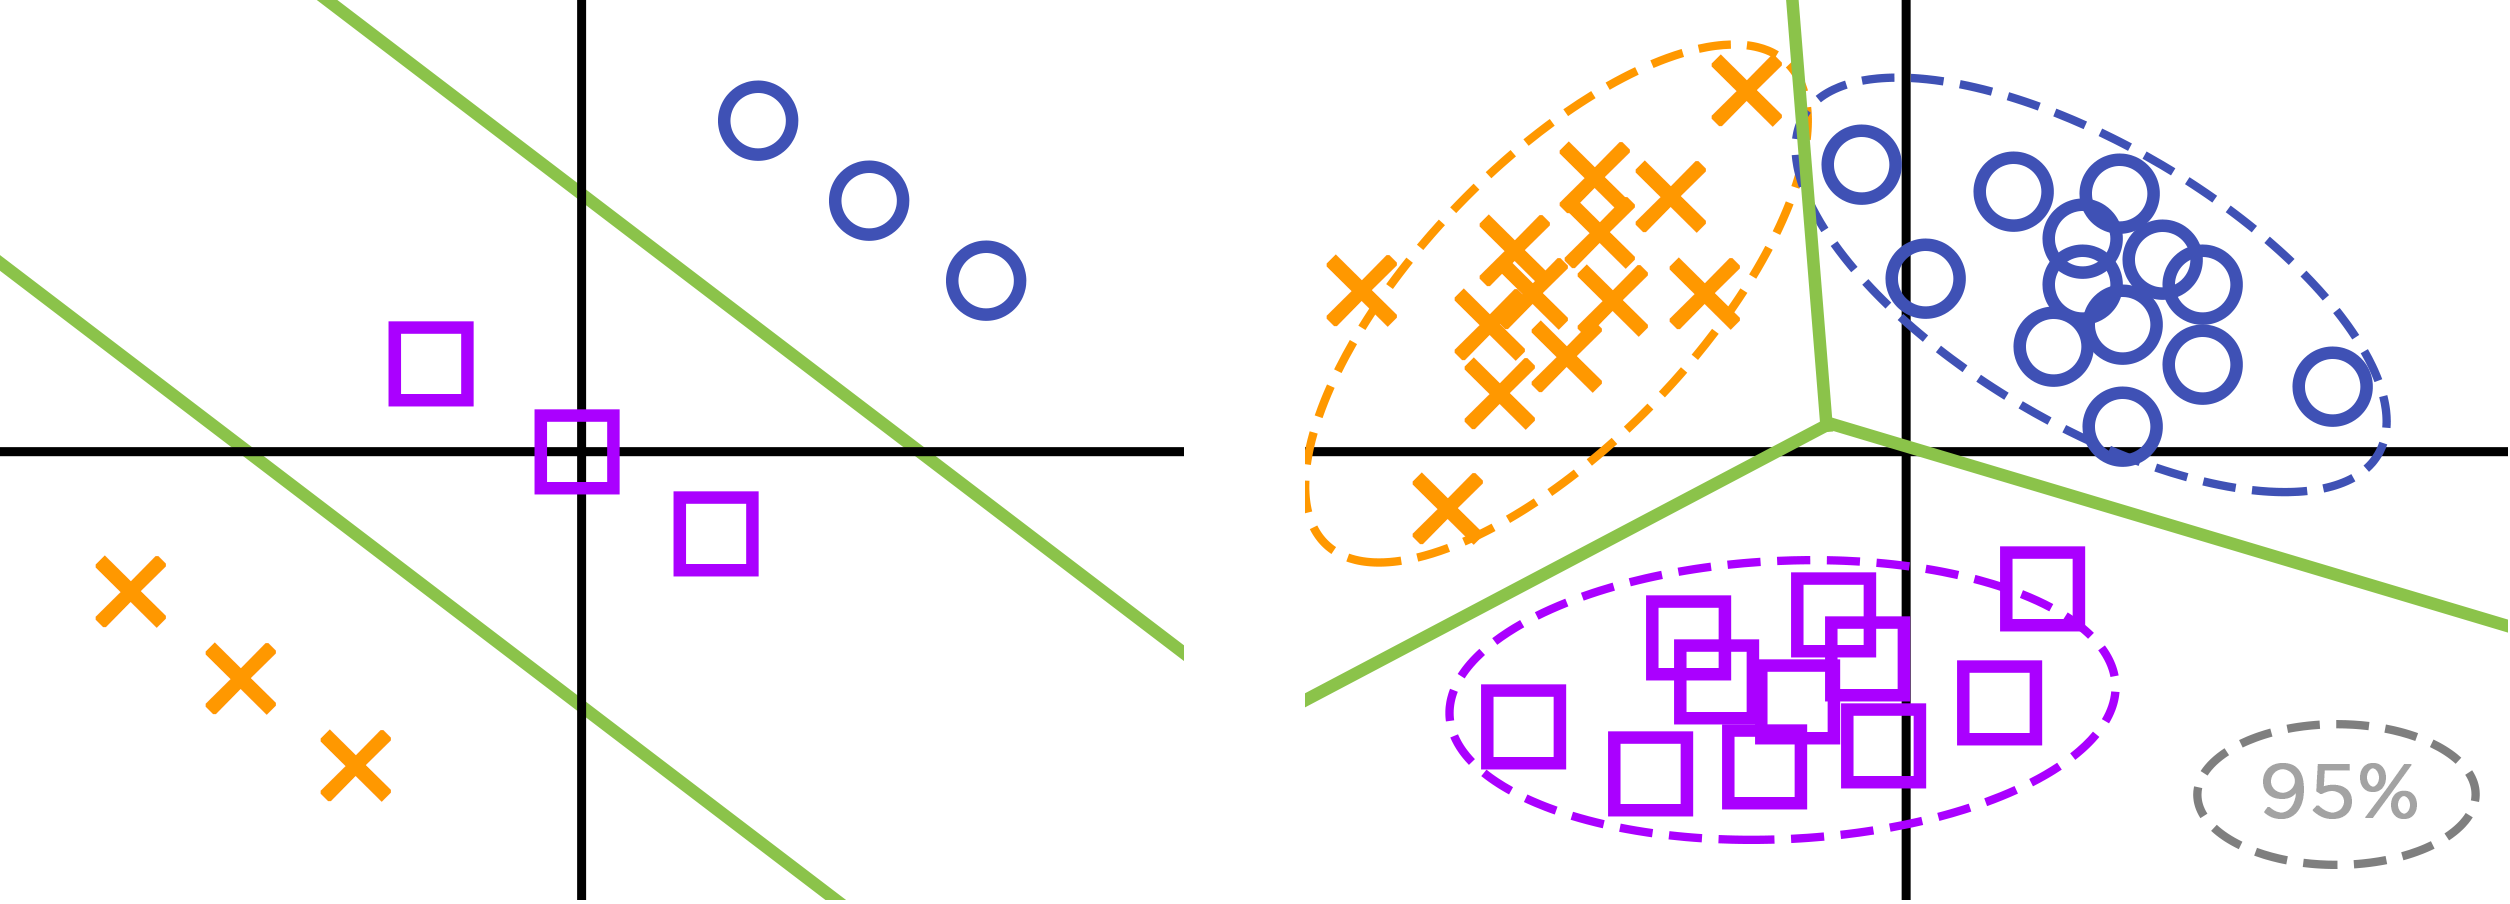
\includegraphics[height=1.8in]{10.png}
\end{center}

Another method, called \textbf{logistic regression}, starts directly by assuming that the log-ratios have a linear boundary, and then fitting directly from there. Logistic regression is generally safer than linear discriminant analysis, but both perform much better than linear regression in practice.

% gauss-markov?

\clearpage

\section{Non-linearity (July 25)}

\textit{Prerequisites:} Matrices, vectors, distances from points to planes, dot products. Nice, but not necessary: the previous seminar.

\subsubsection*{The perceptron}

For the rest of this seminar, I'll say \textit{plane} to mean hyperplane. Usually, in $d$-dimensional space, this refers to a $(d-1)$-dimensional hyperplane. So in two dimensions, this is just a line; in three dimensions this is a plane. We'll abuse notation by saying \textit{plane} to refer to its normal vector too.

Let's look at this data of circles and crosses in the plane. The nice thing about this data is that it's \textbf{linearly separable}. There's some plane that divides the data cleanly into the two classes.
\begin{center}
  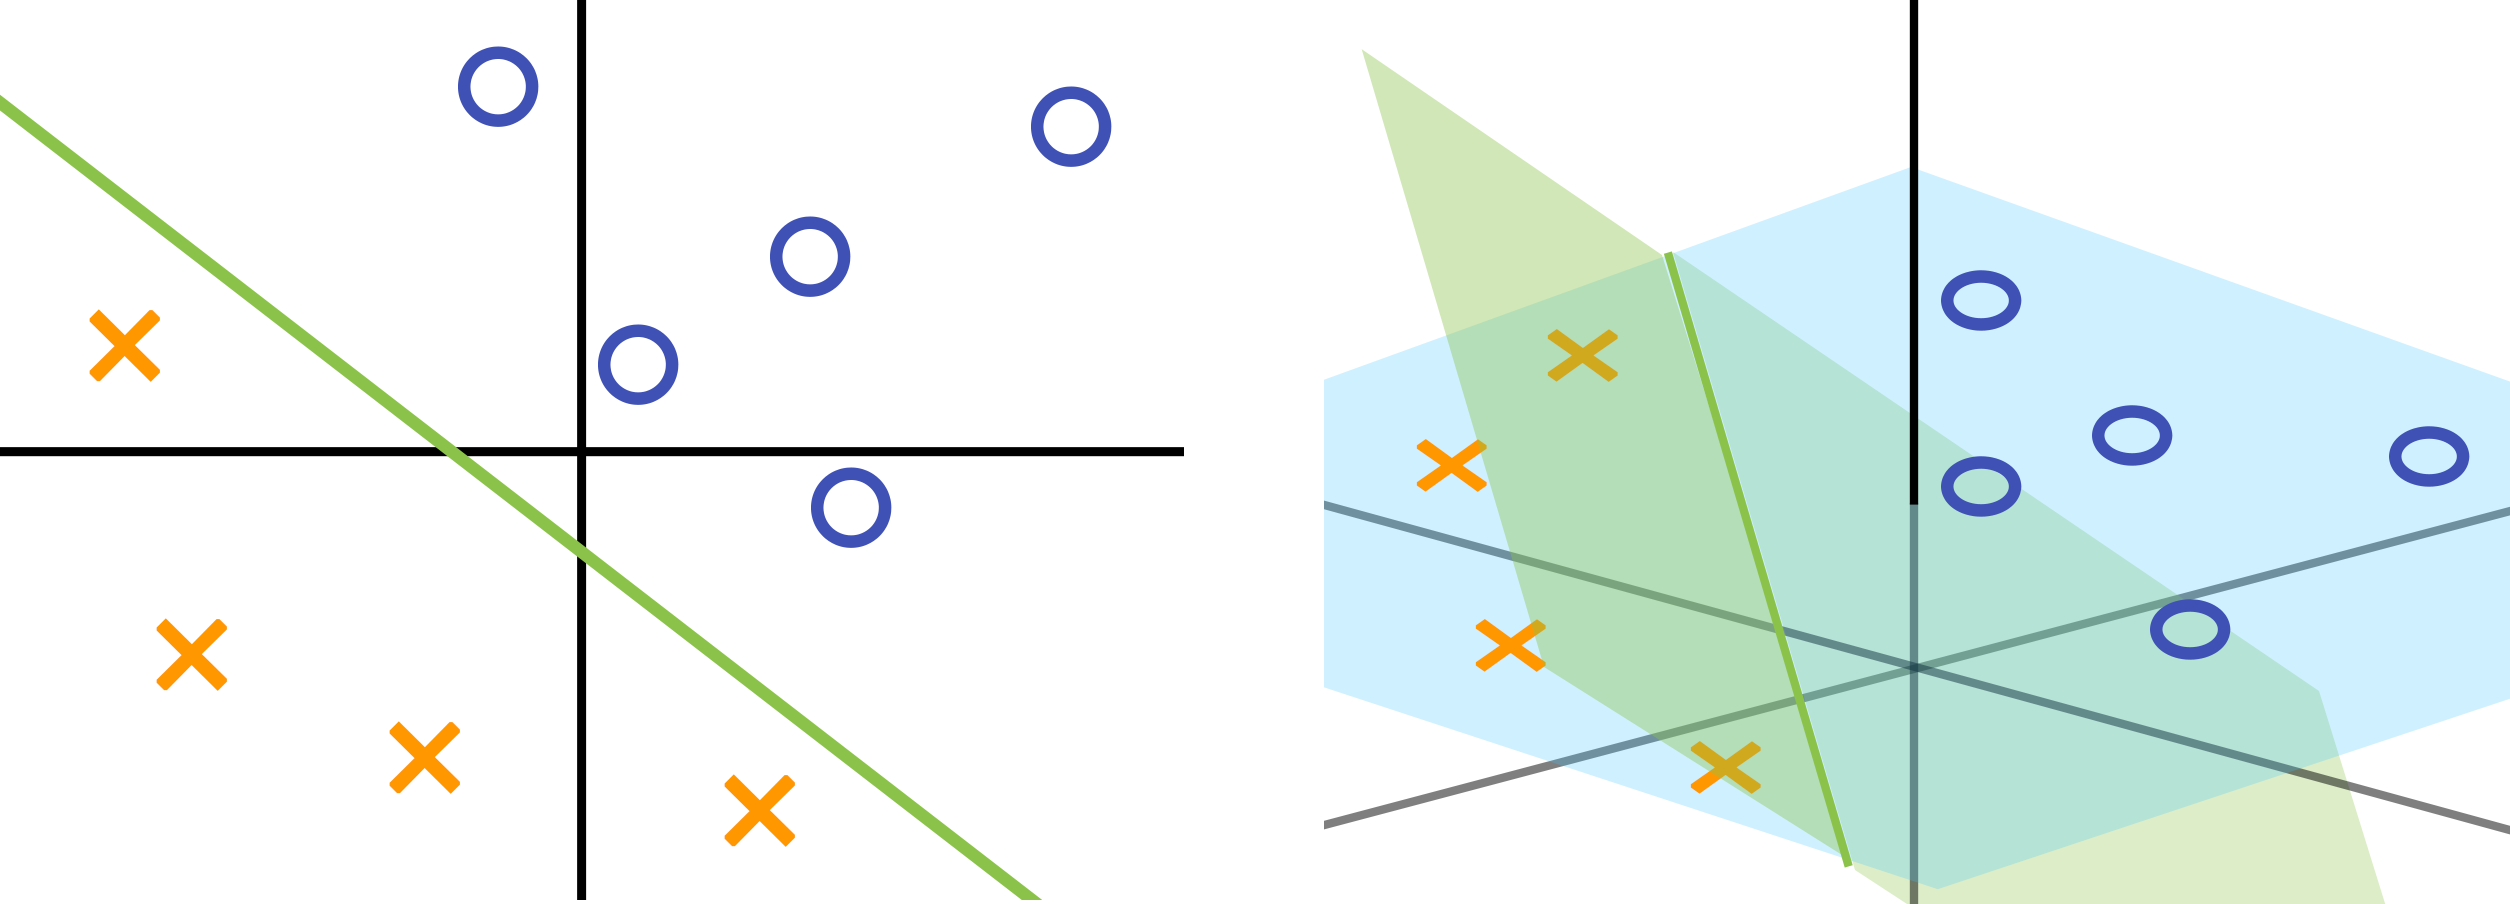
\includegraphics[height=1.8in]{11.png}
\end{center}
Recall how, in the previous seminar, we got rid of the constant term in the linear regression by adding a coordinate. The main idea is that we can rewrite a plane like $z = ax + by + c$ into $z = (a, b, c)(x, y, 1)^T$, which we can interpret as adding a new dimension, and it's just $1$ in that dimension. This is \textbf{projectivization}. Geometrically, it moves our points from the plane into space, and it turns our arbitrary plane into a plane passsing through the origin, as in the right figure above.

Planes passing through the origin as nice, because we can write them in the form $\beta^Tx = 0$, where $x$ is the vector of coordinates. Assuming our data has two classes, and is linearly separable, we're now going to introduce an algorithm, the \textbf{perceptron}, that finds such a separating plane.

Notation again. Our training data is $(x_1, y_1), \ldots, (x_n, y_n)$, in $d$-dimensional space, assuming we've already projectivized. We assume there are only two classes, and that each $y_i$ is either $-1$ or $+1$.

We're looking for the $d$-dimensional plane that separates the data. Let's say that we found such a plane, its normal vector is $\beta$, and $\beta$ points towards the $+1$ part of the data. Then we get $\beta^Tx > 0$ for the $x$ that's in the $+1$ side of space, $\beta^Tx < 0$ for the $x$ that's in the $-1$ side of space. In either case, if $(x, y)$ is a correctly classified example, then $y\beta^Tx > 0$. Keep this in mind.

The perceptron algorithm starts by setting $\beta = 0$. Then for $i = 1, 2, \ldots, n$, we check if $y_i\beta^Tx_i \le 0$. In other words, we check if $(x_i, y_i)$ is incorrectly classified. If it is, then we add $y_ix_i$ to $\beta$. We keep going through all points until everything's correctly classified.

\begin{exrboxed}
  Why does adding $y_ix_i$ make the classifier ``closer'' to being correct? If $y_i\beta^Tx_i \le 0$, what can we say about $y_i\left(\beta + y_ix_i\right)^Tx_i$?
\end{exrboxed}
\vspace{-1em}
\begin{exrboxed}
  Let's say we have two dimensional training data $D$, where the inputs are $x =(x_1, x_2)$. Further, let's say the $x_1$-coordinate ranges from $-1000$ to $1000$, while the $x_2$ coordinate ranges from $-1$ to $1$. Compare this to the $D'$, which is the same data, except $x_1$ is normalized to be within $-1$ to $1$. How do you think the perceptron algorithm will differ in these two cases?
\end{exrboxed}

\subsubsection*{Perceptron convergence}

The neat thing about the perceptron is that if a separating plane exists, it always finds it. The proof's actually pretty nice. The main idea is to take the ``best'' separating plane $\beta^*$, and show that the angle between $\beta$ and $\beta^*$ decreases fast enough.

Recall that the signed distance from a point $x$ to a plane $\beta$ is $\beta^Tx / \norm{\beta}$. This signed distance is positive if $x$ is in the side pointed to by $\beta$ and negative otherwise. So for an example $(x, y)$ that's correctly classified, the expression \[
  y \cdot \frac{\beta^Tx}{\norm{\beta}}
\]
is always positive, and it'll be negative otherwise. We call this the \textbf{margin} of the point. The margin of training data is the minimum margin over all points. With fixed training data, we abuse terminology and say the margin of the \textit{separator} too. So in this picture, one separating plane has a much smaller margin than the other. It should be ``intuitive'', in some sense, that a larger margin is better.
\begin{center}
  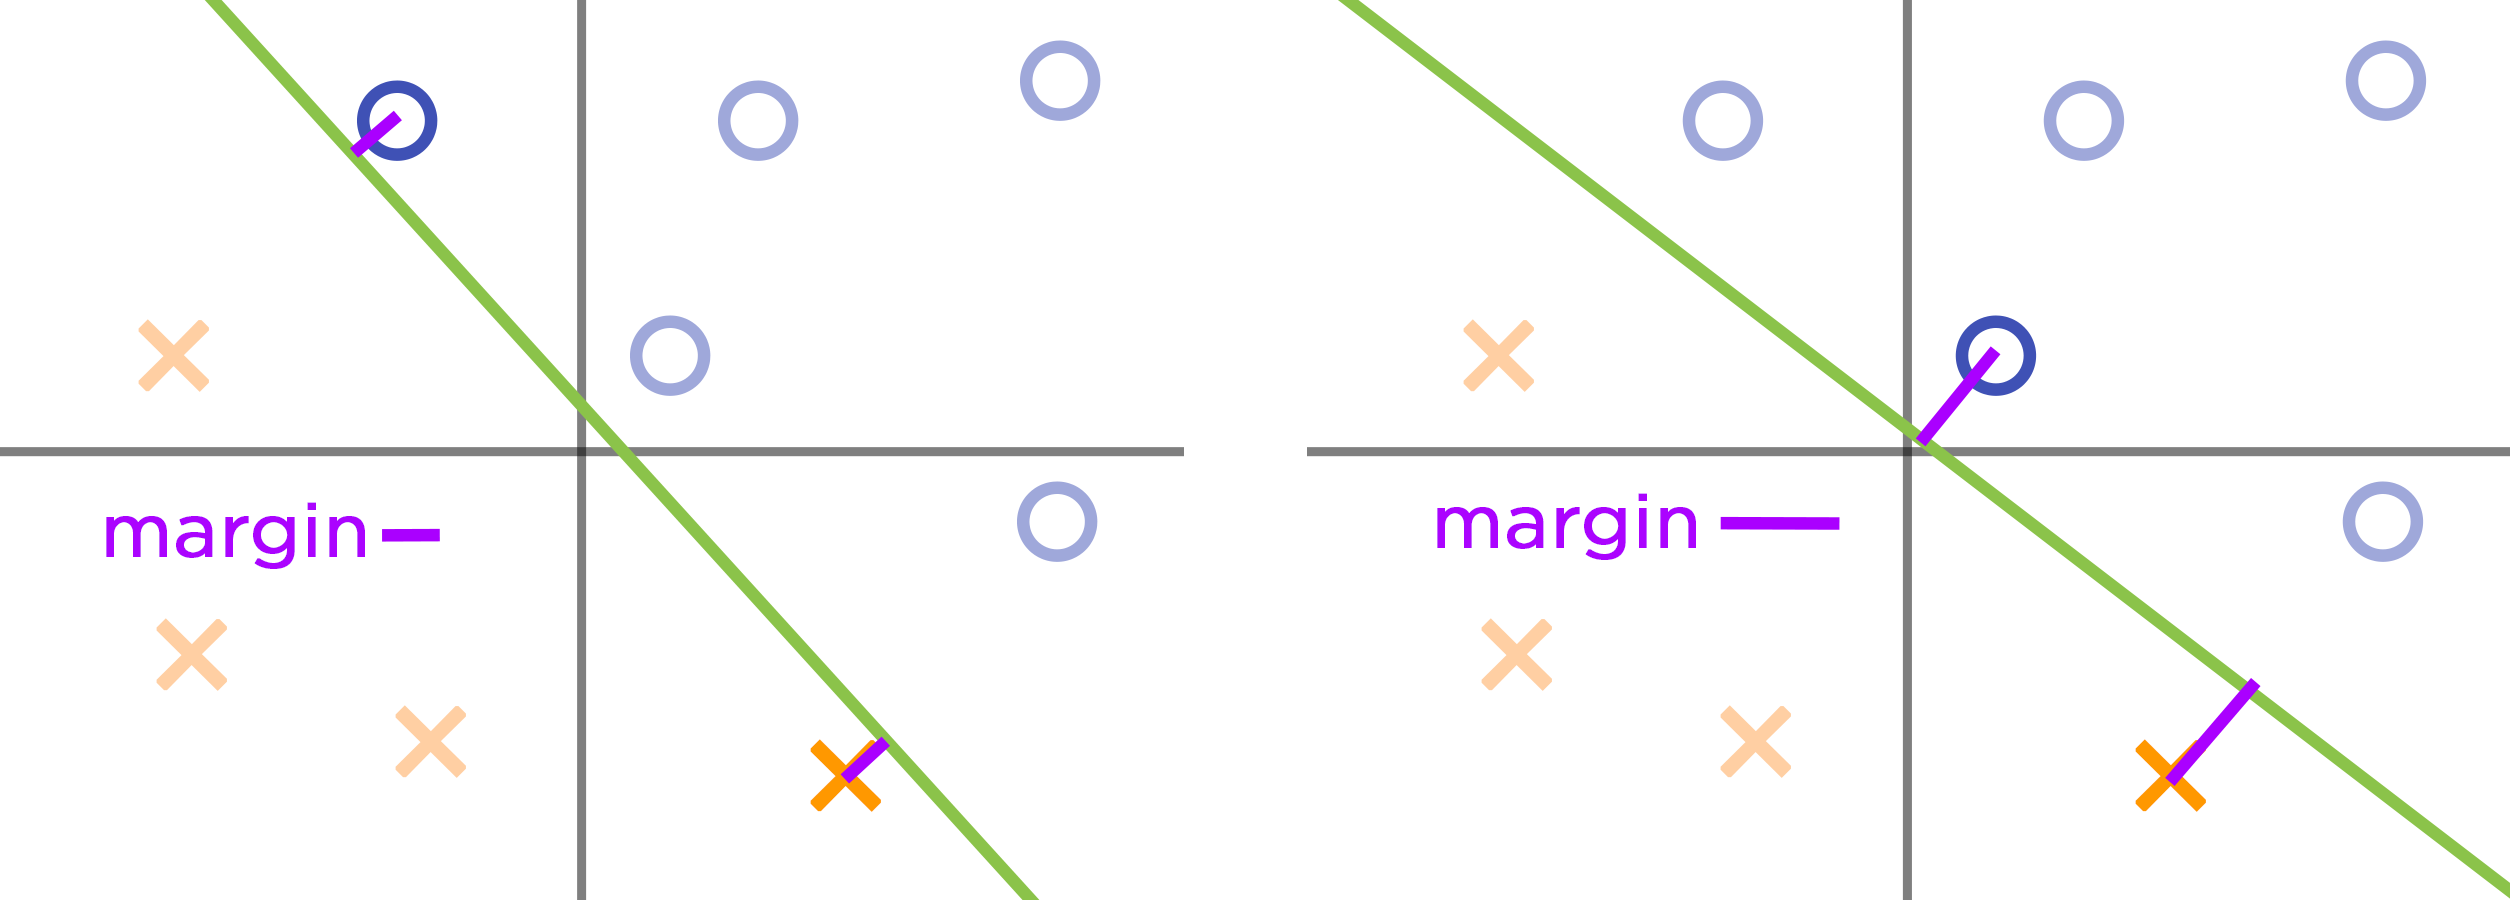
\includegraphics[height=1.8in]{12.png}
\end{center}
Now for the convergence theorem. We assume that the data has a separating plane; further assume that the separating plane $\beta^*$ has the margin $M$. And suppose that $R$ is the maximum of $\norm{x}$ over all the data. The key result is that the perceptron algorithm will make at most $(R / M)^2$ updates, and after that, it's going to be a separating plane.

Alright, the proof. Let $\beta_k$ be the separator after the $k$th update of the perceptron. We said we'd look at the angle between the two planes:
\[
  \cos\left(\beta_k, \beta^*\right) = \left(\frac{\beta_k \cdot \beta^*}{\norm{\beta^*}}\right)\left(\frac{1}{\norm{\beta_k}}\right).
\]
If the $k$th update happened on the point $(x, y)$, then we can bound the first factor using $\beta_{k-1}$:
\[
  \frac{\beta_k \cdot \beta^*}{\norm{\beta^*}}
  = \frac{\left(\beta_{k-1} + yx\right) \cdot \beta^*}{\norm{\beta^*}} \ge \frac{\beta^{k-1} \cdot \beta^*}{\norm{\beta^*}} + M,
\]
after distributing the dot product. Repeatedly do this until you get to $\beta_0 = 0$; this shows the first factor is at least $kM$.

For the second factor, since $(x, y)$ is classified incorrectly, then $y(\beta_{k-1}^Tx) \le 0$, meaning
\begin{align*}
\norm{\beta_k}^2 &=
\norm{\beta_{k-1} + yx}^2 \\
&= \norm{\beta_{k-1}}^2 + 2y\left(\beta_{k-1}^Tx\right) + \norm{x}^2 \\
&\le \norm{\beta_{k-1}}^2 + 2 \cdot 0 + R^2.
\end{align*}
Again, repeating until we hit $\beta_0$, we get the bound $\norm{\beta_k} \le R\sqrt{k}$. Hence
\[
  \cos\left(\beta_k, \beta^*\right) = \left(\frac{\beta_k \cdot \beta^*}{\norm{\beta^*}}\right)\left(\frac{1}{\norm{\beta_k}}\right) \ge kM \cdot \frac{1}{R\sqrt{k}} = \frac{M}{R}\sqrt{k}.
\]
As the maximum value of $\cos$ is $1$, we get $k \le (R / M)^2$. So any $k$ larger than this can't have had an update preceding it, which gives the bound.
\begin{exrboxed}
  How do we interpret this bound? How is the bound $(R / M)^2$ affected by scaling all the input coordinates of the training data? What about if we only scaled one coordinate?
\end{exrboxed}

\subsubsection*{Basis transformations}

While linear classifiers may seem pretty specific, there's a neat way to generalize them to make non-linear classifiers, using (non-linear) basis transformations. Consider the data on the left:
\begin{center}
  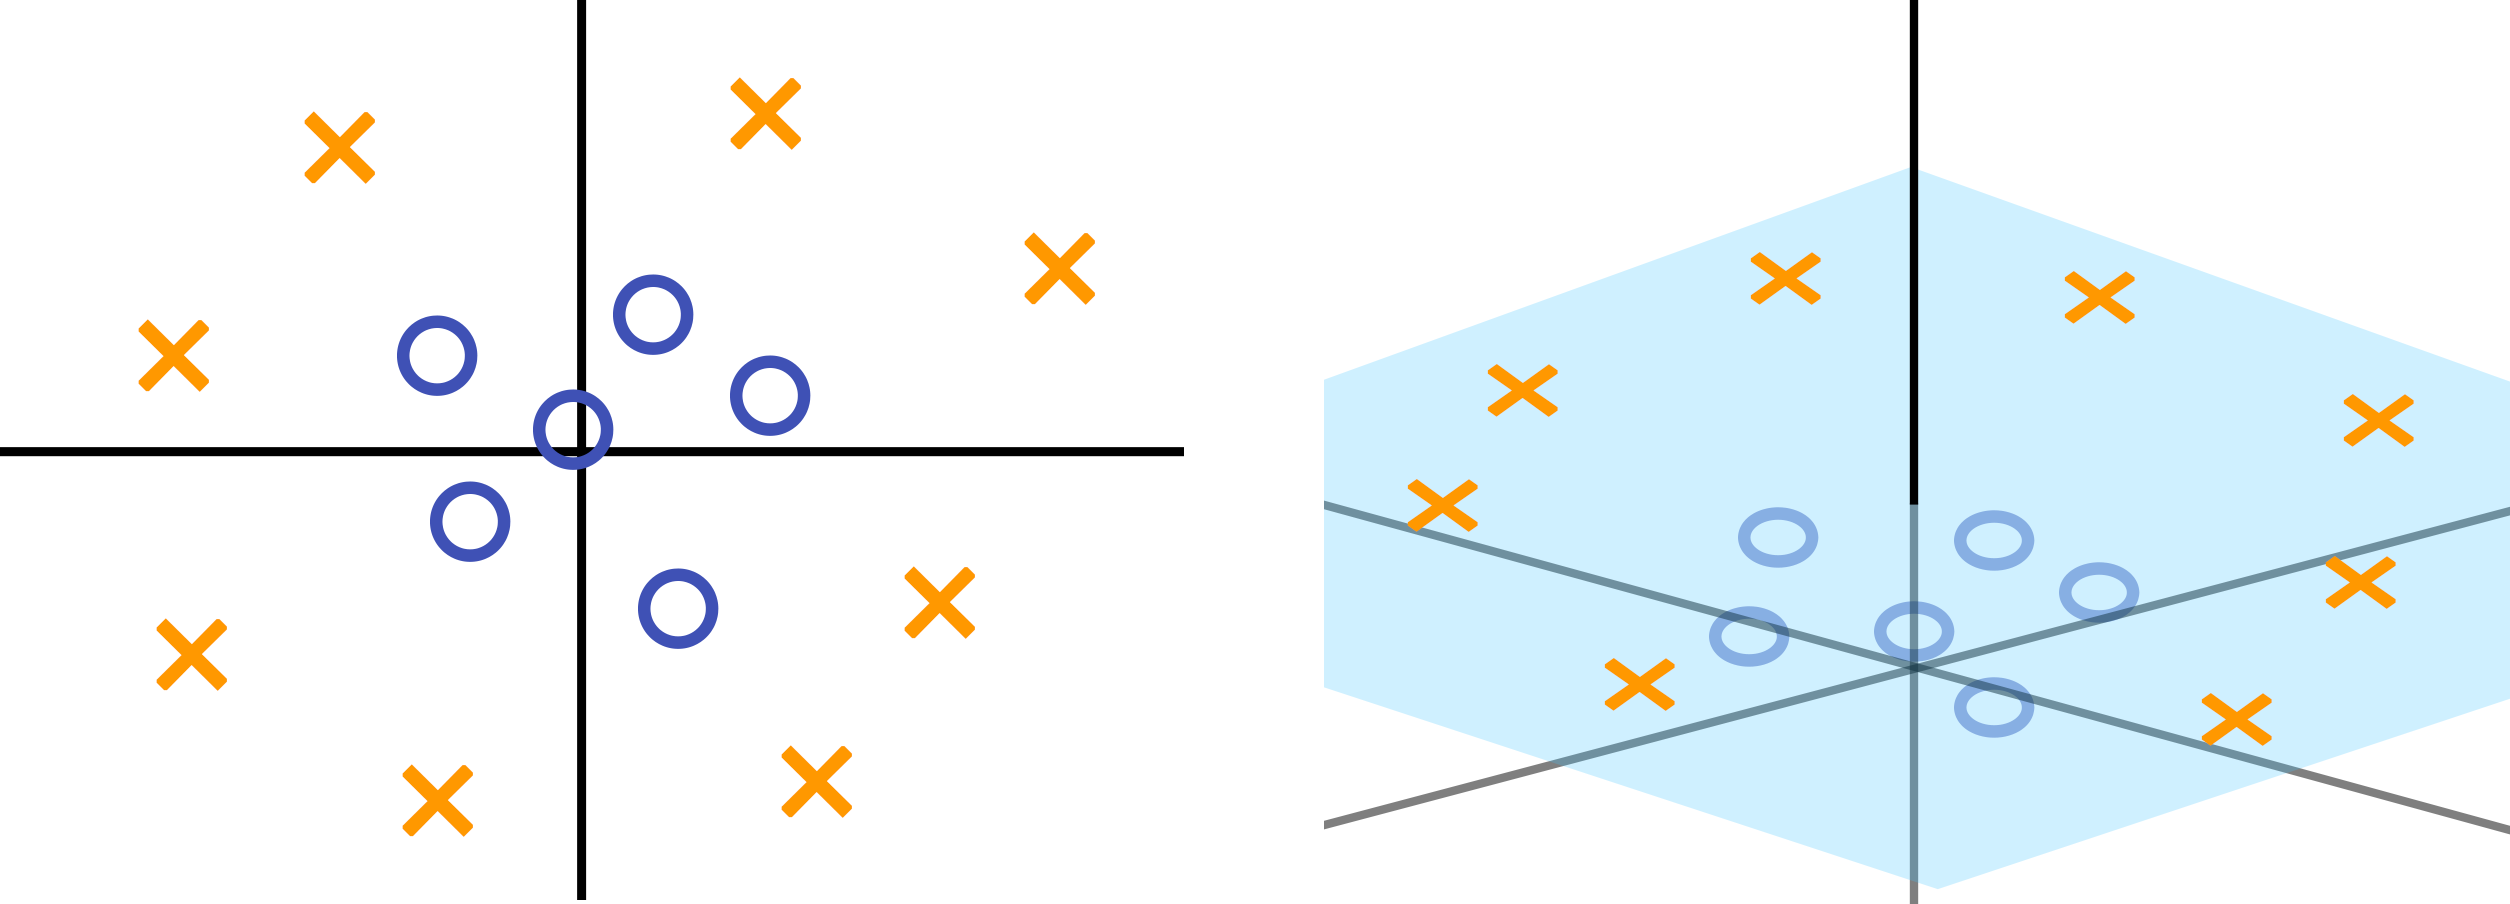
\includegraphics[height=1.8in]{13.png}
\end{center}
It's not linearly separable. But if we take the input $(x, y)$, and lift it by its distance to the origin, so that it becomes $(x, y, x^2 + y^2)$, all of a sudden it is! The plane that separates it is $z = k$, for some $k$. In the original space, this corresponds to $x^2 + y^2 = k$.

Of course, this feels like a cheat; we hand-crafted this transformation ourselves, didn't we? Is there a general, or \textbf{domain-independent} way to do this? One systematic way is to use the $k$th-order \textbf{polynomial basis}, which adds to the vectors all monomials of degree at most $k$. So the second-order transformation $\varphi$, for a two-dimensional point, would be \[
  \varphi: (x, y) \mapsto (1, x, y, x^2, y^2, xy).
\]
Here's the \textbf{XOR dataset}, which is a notorious dataset in twentieth-century machine learning. With the second-order polynomial transformation, the perceptron finds this separator after four updates. Note that it's a hyperbola---why?
\begin{center}
  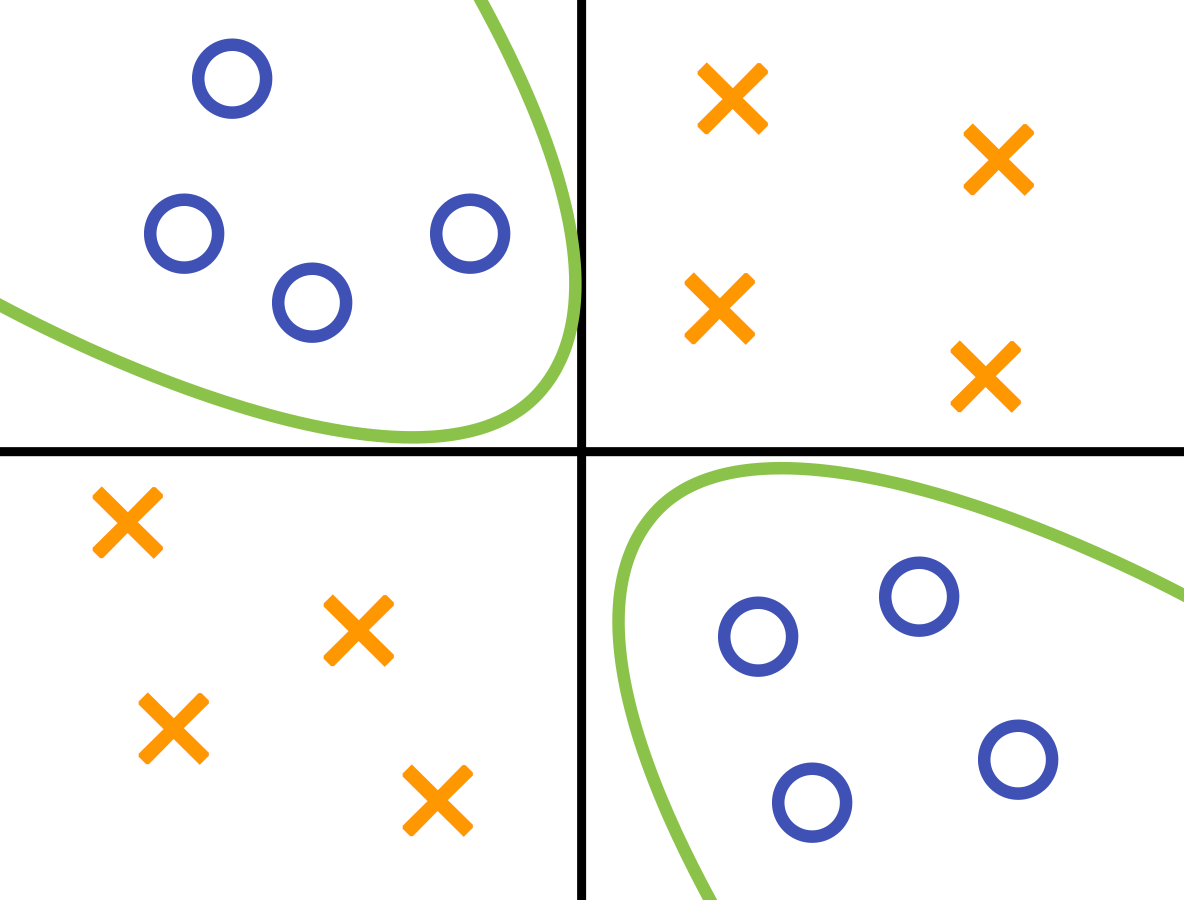
\includegraphics[height=1.8in]{14.png}
\end{center}

\subsubsection*{The kernel trick}

But even the polynomial basis is pretty constrained. There are two main issues with it. First, it's costly to compute the $k$th-order transform for any reasonable $k$ for \textit{every} example in the training data. And second, it's rather limiting. There's no easy way to generalize this to other non-linear transformations we might want to try.

We can solve both of these issues through what's called \textbf{the kernel trick}. We'll apply the kernel trick to the perceptron, and it'll involve two parts:
\begin{itemize}
  \item taking the \textit{dual perceptron}, which is really applying the concept of \textit{duality} from linear programming,
  \item then rewriting dot products using \textit{kernel functions}, which will implicitly map data into higher-dimensional space.
\end{itemize}

We'll start with the dual perceptron. Recall that every time we make a mistake with the point $(x, y)$, we update $\beta$ to be $\beta + yx$. Now consider what this looks like \textit{in total}. Let's say our training set is $(x_1, y_1), \ldots, (x_n, y_n)$, and that we made a mistake on the $i$th point $\alpha_i$ times. Then \[
  \beta = \alpha_1y_1x_1 + \cdots + \alpha_ny_nx_n.
\]
Now, how do we classify a new point, $x$? We take $\beta^Tx$ and look at the sign. But this is just \[
  \beta^Tx = \alpha_1y_1(x_1 \cdot x) + \cdots + \alpha_ny_n(x_n \cdot x).
\]
We've removed dependence on $\beta$ now, and written the problem entirely in terms of the vector $\alpha = (a_1, \ldots, \alpha_n)$. This gives us the \textbf{dual perceptron}: rather than storing $\beta$, we store $\alpha$. To run the dual perceptron algorithm, we start with $\alpha = 0$, compute the above sum, and if the sign is wrong, we change the corresponding coordinate of $\alpha$.
\begin{exrboxed}
  If you're familiar with duality in linear programming, how is this related to that?
\end{exrboxed}

And now, we're going to rewrite the dot products $x_i \cdot x$ with \textbf{kernel functions}, $K(x_i, x)$, which take two $d$-dimensional vectors and gives a scalar. This gives us \[
  \alpha_1y_1K(x_1, x) + \cdots + \alpha_ny_nK(x_n, x).
\]
The idea is that a kernel function represents the inner product in a higher-dimensional space. For example, consider the kernel function \[
  K\left((x, y), (x', y')\right) = \left(1 + (x, y) \cdot (x', y')\right)^2.
\]
This expands to \[
  1 + 2xx' + 2yy' + x^2x'^2 + y^2y'^2 + 2xyx'y'.
\]
Now consider the transformation $\varphi: (x, y) \mapsto (1, x\sqrt{2}, y\sqrt{2}, x^2, y^2)$. Then \[
  K\left((x, y), (x', y')\right) = \varphi(x, y) \cdot \varphi(x', y'),
\]
where the outer dot product is in the higher-dimensional space. So this generalizes our polynomial transformation into looking for kernel functions instead.

Kernel functions represent not only polynomial transformations, but also things like $-\exp\left(k\norm{x - x'}\right)^2$, a radial basis. Later, we'll see that neural networks can be thought of as using the kernel function $\tanh\left(k_1 x \cdot x' + k_2\right)$. Such kernel functions are usually required to be positive definite symmetric, so that they map to the inner product of some higher-dimensional space. (Something something linear algebra.)

\subsubsection*{Support vector machines}

Recall that the perceptron is guaranteed to find a separating plane, assuming that the data is linearly separable. There are two issues here. First, there is no guarantee on how \textit{good} this separating plane is. It could very well be a plane with a really low margin. And second, there are no guarantees at all if the data \textit{isn't} linearly separable; even just one outlier can throw off the whole algorithm.

Both of these issues are covered by \textbf{support vector machines}. In the separable case, SVMs find the separator with the maximum margin, and it generalizes to the non-separable case as well.

Recall that the margin of a point $(x, y)$, with respect to the plane $\beta$, is $y \beta^T x / \norm{\beta}$. This represents the distance of the point to the plane. We can treat finding the maximum margin separator as an optimization problem now:
\[
  \text{maximize }M \text{ if } y_i \cdot \frac{\beta^Tx_i}{\norm{\beta}} \ge M \text{ for }i = 1, 2, \ldots, n.
\]
Note that if $\beta$ satisfies the inequality, then any positive multiple of $\beta$ satisfies it too. We can thus fix $\norm{\beta} = 1/M$, which makes the problem
\[
  \text{minimize }\norm{\beta} \text{ if } y_i\beta^Tx_i \ge 1 \text{ for }i = 1, 2, \ldots, n.
\]
Solving this problem would find the maximum margin separator. To deal with the outliers, we're going to add \textbf{slack variables}. Unfortunately, it is standard notation to write these as $\xi_1, \ldots, \xi_n$:
\[
  \text{minimize }\norm{\beta} \text{ if } y_i\beta^Tx_i \ge 1 - \xi_i \text{ for }i = 1, 2, \ldots, n.
\]
These measure how ``badly classified'' each individual point is: $\xi_i$ is $0$ if it's correctly classified, and if it's positive, it's proportional to the distance ``across the wrong side'' of the classifier:
\begin{center}
  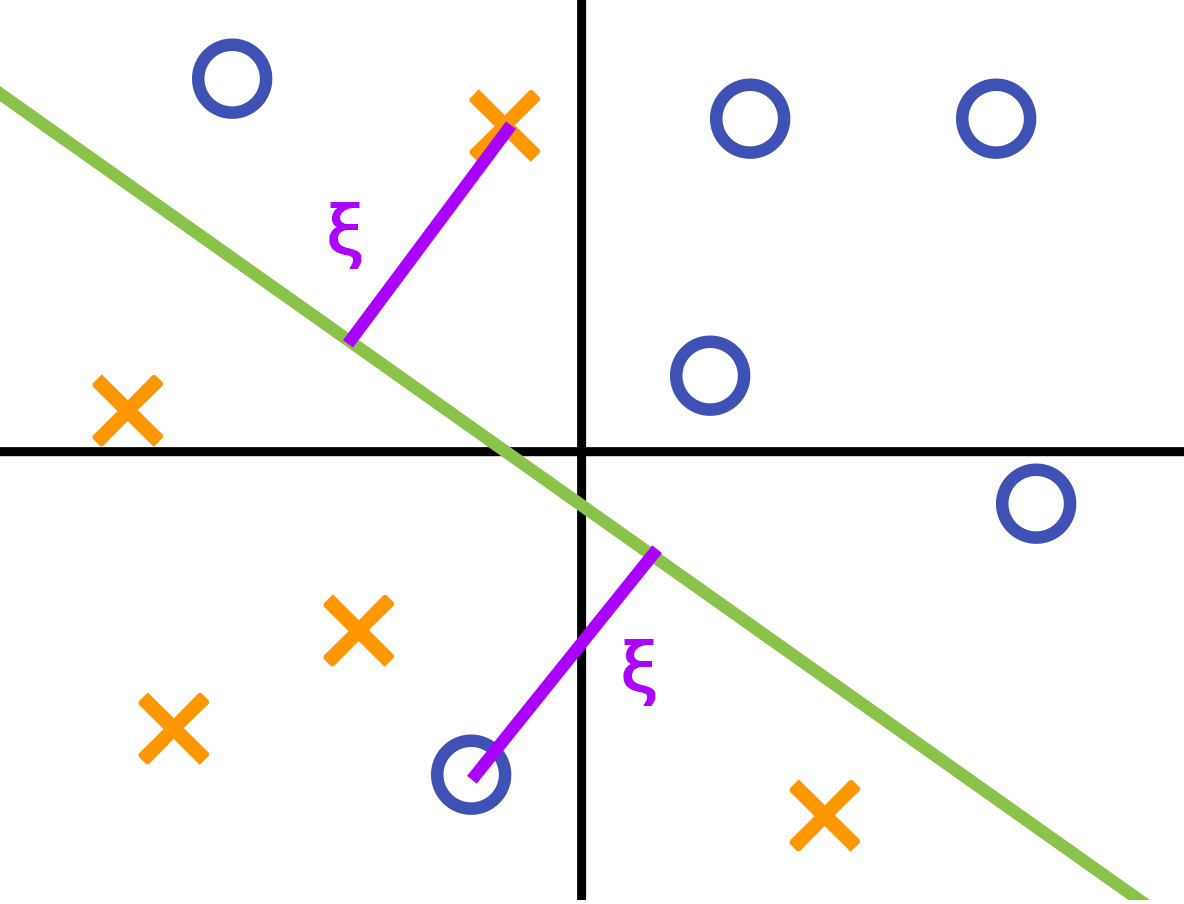
\includegraphics[height=1.8in]{15.png}
\end{center}
By allowing some fixed amount of slack, usually with the constraint $\xi_1 + \cdots + \xi_n \le$ some fixed constant, we can allow some amount of misclassification.

The SVM algorithm is independent of the technique used to solve this optimization problem. Traditionally, this is solved by taking the dual problem, then applying quadratic programming. Like the perceptron, the dual problem is only written in terms of dot products, so you can use the kernel trick. I don't think the algebra's very instructive so I won't include it here.

More recently, this optimization is solved using techniques like \textbf{gradient descent}. We won't go through what gradient descent is now, but it's a useful technique to solve minimization problems that we'll encounter again when we talk about neural networks.

\clearpage

\section{Generalization (August 1)}

\textit{Prerequisites:} Bayes's theorem, the first seminar. Nice, but not necessary: the second seminar.

\subsubsection*{Occam's razor}

So far, we've discussed several methods to solve the classification problem, from $k$-nearest neighbors, to linear regression, to linear discriminant analysis, to the perceptron, to support vector machines. We can keep going and talk about more classifiers, which we'll do next time when we talk about neural networks. But I think it's also useful to talk about some more bigger picture things.

One perspective of machine learning is that the key problem is the problem of \textbf{induction}, or the problem of \textbf{generalization}. How well does a learning algorithm perform on new data, given the data it already knows?

Occam's razor says that, when presented with several hypotheses that fit the data, the simplest explanation is most likely correct. To see how it applies to machine learning, consider how the choice of $k$ affects the decision boundaries for $k$-nearest neighbors in this data, from $k = 1$, to $3$, to $50$.

\begin{center}
  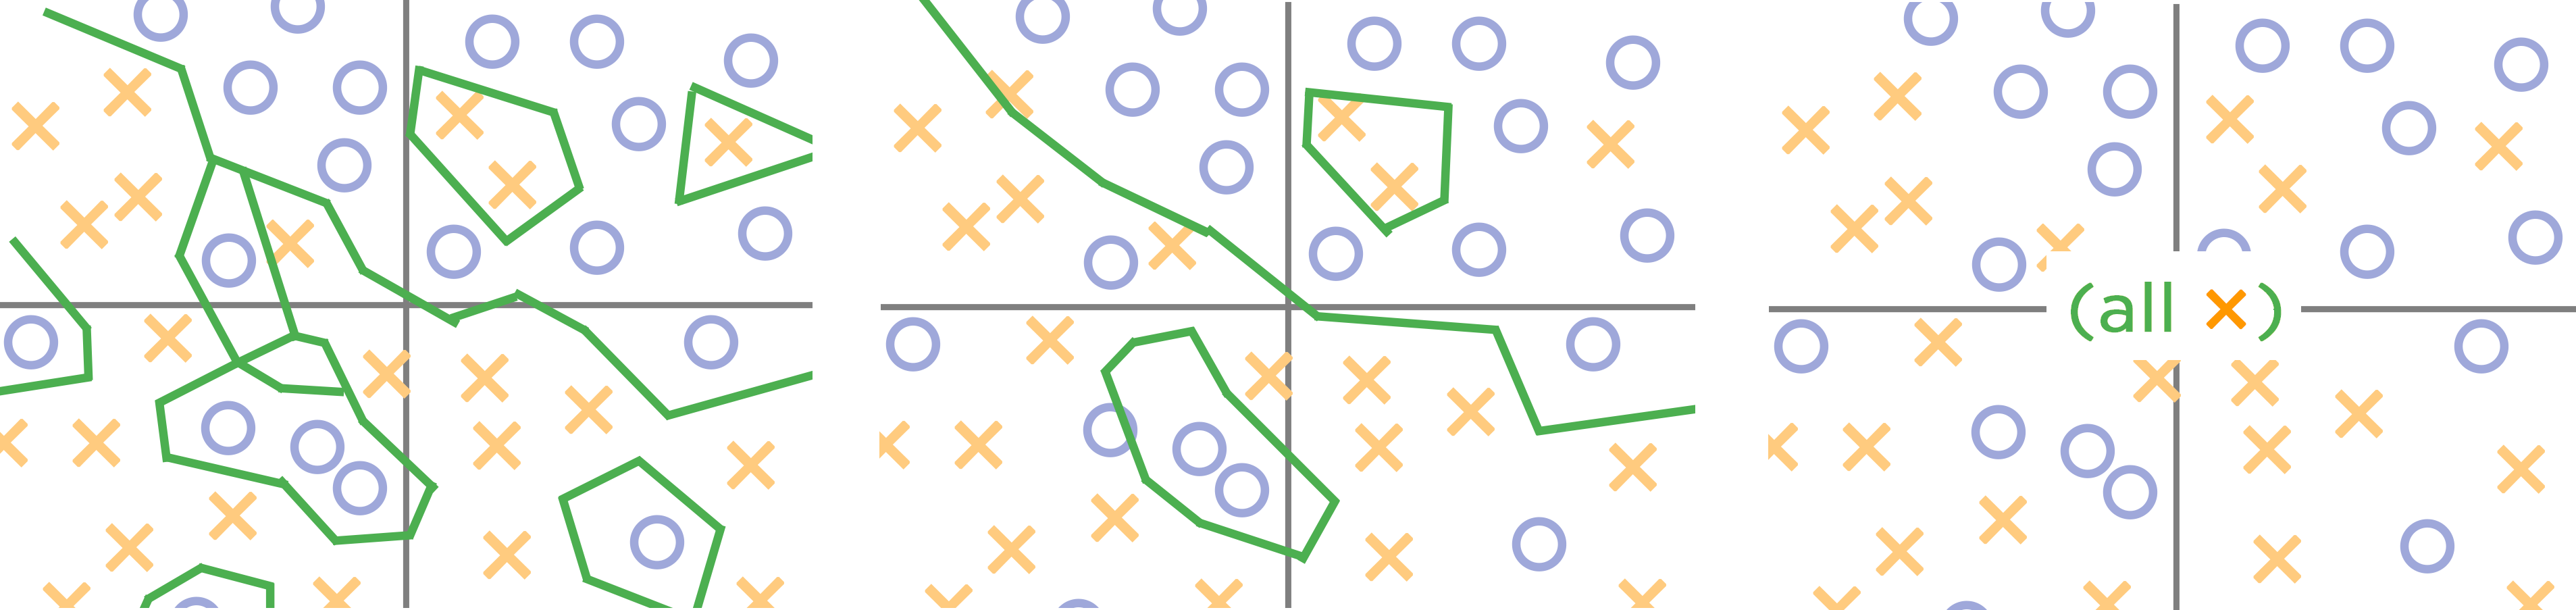
\includegraphics[width=\textwidth]{16.png}
\end{center}

Or consider something like polynomial interpolation. Here's some data, where we find the best-fitting polynomial of degree $d$, or the one that minimizes the sum of squared errors. See how the choice of $d$, from $1$ to $2$ to $6$, affects the model:

\begin{center}
  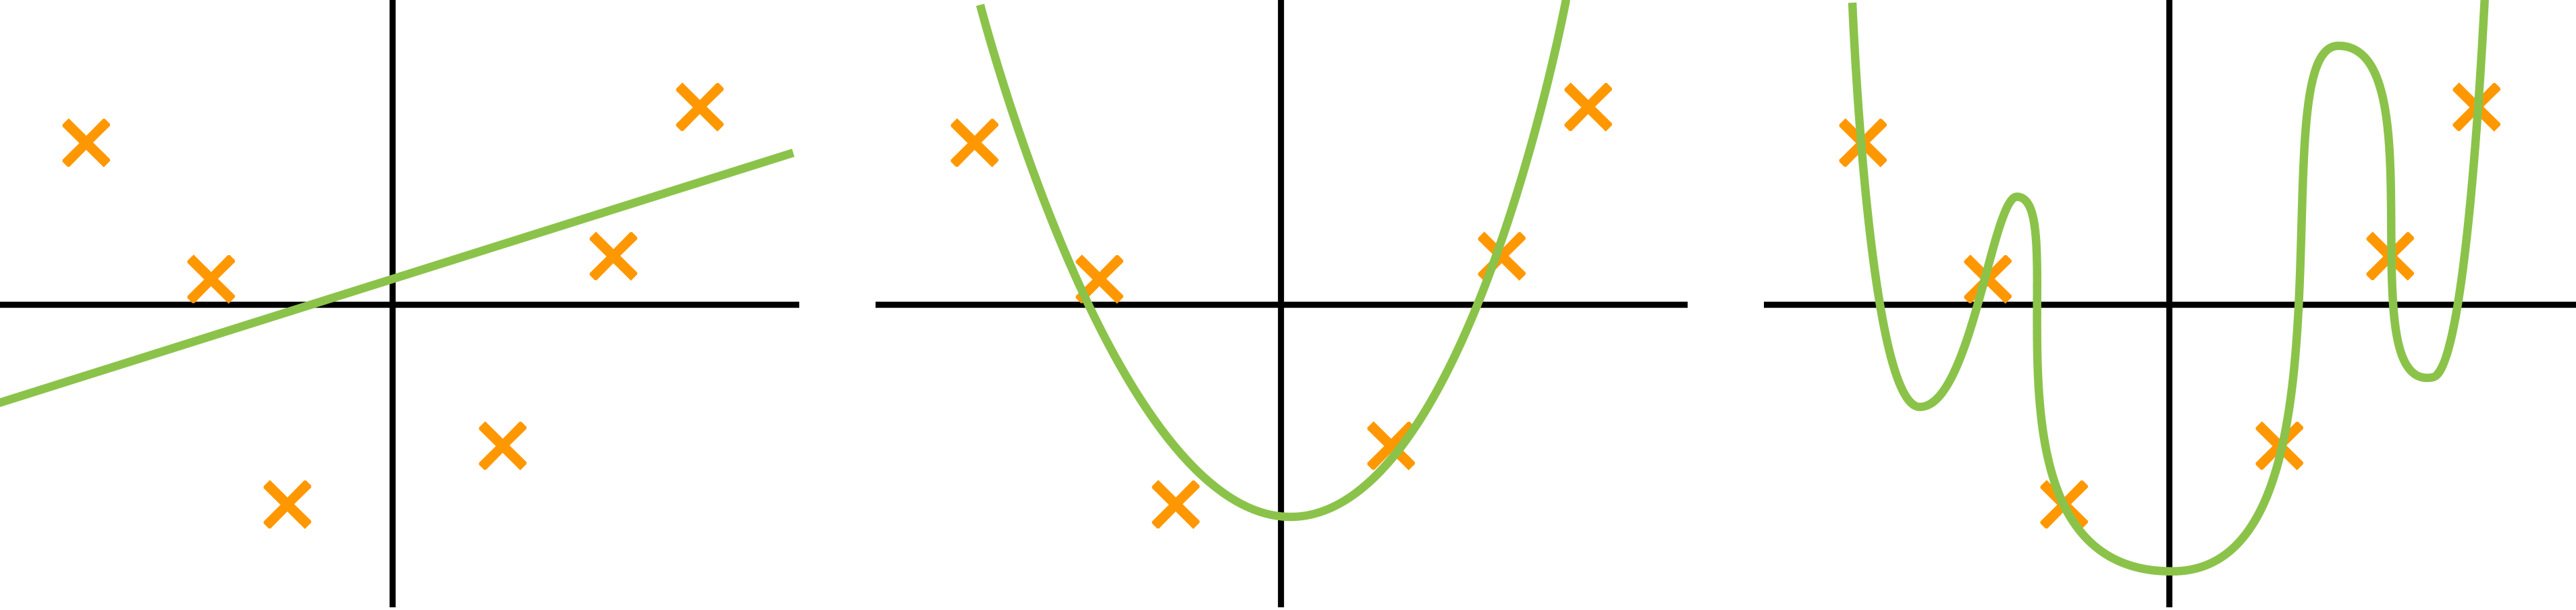
\includegraphics[width=\textwidth]{17.png}
\end{center}

Certainly you wouldn't want your hypothesis to be too complex. That's \textbf{overfitting}: the issue you get when your hypothesis fits too closely to the existing data, so much that it wouldn't perform well on future data. And this fits in with Occam's razor, which tells us that we should pick simpler hypotheses, rather than more complex ones.

But there's another side to Occam's razor. You don't want your model to be too simple either, because then you risk not fitting the data well at all. That's \textbf{underfitting}: when your model isn't complex enough to capture the structure of the existing data.

The balance between underfitting and overfitting go hand-in-hand. Today's talk is about the various ways this idea appears in machine learning:
\begin{itemize}
  \item We'll talk about how \textit{hyperparameters} help control the complexity of a model.
  \item We'll talk about \textit{statistical learning theory}, and how we use tools from probability to formalize this.
  \item We'll talk about the \textit{bias--variance tradeoff}, some terminology to help describe this issue.
  \item We'll talk about \textit{cross-validation}, which is how overfitting is dealt with in practice.
  \item Finally, if we have enough time, we'll talk about \textit{model selection}, and how Bayes's theorem is one formalization of Occam's razor.
\end{itemize}

\subsubsection*{Hyperparameters}

As discussed in the first talk, a \textbf{hyperparameter} is an input to our learning algorithm that isn't the data itself, like $k$ in $k$-nearest neighbors, or $\lambda$ in ridge regression. Both of these hyperparameters also control the ``complexity'' of the model. We've already seen how $k$ affects $k$-nearest neighbors. Larger values of $k$ limit the possible decision boundaries, but it also ``smoothens'' the model, making it simpler.

In fact, the $\lambda$ we saw in ridge regression serves a similar purpose: larger values limit the possibilities for the model. To illustrate this, we'll do a polynomial regression. Here our input and output are just real numbers, which we'll write as $(x_1, y_1), \ldots, (x_n, y_n)$. To allow for arbitrary polynomials, we'll take the basis transformation \[
  \phi : x \mapsto (1, x, x^2, \ldots, x^d)
\]
for some degree $d$, making the inputs $(d + 1)$-dimensional vectors. The line we're fitting is of the form $\beta^Tx$, where $\beta$ is also a $(d + 1)$-dimensional vector. Our loss function is \[
  L(\beta) = \sum_{i=1}^n \left(y_i - \beta^Tx_i\right)^2 + \lambda\norm{\beta}^2.
\]
Again, recall that this is how we do \textit{ridge regression}. We can solve this analytically for the $\beta$ that minimizes the loss, and for small enough inputs, we can use the analytical solution. Here, the top row is as previously, with $\lambda = 0$, and the bottom row is with some positive $\lambda$.
\begin{center}
  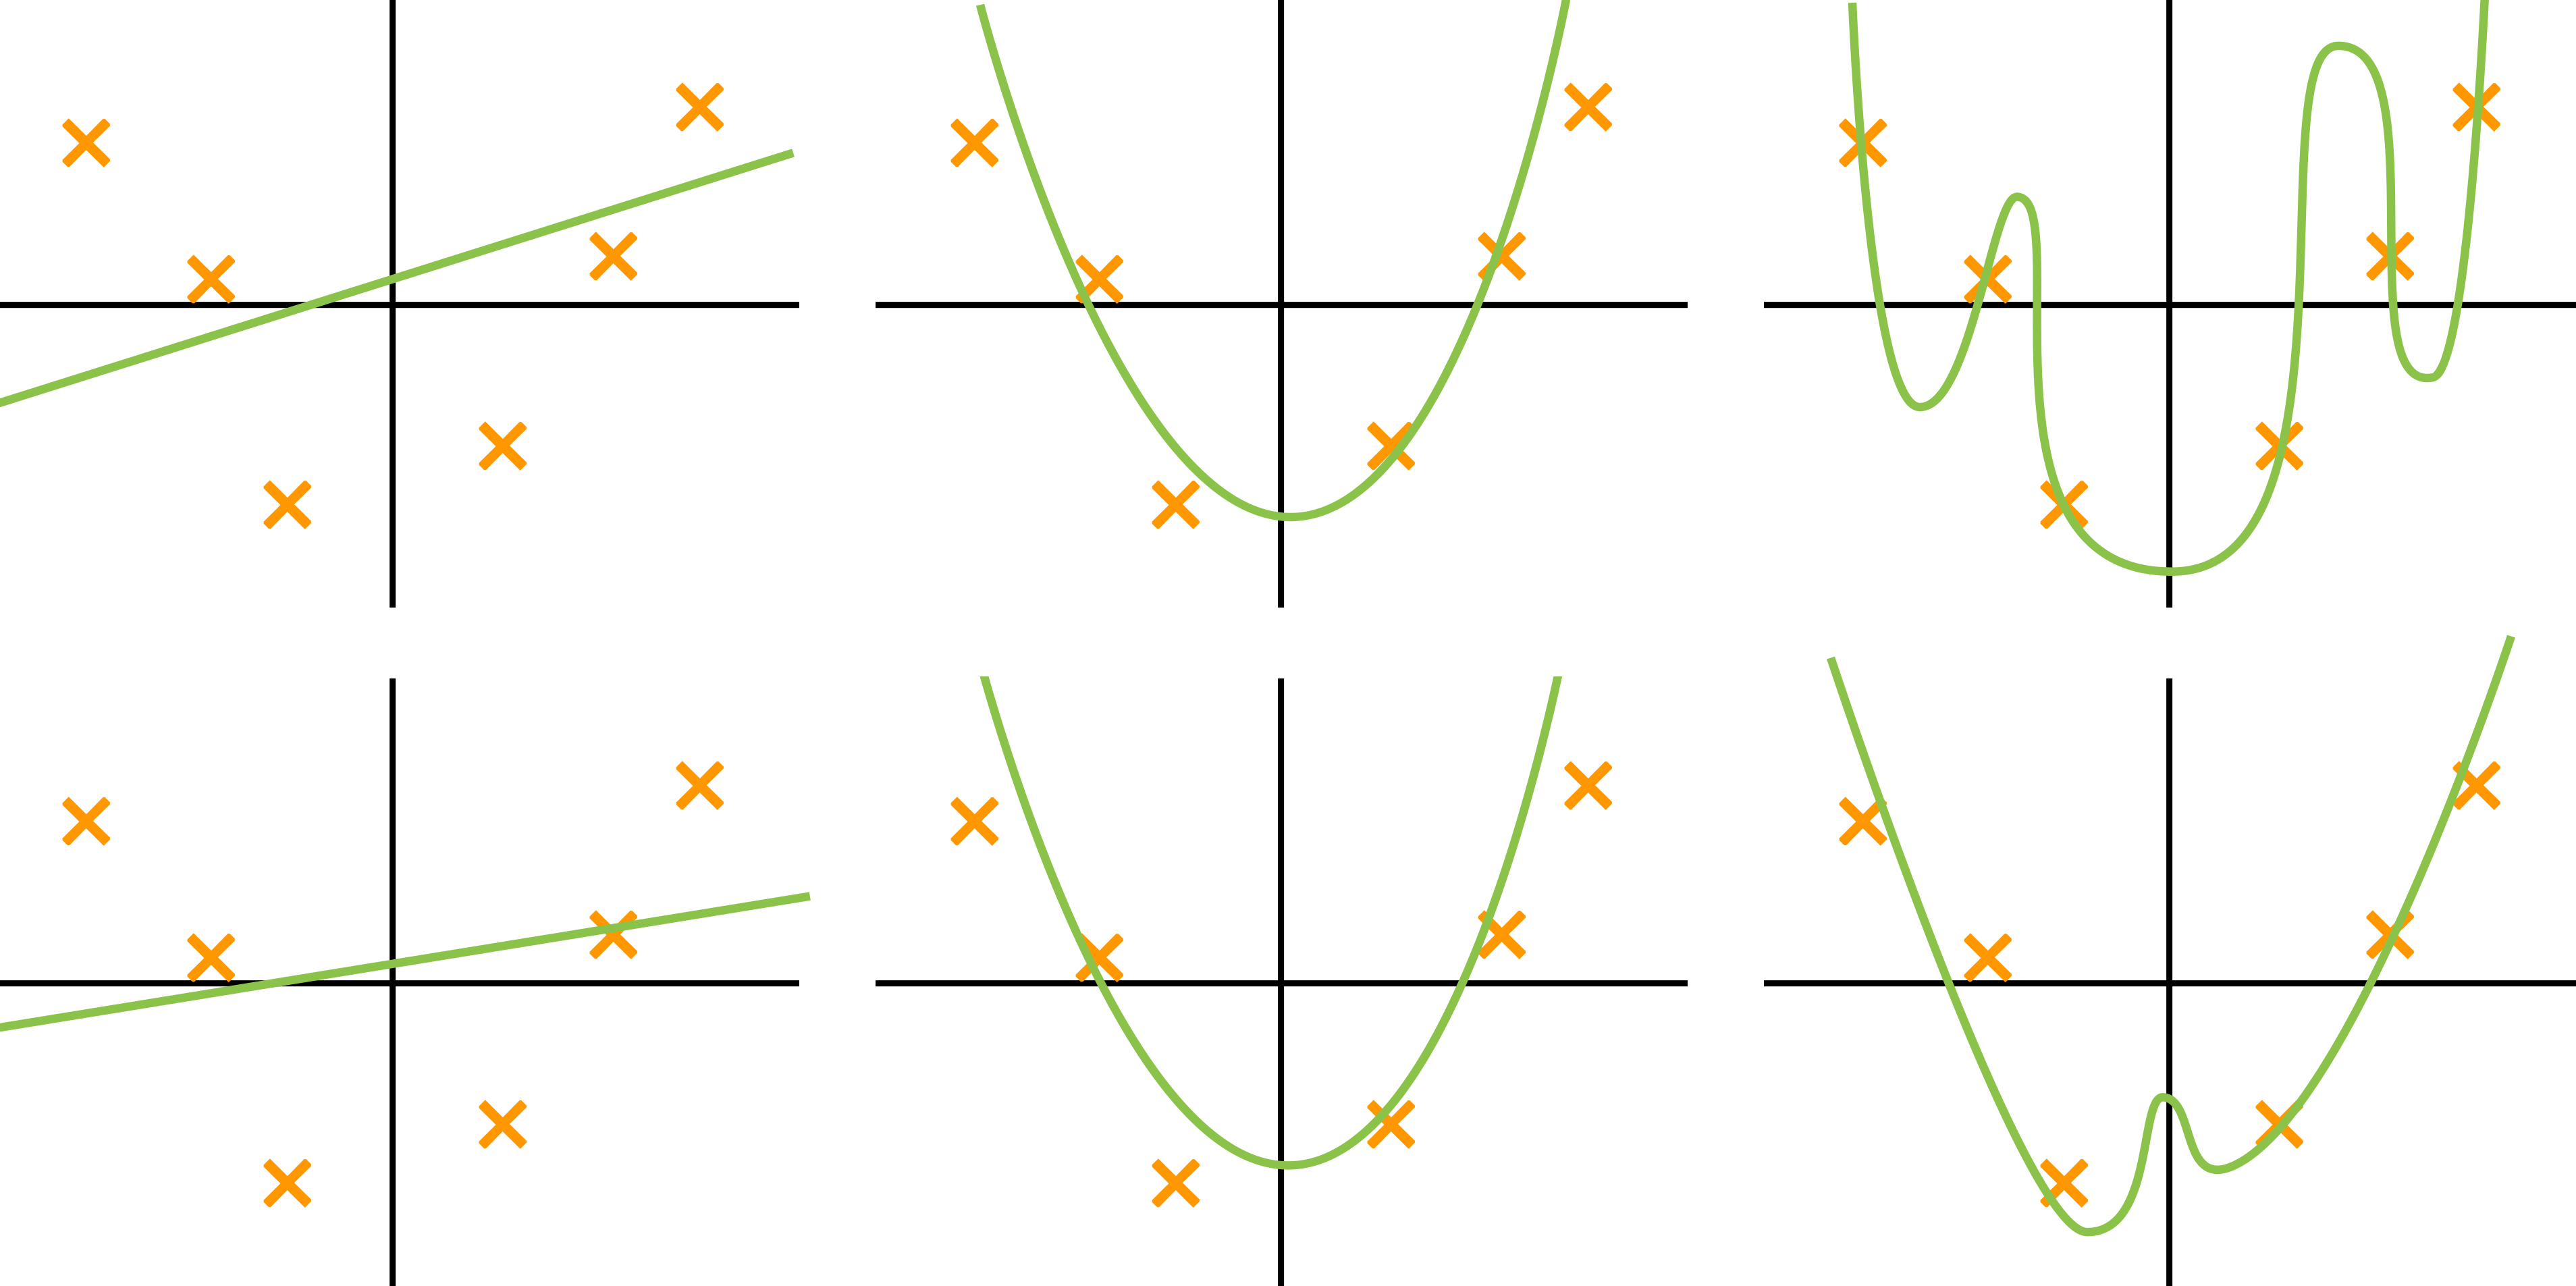
\includegraphics[width=\textwidth]{18.png}
\end{center}
Again, we see that $\lambda$ plays a similar role as $k$. It penalizes our interpolating polynomial $\beta^x$ from being too ``complicated''. What we're doing is trying to minimize the loss function, so $\lambda$ represents the ``balance'' between how much we want to minimize the sum of squares error and the regularization term.

On one end, $\lambda = 0$, and it's normal linear regression when we only care about minimizing the error. On the other end, as $\lambda \to \infty$, we only care about making the regularization term small, which pushes $\beta \to 0$. Reasonable values are somewhere in between, which try to strike a balance between the two errors.

\subsubsection*{Statistical learning theory}

We're on the edges of an idea: some sort of trade-off between simple and complicated, loose and tight. To pin down this idea mathematically, we're going to need to describe machine learning using some tools from probability, an approach that forms the basis of \textbf{statistical learning theory}.

The change is to move from considering data as something fixed and given to us, to something that's random, something that comes from a distribution. There's the set of \textit{all} possible examples, and the data we get is drawn from this set probabilistically, as specified by a \textbf{distribution}. We only run the learning algorithm on a \textbf{sample} of all of these possible examples.

The data itself might not be deterministic. Consider trying to learn a ``fuzzy'' boundary for a classification problem. The same point might not always be given to us as the same class. In this case, if you're far from the boundary, the probability that the sample we get is ``correctly'' classified goes higher. And the nearer you get, the more \textbf{noise} there is; the more likely our sample is to flip the other way and be ``incorrectly'' classified.

It's often the case in the real world that our examples are fuzzy; if you tried to predict whether a given animal is more likely to be a dog or a cat given its height and weight, you're going to have some inputs that map to different outputs. Here, are two distributions, one noisier than the other, and two samples drawn from each:

\vspace{0.5em}
\begin{center}
  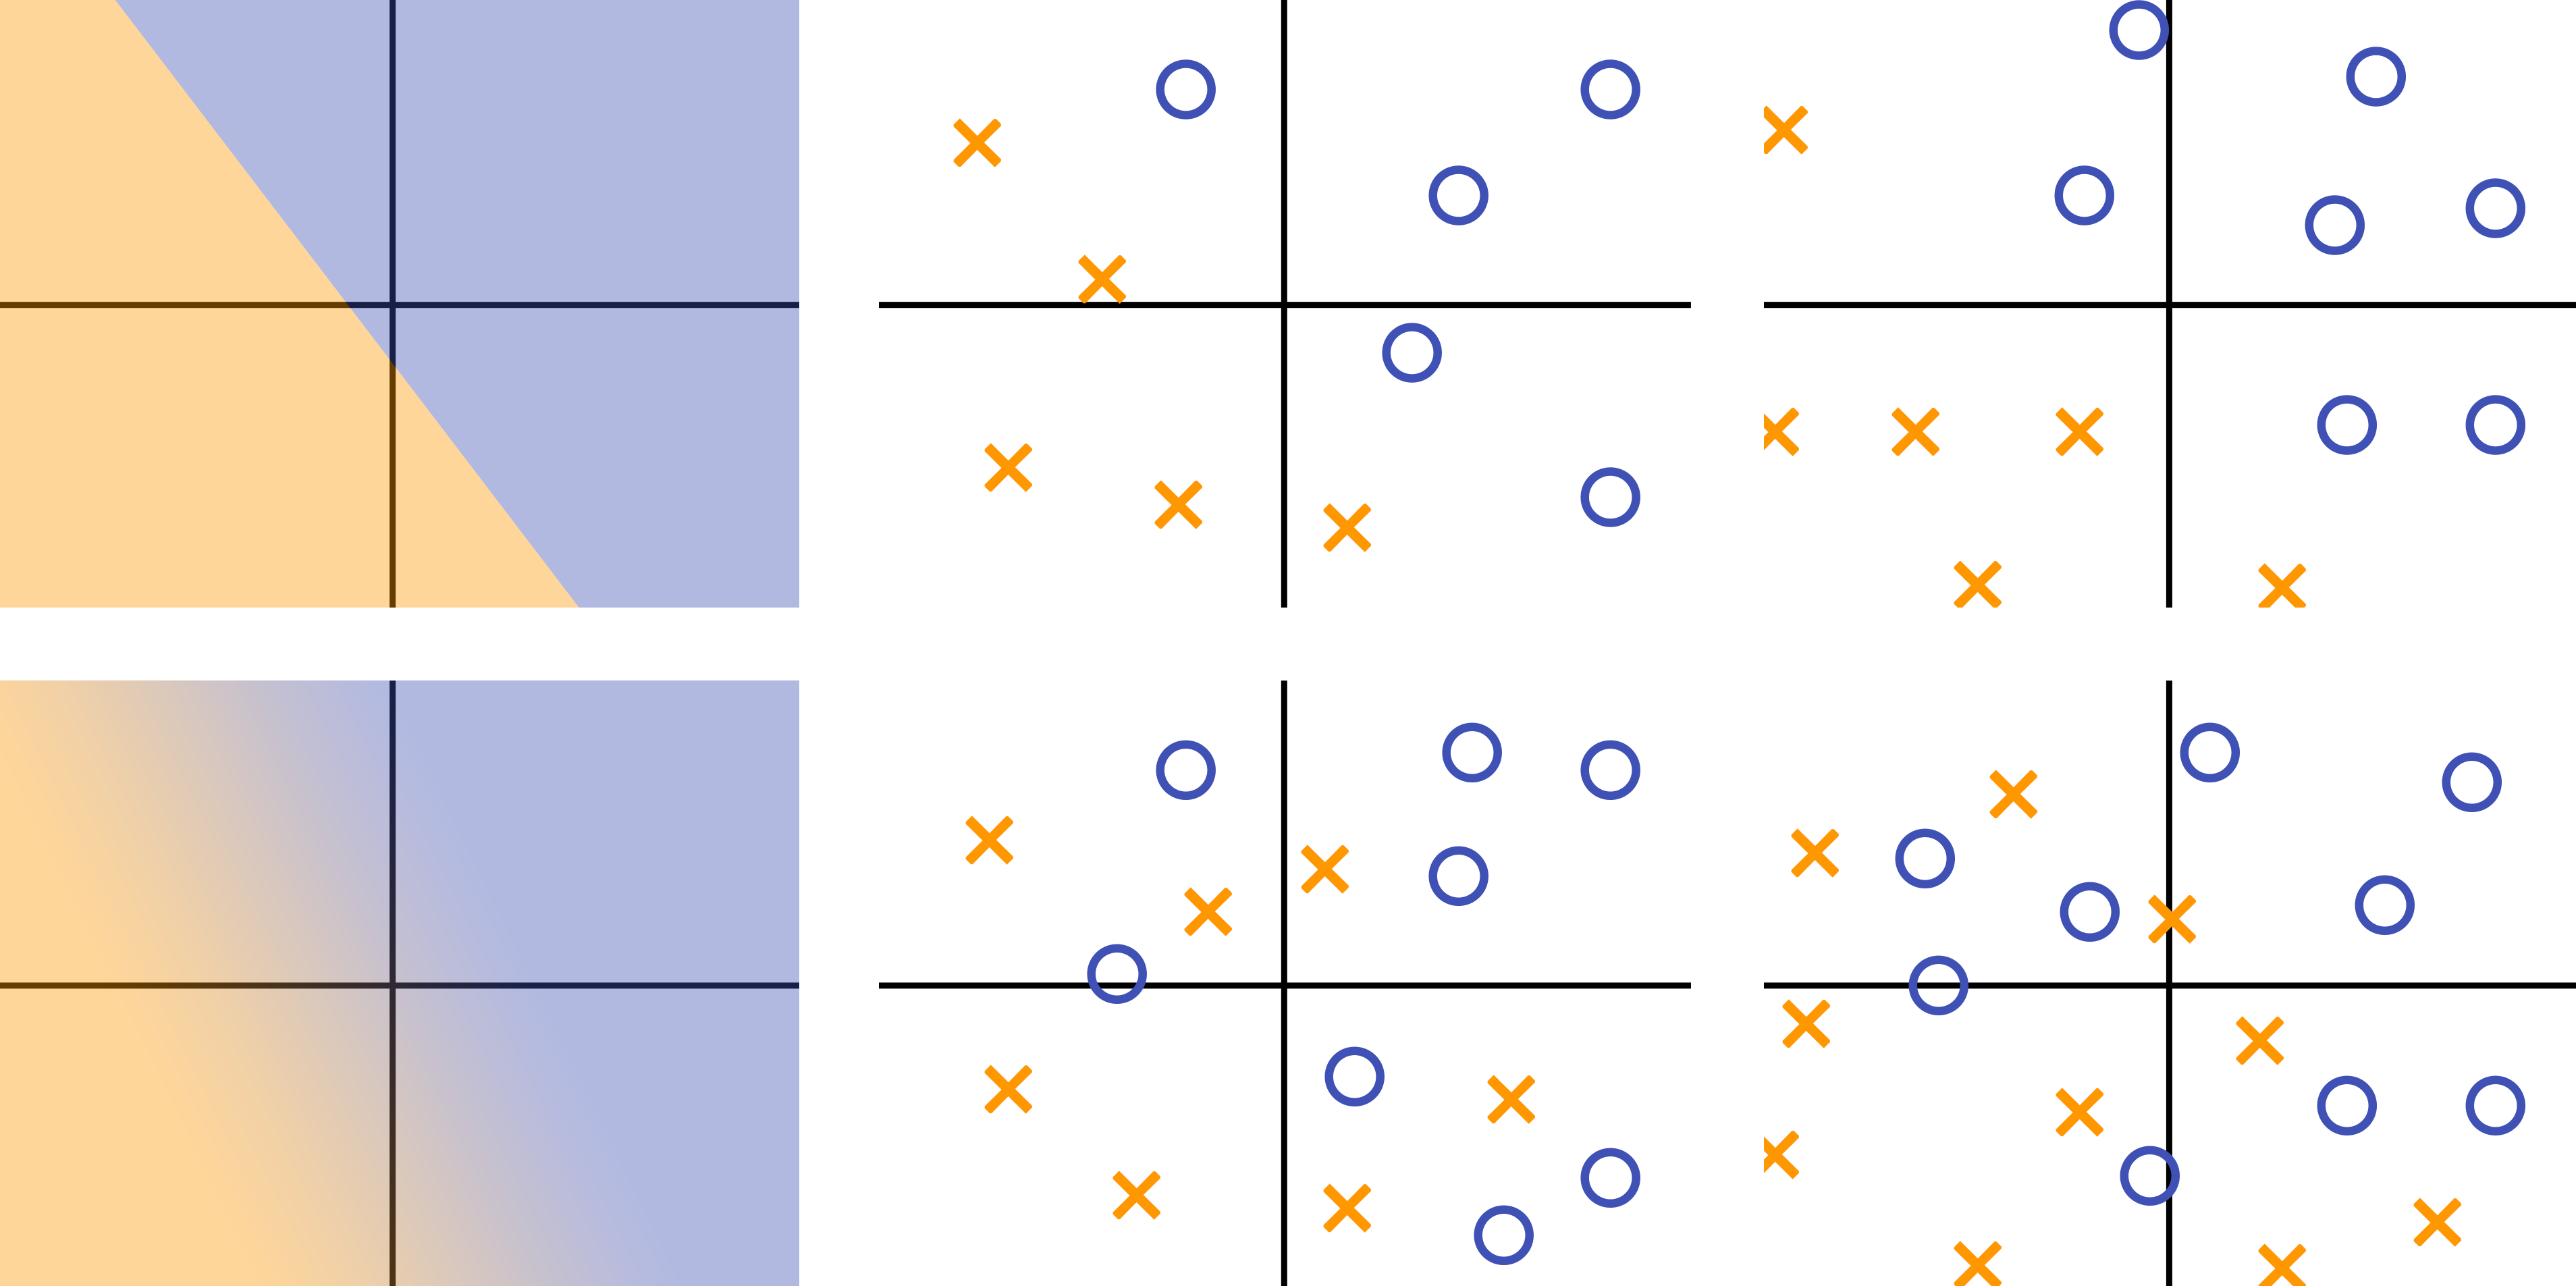
\includegraphics[width=\textwidth]{19.png}
\end{center}
\vspace{0.5em}

Let's restate the classification problem in this light. There's some input space $X$, which we usually take to be $d$-dimensional vectors. Then there's the output space $Y$; in the classification problem it's a discrete set of labels, but in a general regression problem it could be general real vectors too. The goal is to learn some probability distribution $D$ on the set $X \times Y$. One way to think about $D$ is as an example generator: every time we ask for a sample from $D$, it picks some $(x, y)$ according to the probability distribution, and hands it to us.

Then we assume we have a sample $S$, which consists of, say, $n$ examples $(x_1, y_1), \ldots$, $(x_n, y_n)$, drawn independently from $D$. We then feed $S$ into a learning algorithm, and out comes a model $f$. We can think of a learning algorithm as a way to choose some $f$ out of the hypothesis space $H$, the set of all possible hypotheses we're considering. This is pretty meta, so it's important to think through the difference:

\begin{exrboxed}
  Let $x$ be some vector in the input space $X$.
  \begin{enumerate}
    \item How do you interpret $y$, as a random variable, over the possible $(x, y)$ drawn from $D$?
    \item Think of $S$ itself as a random variable. Then the learning algorithm produces a model $f$, and as it depends on $S$, it's a random function. How do you interpret $f(x)$, as a random variable, over the possible samples $S$ drawn from $D$?
    \item Now let's say we have a \textit{fixed} $S$, which produces a \textit{fixed} model $f$. How do you interpret $f(x)$, as a random variable, over the possible ways to draw $x$ from $D$?
  \end{enumerate}
\end{exrboxed}

\subsubsection*{Bias--variance tradeoff}

We know how to judge a particular \textit{model} $f$. We just draw $(x, y)$ from $D$, and we know that $f$ is a good model if it's pretty likely that $f(x)$ is $y$. The probability that $f(x)$ is \textit{not} $y$ is called the \textbf{generalization error}: it's how bad $f$ performs on the actual distribution $D$.

The goal of a learning algorithm is to find $f$ with as low generalization error as possible, given only a limited sample $S$. But we can't compute generalization error: \textit{we don't know the actual distribution}!

We can try to settle with measures like the \textbf{empirical error}, which is the average error in the sample $S$, rather than the entire distribution $D$. But the problem is that empirical error isn't always a good measure of generalization error: a \textit{really} overfitted $f$ would have zero empirical error, but huge generalization error:

\begin{center}
  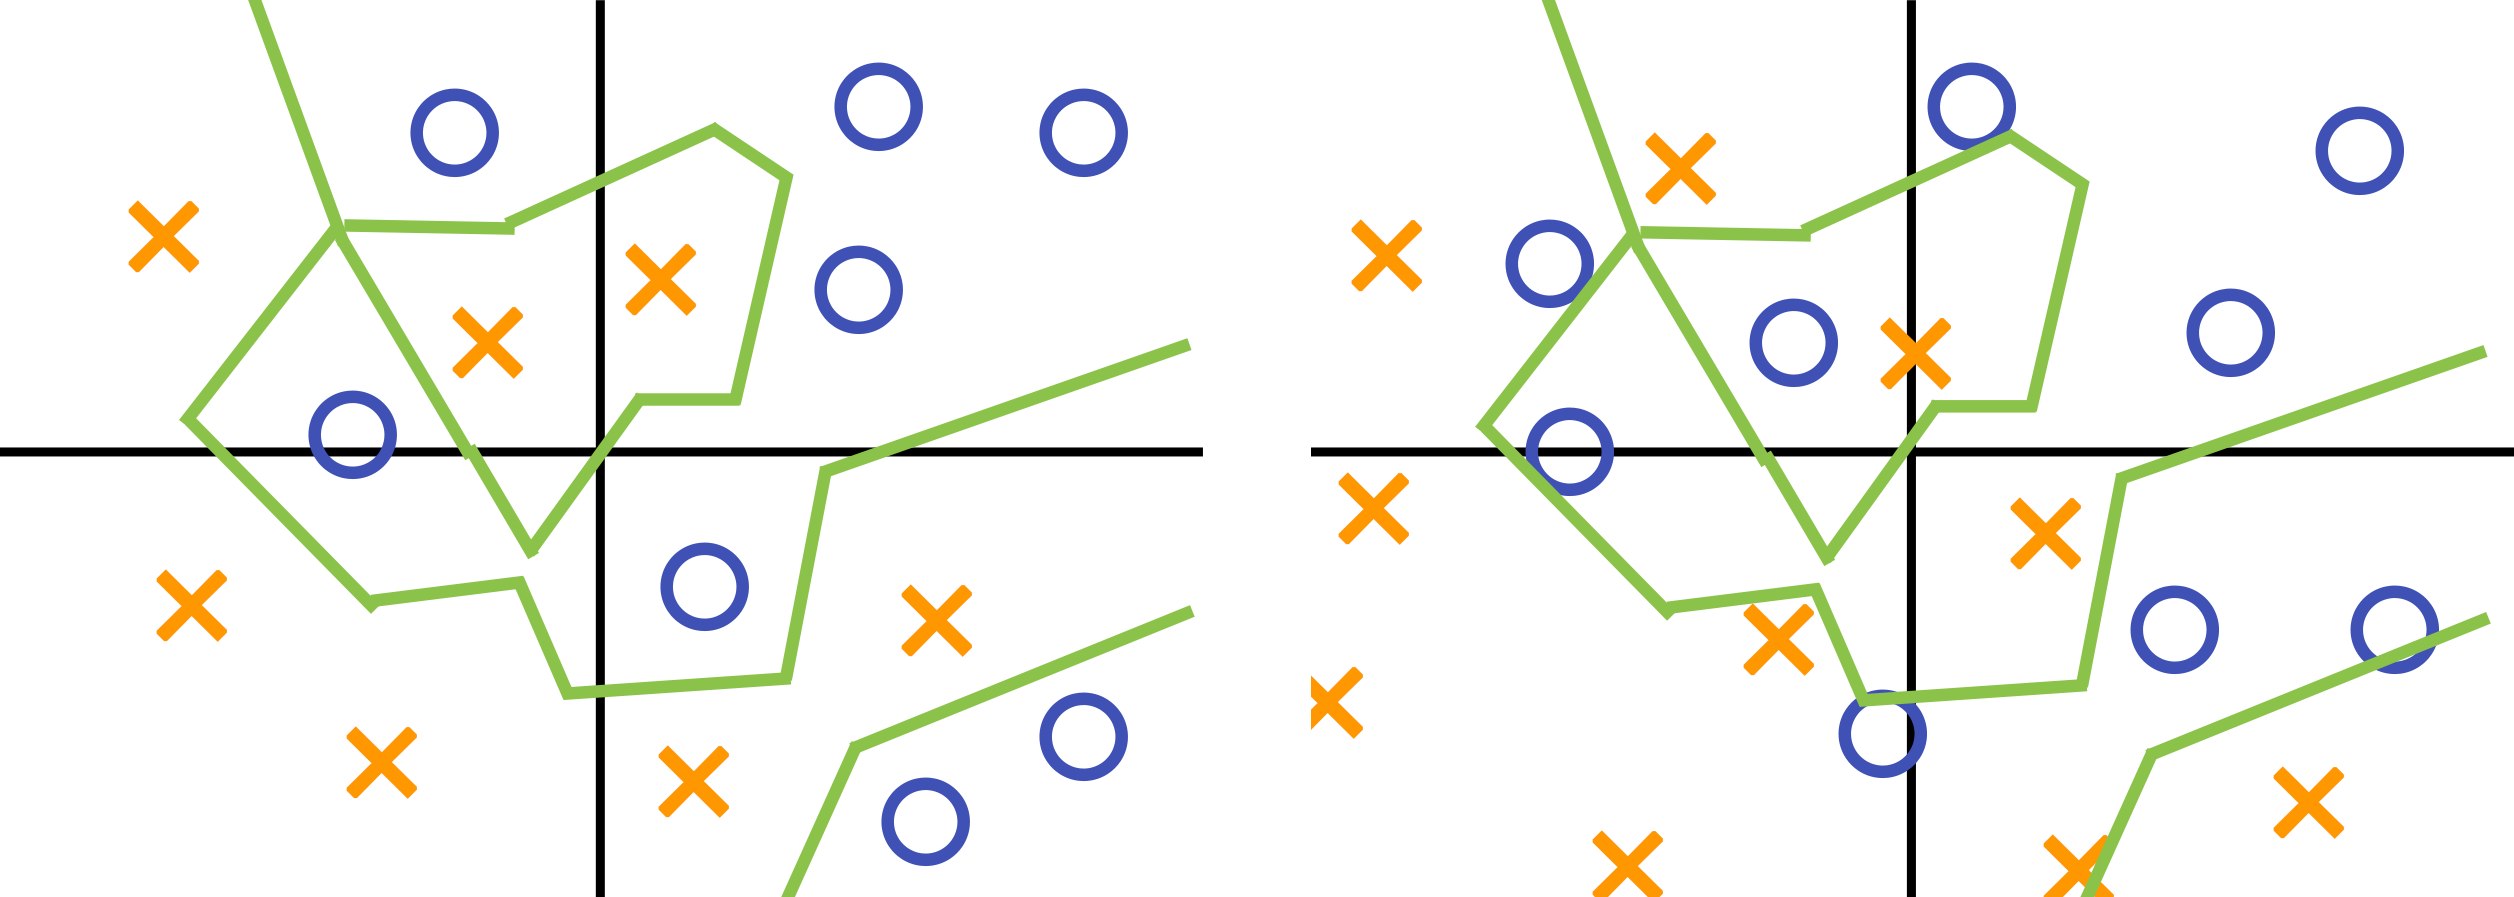
\includegraphics[width=0.66\textwidth]{20.png}
\end{center}

While overfitting is a property of a particular model, we can also describe learning algorithms that tend to produce overfitted models. If a learning algorithm was perfect, then it wouldn't matter what the sample we give it is; it'd always return the best possible model $f$. Unfortuantely, we have to settle for less. But if a learning algorithm is good, then we'd expect it to produce a similar model no matter what the sample we give to it.

Here's an example. The distribution $D$ represents a fuzzy classification boundary. Not only is the boundary fuzzy, but it's also more likely to draw samples from inside the boundary, rather than outside the boundary. The top row shows four samples from $D$. The second row represents the boundaries you'd get from running 1-nearest neighbors, and the third row represents what you'd get from running 20-nearest neighbors:

\begin{center}
  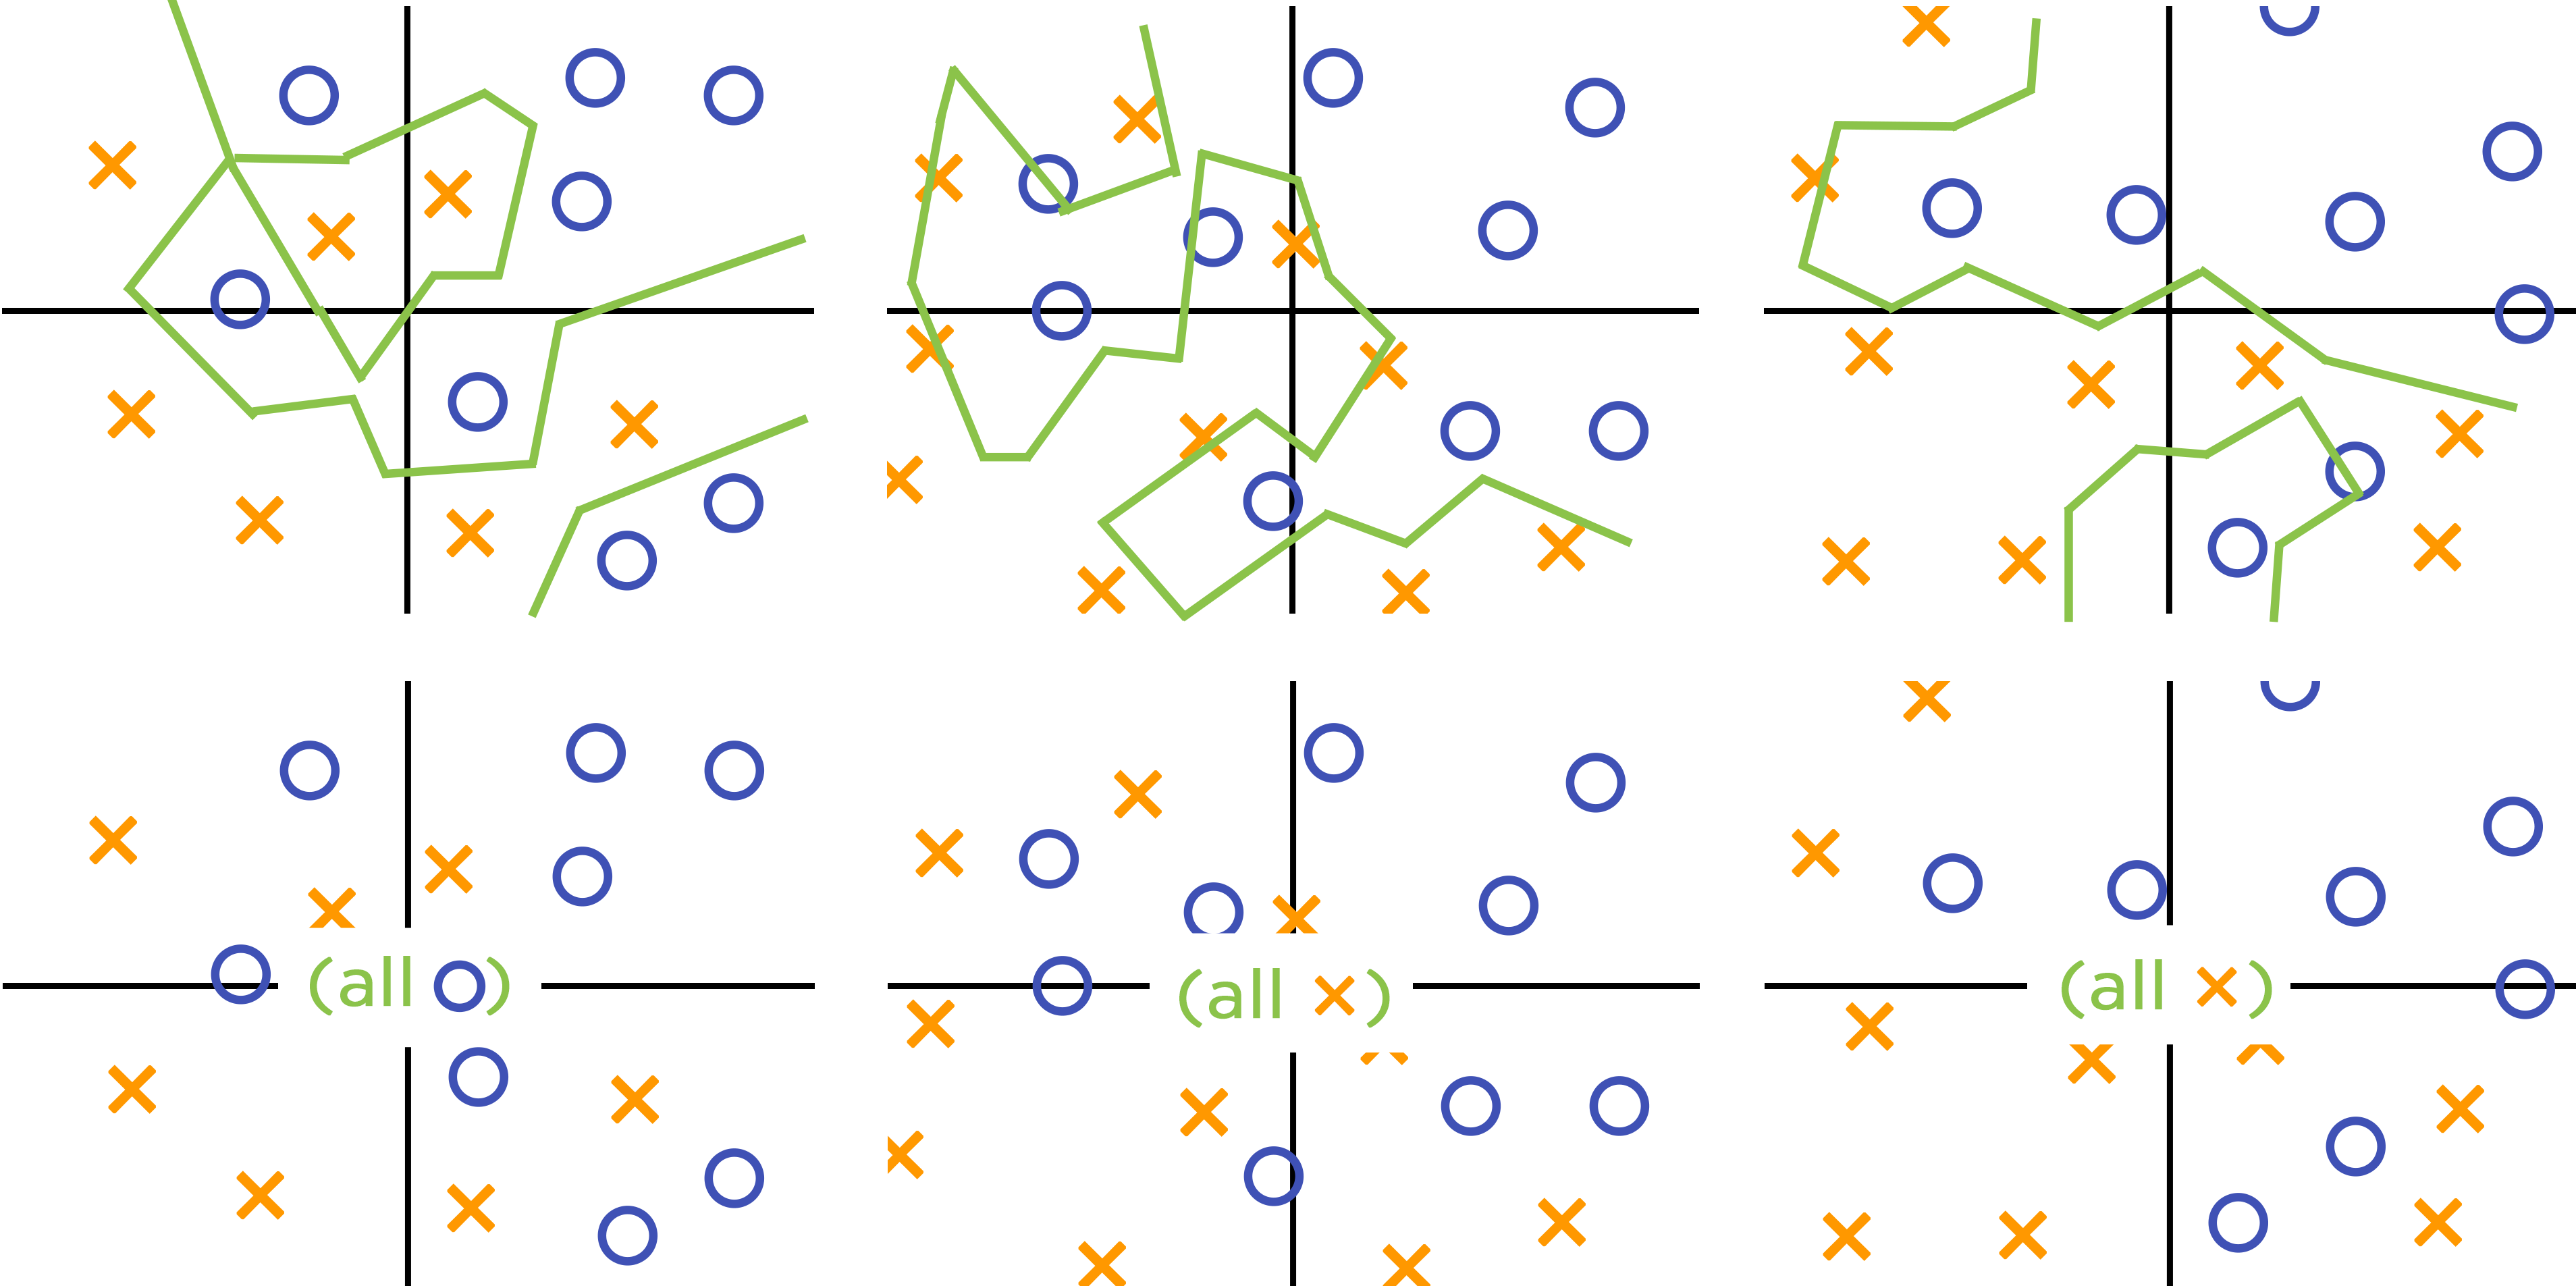
\includegraphics[width=\textwidth]{21.png}
\end{center}

We say a learning algorithm has high \textbf{variance} if the output varies a lot if you change the sample. We can measure this by looking at the variance of $f(x)$, over all $x \in X$, over all samples $S$. Here, 1-nearest neighbors has high variance, and we know a good learning algorithm cannot possibly have high variance. In contrast, 20-nearest neighbors produces similar boundaries each time; it's more likely to draw from inside the boundary, so even if you're far away from the boundary, most of the neighbors are more likely to be inside.

The way to describe how 20-nearest neighbors messes up is to say it has high \textbf{bias}. A learning algorithm has high bias if no matter what $f$ it chooses, it has high generalization error. It's high bias if it's not powerful enough to produce a good model in the first place. So note that 1-nearest neighbors has \textit{low} bias: it's \textit{possible}, although unlikely, for the algorithm to find really good decision boundaries.

Again, to clarify, bias and variance are a property of the \textit{learning algorithm}, and not the individual models they produce. Learning algorithms with high variance tend to produce models that are overfitted. Learning algorithms that have high bias tend to produce models that are underfitted.

This captures exactly what we've been seeing when we try to vary $k$ for $k$-nearest neighbors, or $\lambda$ for ridge regression. We're moving between the \textbf{bias--variance tradeoff}. Changing $k$ and $\lambda$ gives us different learning algorithms, moving from low-variance and high-bias, to high-variance and low-bias.

\subsubsection*{Cross-validation}

The way we choose hyperparameters, in practice, is through \textbf{cross-validation}. First, we split the data into training, validation, and test data. We pick some value of the hyperparameter, train it on the training set, then test how it performs on the validation set. We pick the hyperparameter according to what gives the best performance on the validation set.

Typically this is done through \textbf{early stopping}. Suppose, for example, that we were picking $\lambda$ for the polynomial regression we were doing earlier. The way early stopping would work is to start at some large value of $\lambda$, then keep decreasing $\lambda$. This, typically, decreases the empirical error on the validation set, up to a point. As soon as we hit that point---when decreasing $\lambda$ would make the error go up again---we stop. This is because the effect of $\lambda$ on the error is something like a U-shape:

\begin{center}
  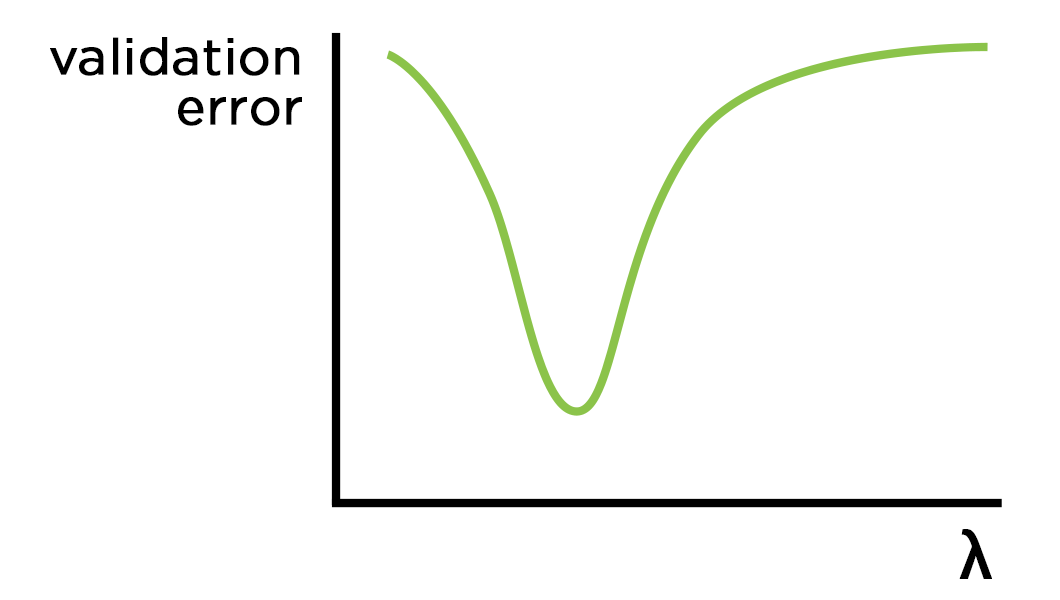
\includegraphics[height=1.8in]{22.png}
\end{center}

This U-shape makes sense intuitively. On the left side, you have low variance, but high bias, so we couldn't possibly find a good model in the first place. On the right side, you have high variance, but low bias, so you'd have to be really lucky to get a good model. This is a pretty common pattern in machine learning; the error is often a convex function of the parameters.

Some questions. Why do we have a test set? Well, the process of cross-validation can also overfit the data, so to get a good measure of the performance of the final model, we use the test data. This is why the test data is also called \textbf{holdout data}; it's data that's not used \textit{at all} in making the model or selecting the learning algorithm.

What if we want to make changes after seeing the final model's performance on the test set? Then you'd be liable to overfitting: improving performance on the test set \textit{specifically} is equivalent to just improving performance on the training and validation set. By not using the test set at all in the training process, it remains unbiased. Kind of like Goodhart's law, if you happen to know what that is.

What if we don't have enough data? This is a pretty common problem; often we don't have enough data to split it between three sets. One popular approach is to use \textbf{$n$-fold cross-validation}. Split the non-test data into $n$ sets, let's say $S_1, \ldots, S_n$. Fix a value for the hyperparameter. Then we can train on $S_2, \ldots, S_n$ and then validate on $S_1$, and we can also train on $S_1, S_3, \ldots, S_n$ and validate on $S_2$, and so on. We can then use the average validation error, and adjust the hyperparameter based on that.

How do we decide how to move the hyperparameter? In the case of, say, $n$-nearest neighbors, there are a discrete set of choices for $n$, and we can just check each one. But in the general case, the hyperparameters are real numbers, like $\lambda$. In this case, we can have some fixed \textbf{step size}, and we can decrease $\lambda$ by this step size each time.

But it turns out a better method is to use a learning rate, the heart of a method called gradient descent, which we'll talk about when we talk about neural networks. So keep this question in mind!

\subsubsection*{Model selection}

I know that was a lot of words, I'm sorry. Since this is supposedly a math camp, let's try to finish with some math. This is one of my favorite illulstrations of model selection, taken from MacKay's information theory book.

Let's say we have a sequence $S$, which is $-1, 3, 7, 11$. What are the next two numbers? Well, we can say $15, 19$, with the rule being $a_{n+1} = a_n + 4$. But what about $-19.9, 1043.9$, with the rule being $a_{n+1} = -\frac{1}{11}a_n^3 + \frac{9}{11}a_n^2 + \frac{23}{11}$? Both of these fit the data, yet one clearly ``feels better'' than the other.

We can write this out using Bayes's theorem. Let $H_1$ model the sequence as an arithmetic progression, and $H_2$ model the sequence as a cubic function of the previous term. We don't know the distribution of all possible ways $S$ could've been sampled. But to compare between $H_1$ and $H_2$, like we did in linear discriminant analysis, it suffices to just take the log ratio: \[
  \log \frac{P(H_1 \mid S)}{P(H_2 \mid S)}
  = \log \frac{P(H_1)}{P(H_2)} + \log \frac{P(S \mid H_1)}{P(S \mid H_2)}.
\]
We can say that $H_1$ is more likely just beacuse arithmetic progressions are more common than cubic recursions, or in other words, $P(H_1) > P(H_2)$. But let's not make that assumption, and concentrate on the difference between $P(S \mid H_1)$ and $P(S \mid H_2)$.

To find $P(S \mid H_1)$, we need to say exactly how $H_1$ generates sequences. There are two parameters of an arithmetic progression: the first term and the common difference. Suppose that these were both integers chosen uniformly from $-50$ to $50$, because we have to make \textit{some} assumptions. There's only one possible choice of first term and common sequence that could give rise to $S$, which gives
\[
  \log P(S \mid H_1) = \log \left(\frac{1}{101} \cdot \frac{1}{101}\right) = -9.23.
\]
Let's make similar assumptions to compute $P(S \mid H_2)$. It's specified by the first term, and then each of the coefficients in $ax^3 + bx + cx + d$. We'll assume that $a$, $b$, $c$, and $d$ are fractions, with denominators between $1$ and $50$, and let's say their numerators are from $-50$ to $50$, like the first term. There's essentially only one way to choose the coefficients, but we have to account for equal fractions. Doing this, we get
\[
  \log P(S \mid H_2) = \log \left(\frac{1}{101} \cdot \frac{4}{101} \cdot \frac{1}{50} \cdot \frac{4}{101} \cdot \frac{1}{50} \cdot \frac{1}{101} \cdot \frac{50}{50} \cdot \frac{2}{101} \cdot \frac{1}{50}\right)
  = -31.35.
\]
That's a \textit{huge} difference. Of course, the specific probabilities will depend on how we assume $H_1$ and $H_2$ generate their hypotheses, but the general idea is there. As $H_2$ has more parameters, the probability we select any specific choice of parameters is smaller than $H_1$. So Bayes's theorem leads to Occam's razor.

This fits into our discussion of bias and variance earlier. In this case, $H_1$ and $H_2$ have the same ``bias'', since they both fit the sample equally well. It's just the case that $H_1$ is ``lower variance'' than $H_2$. The situation would be different if $H_2$ could fit the data but $H_1$ couldn't.

\clearpage

\section{Neural networks (August 8)}

\textit{Prerequisites:} Matrices, vectors, differentiation, the first seminar. Nice, but not necessary: matrix differentiation, the second and third seminars.

\subsubsection*{Gradient descent}

Time to tie up some loose ends. We've talked about gradient descent in each of the past three seminars and it's time to finally talk about what it is. Note that each time we cited gradient descent was an optimization problem. What's the $\beta$ that minimizes this loss function? What's the $k$ or $\lambda$ that minimizes validation error?

Generally, each of these problems have the same form: minimize some objective function $f$ on the input $x$. When the gradient $\nabla f$ is easy to compute, and even in some cases when it isn't, we can use \textbf{gradient descent} to look for a minimizer $x$.

Consider, first, the case when $f$ is a one-dimensional function. We know that $f'(x)$ represents the slope of the tangent line; it points toward the direction where $f(x)$ grows the fastest, locally. In multiple dimensions, it's the same idea with $\nabla f(x)$.

\begin{center}
  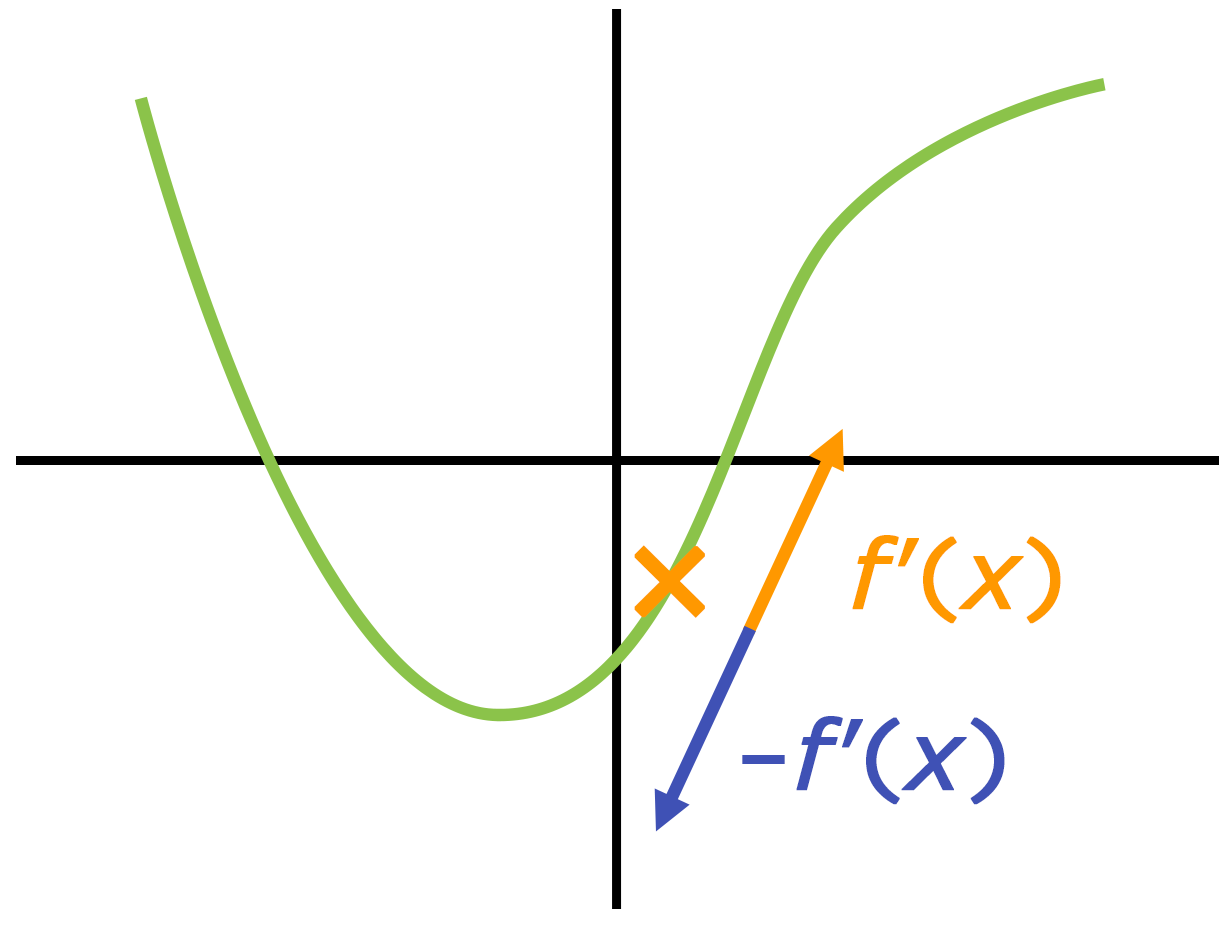
\includegraphics[height=1.5in]{23.png}
\end{center}

So if we want to make $f(x)$ small, we should move $x$ \textit{against} the direction of the gradient. Assume we have some hyperparameter $\alpha$, the \textbf{learning rate}. Set $x$ to be something arbitrary. Then in each step, we change $x$ to be $x - \alpha \nabla f(x)$, and repeat until we're happy with how small $f$ is. We can stop after a fixed number of steps, or when the change in $x$ is small enough, or when $\nabla f(x)$ has small enough norm. Note that gradient descent doesn't require us to compute $f(x)$ anywhere in the process; we only need to do $\nabla f(x)$ fast.

There are lots of questions about this. We won't go through them in much detail, but we will outline the answers. First, how do we pick $\alpha$? In the convex case, there's always some $\alpha$ such that gradient descent converges, and anything smaller than that $\alpha$ would converge too. The idea is that larger values of $\alpha$ can continually ``overshoot'' and never hit the minimum. But if $\alpha$ is too small, then convergence would take a really long time.

\begin{center}
  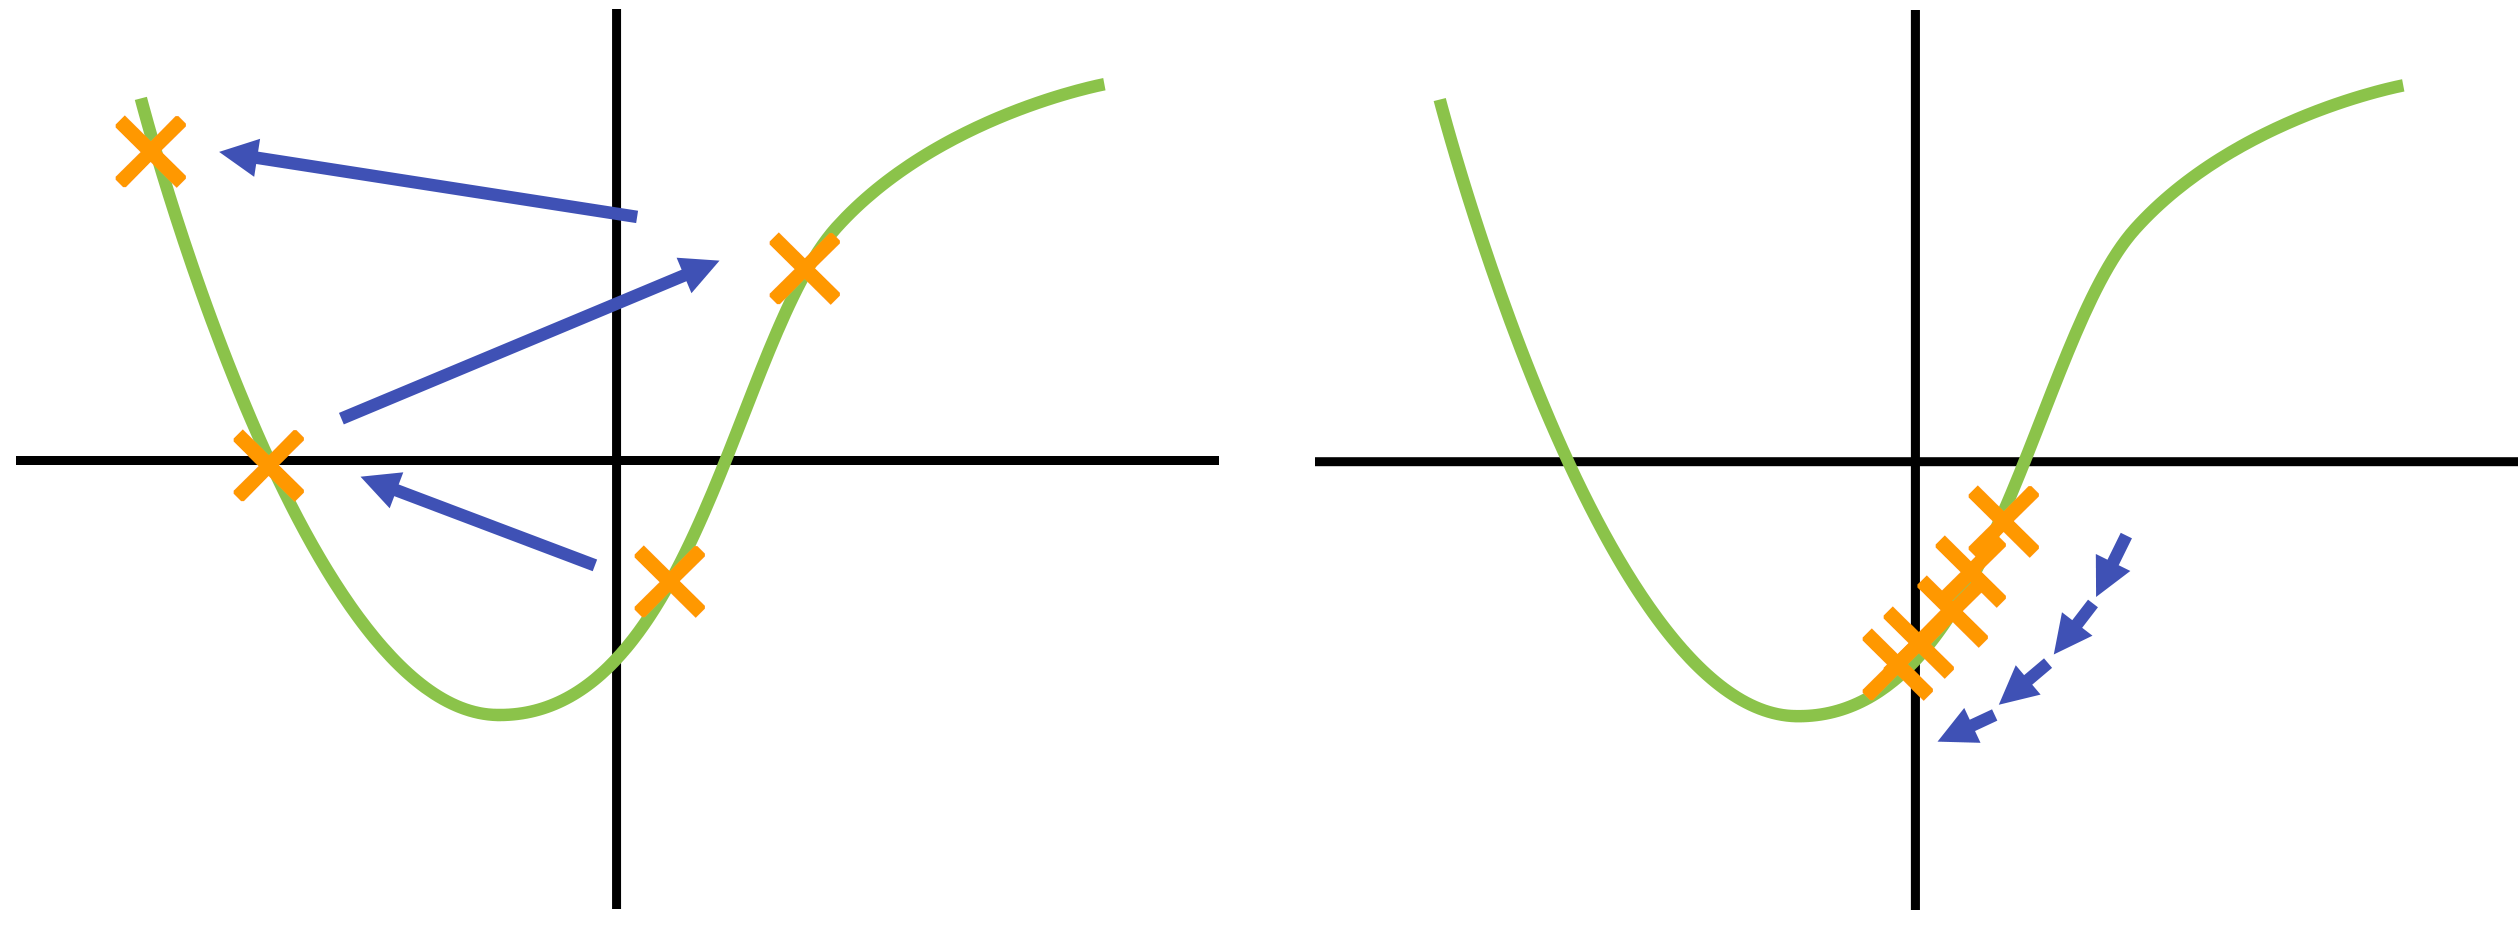
\includegraphics[height=1.5in]{24.png}
\end{center}

So typically, you'd want some sort of \textbf{adaptive step size}, where the size of $\alpha$ \textit{also} depends on the value of $\nabla f(x)$. Popular implementations of this are \textbf{AdaGrad} and \textbf{Adam}. Alternatively, you could add something called \textbf{momentum}, where instead of $\nabla f(x)$, the update is a combination of $\nabla f(x)$ and the previous direction of the update.

Then how about gradient descent when $\nabla f(x)$ is difficult to compute analytically? Typically, you can use tricks like \textbf{numerical differentiation} or \textbf{automatic differentiation} to compute these derivatives. What about if you know it analytically, but it's just expensive to compute? For example, for ridge regression on $\beta$ on the points $(x_1, y_1), \ldots, (x_n, y_n)$, the gradient of the loss is
\[
  \nabla L(\beta) = -\sum_{i=1}^n 2\left(y_i - \beta^Tx_i\right)x_i + 2\lambda\beta.
\]
The sum can have thousands of terms when $n$ is large, and you're also working with hundred-dimensional vectors! In this case, you can do \textbf{stochastic gradient descent}, which appears so often that it's called SGD. Instead of computing the whole gradient, you just compute it for a randomly chosen term in the sum. In practice, the contributions of each term will average out. Regular gradient descent is sometimes called \textbf{batch gradient descent}, or BGD, in contrast.

Finally, how about gradient descent on non-convex functions? That's an entire can of worms that I really don't have the time to talk about, so I'll leave this one for you to read more about.

\subsubsection*{Neural networks}

Recall that when we try to do a linear regression, we want to fit a series of inputs and outputs $(x_1, y_1), \ldots, (x_n, y_n)$. And we assume that each $x$ is a $d$-dimensional vector, and each $y$ is a $k$-dimensional vector. Then the fit $\beta$ would be a $d \times k$ matrix, and there'd be a constant $k$-dimensional vector $\beta_0$, and we try to fit $\beta^Tx_i + \beta_0$ to match $y_i$.

Well, training a \textbf{layer of neurons} is like a spicy linear regression. A layer of neurons takes some $d$-dimensional vector $x$, and multiplies it with the \textbf{weights} $W$, a $d \times k$ matrix. There's also the \textbf{bias weights} $W_0$, a $k$-dimensional vector. The resulting $k$-dimensional vector, $W^Tx + W_0$, is known as the \textbf{pre-activation}, which we call $z$. So far it's the same, except we call $\beta$ and $\beta_0$ as $W$ and $W_0$ instead.

The new part comes with some scalar function $f$, called the \textbf{activation function}. We $f$ to each coordinate of $W^Tx + W_0$ to get $f(W^Tx + W_0)$, the $k$-dimensional vector that the layer outputs. This is called the \textbf{activation} of the layer, which we call $a$. Hence a neuron is represented with its weights $W, W_0$, and its activation function $f$:

\begin{center}
  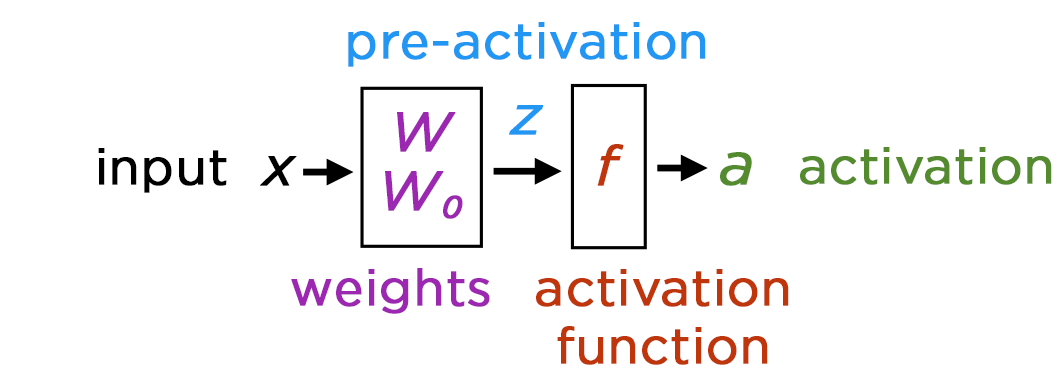
\includegraphics[height=1.4in]{25.png}
\end{center}

Now let's talk about finding weights. We want to find them such that each $a_i = f(W^Tx_i + W_0)$ matches $y_i$. Usually we have some loss function $L$, and we minimize the sum of $L(a_i, y_i)$. Note that linear regression is a special case of a neural network: for a linear regression, the activation is $f(x) = x$, and the loss is $(y_i - a_i)^2$.

% Unlike linear regression, when we try to find the $W$ for a layer of neurons, the choice of $f$ and $L$ mean we \textit{can't} find an analytical solution. Hence, we instead use SGD. After all, it's an optimization problem: minimize the loss give the parameters $W$.

And that's it. We've just described a single-layer neural network, which is nothing more than a linear transformation of the input, fed through an activation function. If it sounds simple, you're right; a single layer is pretty simple in itself.

What makes it a neural network, though, is through stacking several layers together. More layers means the network has more \textbf{depth}, and it's where we get the name \textit{deep} learning. If the $i$th layer had weights $W_i, W_{i, 0}$, and activation function $f_i$, then we'd represent it with this diagram:

\begin{center}
  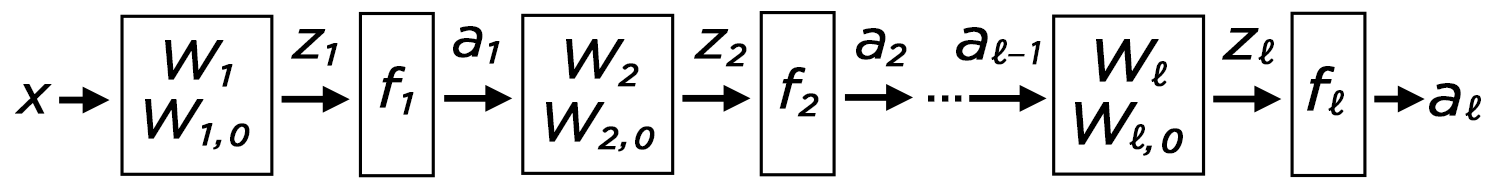
\includegraphics[width=\textwidth]{26.png}
\end{center}

In essence, that's all a neural network is. A linear transformation, followed by an activation function, and so on. To be technical, we described a specific kind of neural network called a \textbf{multilayer perceptron}, but when people say ``neural network'' without qualification, they usually refer to this.

\subsubsection*{In context}

Let's take a step back, and look at the neural network in context. So far, what we've described is a \textit{model}. A neural network is a model: it takes inputs, and gives outputs. It is not a \textit{learning algorithm}, not in itself. To specify the learning algorithm, we need to talk about how, given the input, we produce a model.

Generally, this process is called \textbf{training}. We \textit{train} a given neural network to match training data by adjusting its weights. Often, the choices of $f$ are complicated enough that we can't find the weights analytically, so instead we do something called backpropagation. The idea is to apply gradient descent on each layer of the network; we'll talk about this more later.

But this isn't \textit{quite} a learning algorithm. In order to train a neural network, you need to specify what the network looks like in the first place. How many layers does it have, what are their sizes, what's the activation function? These are all called the \textbf{architecture} of the network. So the whole learning algorithm is something like this:

\begin{center}
  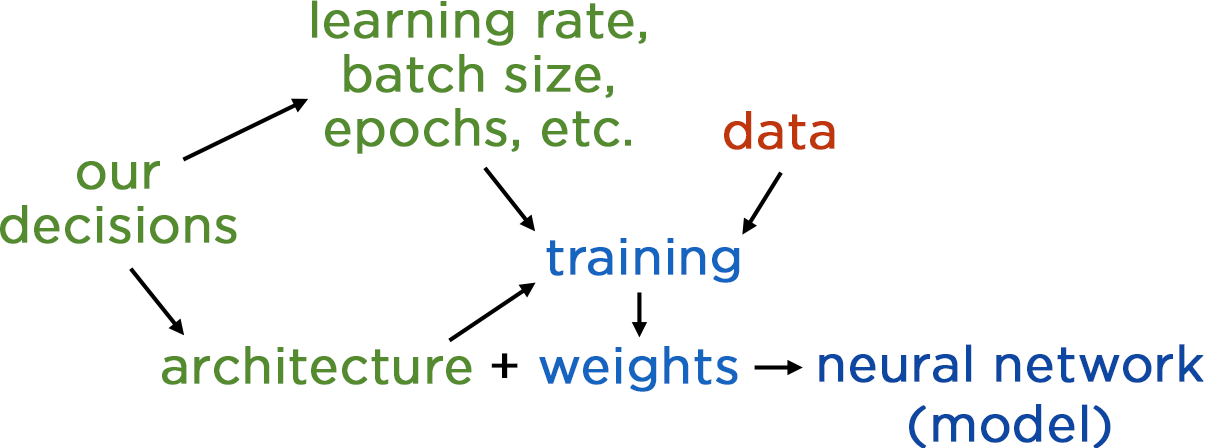
\includegraphics[height=1.5in]{27.png}
\end{center}

And the thing about this whole learning algorithm is that there are \textit{lots} of hyperparameters. The architecture of the network is a hyperparameter. And training takes a lot of hyperparameters, like learning rate, and even more if you choose to use adaptive step size or momentum.

With all of these hyperparameters that go into using neural networks, choosing them is sometimes more \textit{art} than science. As we talked about in the generalization seminar, more parameters means the model can fit all sorts of underlying patterns. But it's \textit{precisely} because of this we risk overfitting. In fact, networks can approximate \textit{any} function arbitrarily well, a result of \textbf{universal approximation theorems}. So choosing architecture and training the network needs a lot of care.

We'll spend the rest of the time talking about how backpropagation works, exactly, how architecture is designed, and how training is done in practice.

\subsubsection*{Backpropagation}

The way we want to train a neural network, in principle, is to do some sort of gradient descent on the weights. The key thing we need to be able to do is compute the gradient of the loss, $L$ with respect to the weights, $W$; this is the only thing we need to do gradient descent.

The way we compute this gradient is \textbf{backpropagation}, which is a fancy word for ``using the chain rule multiple times''. Let's consider a single layer, with input $x$, weights $W, W_0$, and activation function $f$. Recall that the pre-activation is $z = W^Tx + W_0$, and the activation is $a = f(z)$.

From the chain rule, we know that \[
  \frac{\partial L}{\partial W} = \frac{\partial L}{\partial a} \cdot \frac{\partial a}{\partial z} \cdot \frac{\partial z}{\partial W} = \frac{\partial L}{\partial a} \cdot \frac{\partial a}{\partial z} \cdot x^T.
\]
We get $\frac{\partial L}{\partial a}$ from the actual loss function, and $\frac{\partial a}{\partial z}$ from the choice of $f$.

Now let's consider this for $\ell$ layers. Let the $i$th layer have weights $W_i, W_{i, 0}$ and activation function $f_i$. Note the activation of the $i$th layer, $a_i$, is the input to the $i+1$st layer. The input to the entire network is $x = a_0$, and the output is $a_\ell$.

\begin{center}
  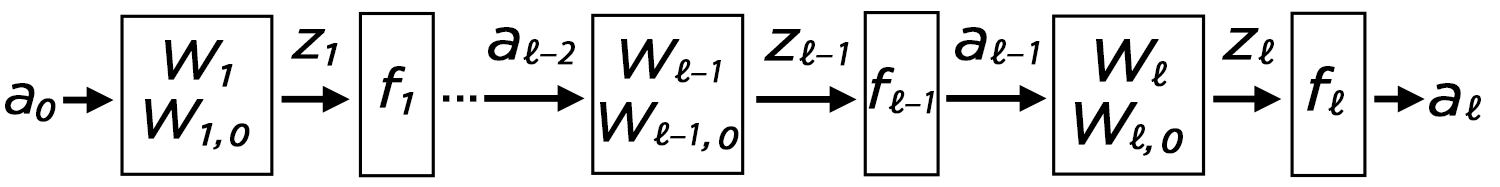
\includegraphics[width=\textwidth]{28.png}
\end{center}

Now for the last layer, as above, \[
  \frac{\partial L}{\partial W_\ell} = \frac{\partial L}{\partial a_\ell} \cdot \frac{\partial a_\ell}{\partial z_\ell} \cdot a_{\ell - 1}^T.
\]
So that tells us how to compute the gradient for the last layer. For the layer behind it:
\begin{align*}
\frac{\partial L}{\partial W_{\ell - 1}}
&= \frac{\partial L}{\partial a_\ell} \cdot \frac{\partial a_\ell}{\partial z_\ell} \cdot \frac{\partial z_\ell}{\partial a_{\ell - 1}} \cdot \frac{\partial a_{\ell - 1}}{\partial z_{\ell - 1}} \cdot \frac{\partial z_{\ell - 1}}{W_{\ell - 1}} \\
&= \frac{\partial L}{\partial a_\ell} \cdot \frac{\partial a_\ell}{\partial z_\ell} \cdot W_\ell^T \cdot \frac{\partial a_{\ell - 1}}{\partial z_{\ell - 1}} \cdot a_{\ell - 2}^T.
\end{align*}
And you can keep going. We don't have to recompute every term of this product, since we've already computed most of them for the layer in front. This produces something like this diagram:

We won't burden ourselves with the implementation, as this is a \textit{math} camp, but this should at least show that doing the update step scales linearly in terms of the number of layers. So as long as you know how to differentiate fast-ish and multiply matrices fast-ish, backpropagating is fast-ish.

It bears repeating: what we've done is said \textit{how} to do the update step of gradient descent. We still haven't talked about the specifics of \textit{when} we do this update step in the first place; we'll talk about this when we get to training.

\subsubsection*{Architecture}

In practice, how is architecture designed? First, we'd need to specify the number of layers, which describes the \textbf{network depth}. For most practical purposes, there are at least two layers. The last layer is called the \textbf{output layer}, and the intermediate layers are called \textbf{hidden layers}. When people say ``single-layer neural network'' they often mean one hidden layer, and one output layer.

\begin{center}
  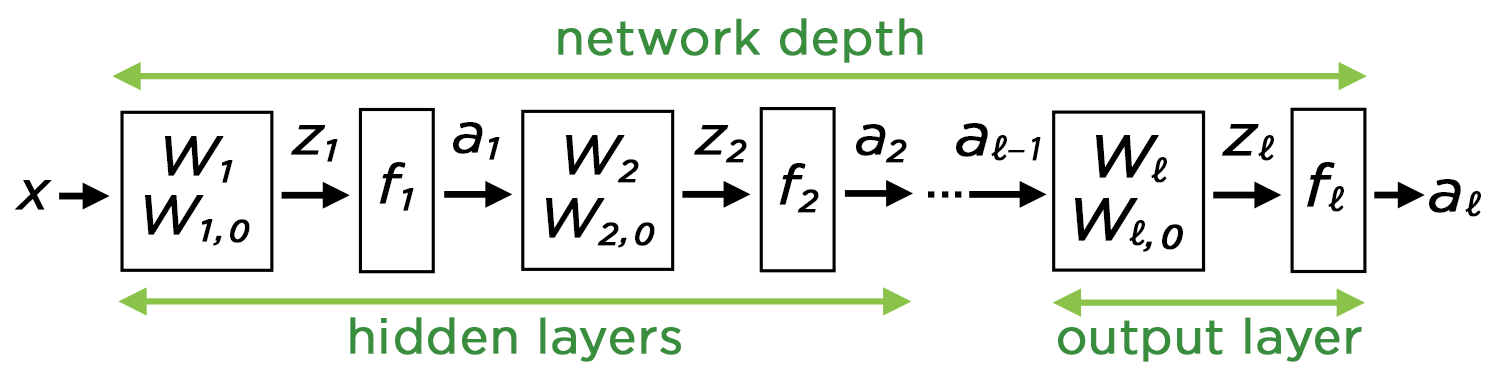
\includegraphics[width=\textwidth]{29.png}
\end{center}

Then you need to describe each layer, which means describing two things: its activation function, and its \textbf{width}. The width is the dimension of the output vector, also called its number of \textbf{units} or \textbf{nodes} or \textbf{neurons}. We haven't talked about the choice of activation function, which is a crucial part of what makes it a neural network. If all activation functions were the identity, then the entire network would just be a linear transformation!

There are only a handful of widely-used activation functions. We think of choosing activation functions for hidden layers and output layers separately, and we usually pick the same activation function for each of the hidden layers in a network. For the first part, let's talk about hidden layer activations.

One that used to be popular is the \textbf{sigmoid function}\[
  \sigma(x) = \frac{1}{1 + e^{-x}}.
\]
I'm not sure why it was popular, other than the fact it has a simple derivative, $\sigma(x) = \sigma(x)\left(1 - \sigma(x)\right)$, and it's non-linear. The problem with sigmoid is that the gradients towards the tails become small \textit{really} fast, a problem known as \textbf{vanishing gradients}, which is a problem if you have a lot of layers.

The sigmoid is related to using $\tanh(x)$, which is a scaled and shifted sigmoid. One reason to prefer $\tanh$ is that it has stronger gradients, but it's also subject to the vanishing gradient problem. It still performs well, sometimes. Hence kernel SVMs that used $\tanh$ were popular shortly after neural networks first became popular.

The most popular activation function is probably the \textbf{rectified linear unit}, or ReLU, and its variants. It's simply \[
  \text{ReLU}(x) = \begin{cases}
  0 & \text{if } x < 0 \\
  x & \text{if } x \ge 0.
  \end{cases}
\]
As ReLU doesn't have a saturated gradient, it apparently tends to converge faster than sigmoid and its variants. It also isn't subject to vanishing gradients as much. In practice, a lot of ReLU variants avoid the flat $0$ for negative $x$, like \textbf{leaky ReLU} which is $0.01x$ for negative $x$, or \textbf{ELUs} or \textbf{GELUs} or \textbf{SELUs} or \textbf{Swish} or \textbf{Softplus}. Choosing between these is an art.

Choosing output activations is comparably much simpler. For regressions, we usually just have the identity for the activation. A common exception is when we want the output to be a probability, which also comes up when we do classification with only two classes. In that case, we use $\sigma(x)$.

Note that it lies in the range $(0, 1)$. But more than that, the log ratio of $\sigma(x)$ to $1 - \sigma(x)$ is just $x$, similar to what we observed with linear discriminant analysis! It makes more sense to adjust $x$ rather than adjust a probability between $0$ and $1$. There are deeper, Bayesian reasons for the log ratio, which I won't go into.

Similarly, when we do a classification with multiple classes, we take the activation to be \textbf{softmax}. This isn't really an activation function in the pure sense, as it operates over the entire pre-activation vector $(x_1, x_2, \ldots, x_k)$, and outputs \[
  \left(\dfrac{e^{-x_1}}{e^{-x_1} + \cdots + e^{-x_k}}, \dfrac{e^{-x_2}}{e^{-x_1} + \cdots + e^{-x_k}}, \ldots, \dfrac{e^{-x_k}}{e^{-x_1} + \cdots + e^{-x_k}}\right).
\]
Note that the coordinates sum to $1$, representing a probability distribution. Further, the log ratio of two output probabilities is linear in the $x_i$.

To give an example, consider the MNIST dataset, classifying lots of $28 \times 28$ grayscale pictures of handwritten digits. The output layer will have $10$ units and a softmax activation. All of our hidden layers use ReLU.

A single hidden layer with $32$ units and sigmoid activation already has a $87\%$ accuracy after some training. Making it three hidden layers, all with $32$ units, doesn't significantly improve the accuracy. A single hidden layer with $2048$ units has around $95\%$ accuracy. Five hidden layers, with $2500, 2000, \ldots, 500$ units, along with a little input preprocessing, bumps the accuracy to $99.6\%$. And that's without doing anything fancy, like using convolution neural networks or something.

\subsubsection*{Training}

And then comes the matter of training. Let's talk about the loss function first. For regression problems, we usually used square loss. But we need to treat probabilities, and in general, classification, differently. In this case, we're finding the ``distance'' between two probability distributions, so it makes more sense to use \textbf{cross-entropy} rather than square loss. For two distributions $a$ and $y$, where we want to update $a$ to match $y$, the cross-entropy is
\[
  L(a, y) = -\sum_{i = 1}^k y_i \log a_i.
\]
There are, again, Bayesian reasons to choose this loss function. Suppose we predicted the distribution $a$. We then sample according to the true distribution $y$, getting $n_i$ items in the $i$th class. Then according to our model,
\[
  P(n \mid a) = a_1^{n_1}a_2^{n_2} \cdots a_k^{n_k}.
\]
Setting $N = n_1 + n_2 + \cdots + n_k$,
\[
  -\frac{\log P(n \mid a)}{N}
  = -\sum_{i=1}^k \frac{n_i}{N} \log a_i.
\]
In the limit, the $n_i / N$ are $y_i$. So maximizing the likelihood $P(n \mid a)$ means minimizing the cross-entropy.

Let's talk about gradient descent. There's BGD, which uses the whole gradient, and SGD, which only uses a randomly selected term of the gradient. BGD is slower, but SGD can badly approximate the gradient.

So we often do something where we use several, but not all terms. This is \textbf{mini-batch gradient descent} and the number of terms you use is the \textbf{batch size}. After computing the gradient, you update the weights, and this is a single \textbf{iteration}.

And in practice, this is done by shuffling all the training data, and partitioning it into batches, rather than randomly sampling each time. A run through the entire dataset is an \textbf{epoch}. So an epoch consists of several iterations, and in each iteration, you process a batch to compute the gradient of.

There are lots and lots more concepts in training that I don't have time to talk about. A lot of them have to do with gradient descent itself, like adaptive step sizes, momentum, and so on. But there are other things to keep in mind too, like normalizing the inputs, picking initial weights, clipping gradients, early stopping, dropout.

\clearpage

\section{What next?}

There are a lot more topics that I wish I could've covered, but couldn't, because I didn't really have the time:

\begin{itemize}
  \item The Gauss--Markov theorem, which states that doing a normal linear regression gives the plane with the lowest sampling variance among all planes that could fit the data, with some assumptions.

  \item The bias--variance decomposition for linear regression, providing a mathematical way to explain the bias--variance tradeoff.

  \item What VC dimension is, how it measures the complexity of a model, and how it leads to some nice bounds on the generalization error.

  \item Some questions relating to neural networks. Why does non-linearity work so well, and why does depth matter? Why does gradient descent just happen to work well too? How do we interpret neural networks, or design neural networks that \textit{can} be interpreted?

  \item Dimensionality reduction, which I think is one of the cooler machine learning topics, and techniques like principal component analysis, applying linear discriminant analysis, or t-distributed stochastic neighbor embedding. Or you know, PCA, LDA, t-SNE.

  \item Ensemble methods, like bagging and boosting, and the surprising result that combining several models can sometimes do better than a single model. Also, decision trees, and their ensemble, the random forest.

  \item The many flavors of neural networks: convolutional neural networks, recurrent neural networks, generative adversarial networks, long short-term memory. Or CNNs, RNNs, GANs, LSTMs. And autoencoders and transformers too.

  \item Important ethcial issues, biases in data, models, and learning algorithms, how they can affect our future, how we can correct for these, and how to do machine learning with \textit{people} in mind.

  \item And lots more: clustering, ranking, anomaly detection, recommender systems, sequential models, online learning, reinforcement learning, the curse of dimensionality, probably approximately correct learning, Rademacher complexity.
\end{itemize}

Entire books have been written about machine learning, because it's such a wide field. If you want an introduction beyond the problems of regression and classification, take a machine learning class, or read an introductory textbook. If you want to learn more about underlying theory, you can read \textit{Foundations of Machine Learning}, or other statistical learning theory books, and learn about PAC learning and VC dimension. If you want to read some exciting, latest research, learn about the kinds of neural networks and you'd be ready to read many current papers.

\end{document}
